% \documentclass[slideopt,A4,11pt,english,aspectratio=169,]{beamer}
\documentclass[slideopt,A4,11pt,english,]{beamer}

\usepackage[utf8]{inputenc}
\usepackage{environ}
\usepackage{multimedia} % videos in beamer
\usepackage{lmodern}
\usepackage{fourier-orns} % danger
\usepackage{amsmath,amsfonts,amssymb} % Maths.
\usepackage{array}
\usepackage{algorithm}
\usepackage{algorithmic}
\usepackage{eso-pic}
\usepackage{tikz}
\usepackage{layout}
\usepackage{xcolor,colortbl}

\useoutertheme{infolines}

\usepackage{graphicx}
\graphicspath{{figures/}}

\usepackage[absolute,showboxes,overlay]{textpos}
\TPshowboxesfalse
\textblockorigin{0mm}{0mm}

%%%%% COLORS
\xdefinecolor{myorange}{rgb}{1.,0.15,0.}
\newcommand{\blue}{\color{blue}}
\newcommand{\red}{\color{red}}
\newcommand{\black}{\color{black}}
\newcommand{\gray}{\color{gray}}

%%%%% BEAMER CUSTOMIZATION

\setbeamercolor{block body}{bg=blue!10!white}
\setbeamercolor{block body alerted}{bg=red!10!white}
\setbeamercolor{block body example}{bg=green!10!white}
\setbeamercolor{block title}{bg=blue!80!black,fg=white}
\setbeamercolor{block title alerted}{use={normal text,alerted text},fg=white,bg=red!80!black}
\setbeamercolor{block title example}{use={normal text,example text},fg=white,bg=green!50!black}
\setbeamercolor{item projected}{bg=blue!70!white,fg=white}

\setbeamertemplate{enumerate items}[ball]
\setbeamertemplate{enumerate subitem}{\insertenumlabel.\insertsubenumlabel}
\setbeamertemplate{enumerate subsubitem}{\insertenumlabel.\insertsubenumlabel.\insertsubsubenumlabel}
\setbeamertemplate{enumerate mini template}{\insertenumlabel}
\setbeamertemplate{blocks}[rounded][shadow=true]
\setbeamertemplate{navigation symbols}{}
\setbeamertemplate{headline}{}

\setbeamersize{text margin left=1cm,text margin right=1cm}
\setbeamersize{text margin left=0.5cm,text margin right=0.3cm}


%%%%% customize blocks

\newenvironment<>{orangeblock}[1]{%
	\setbeamercolor{block title}{fg=white,bg=orange}%
	\setbeamercolor*{block body}{fg=black, bg= orange!5}
	\begin{block}#2{#1}}{\end{block}}

\newenvironment<>{redblock}[1]{%
	\setbeamercolor{block title}{fg=white,bg=red}%
	\setbeamercolor*{block body}{fg=black, bg= orange!5}
	\begin{block}#2{#1}}{\end{block}}


%%%%% customize titles

\setbeamertemplate{frametitle}{\centering\vspace{0.2cm}\color{blue}\insertframetitle\par\vspace{.2cm}}

\newcommand{\shadedtitle}[3]{
	\setlength{\fboxsep}{0pt}%
	\setlength{\fboxrule}{1pt}%
	\begin{textblock}{12.6}(0.,0.75)
		\begin{tikzpicture}
		\node[top color=black,bottom color=white]
		{
			\begin{minipage}[t][0cm][b]{12.6cm}
			{.}
			\end{minipage}
		};
		\end{tikzpicture}
	\end{textblock}
	\begin{textblock}{12.6}(0,0)
		\begin{tikzpicture}
		\node[left color=#2,right color=#3]
		{
			\begin{minipage}[t][12pt][t]{12.6cm}
			{\color{white}#1}
			\end{minipage}
		};
		\end{tikzpicture}
	\end{textblock}
}

\newcommand{\mytitle}[2]{\shadedtitle{\Large\bf #2}{#1}{#1!10!white}}

%%%%%%% define new frames

% Odalric's style frame
\NewEnviron{frameO}[1][]{%
\begin{frame}\mytitle{orange}{#1}

\vspace{0.4cm}

\BODY
\end{frame}
}

% frame for (main) titles
\NewEnviron{frameT}[1][]{
\setbeamertemplate{background canvas}{
\includegraphics[width=\paperwidth,height=\paperheight]{premiere-sc-en}}
\setbeamertemplate{footline}{ \hspace{5em} \textcolor{white} {Lilian Besson \& Émilie Kaufmann - Intro to MAB \hfill 23 September, 2019}\hspace{2em}\null \vspace*{3pt}}
\begin{frame}{#1}
\BODY
\end{frame}
}

\NewEnviron{frameTT}[1][]{
\setbeamertemplate{background canvas}{
\includegraphics[width=\paperwidth,height=\paperheight]{premiere-sc-en}}
\setbeamertemplate{footline}{ \hspace{5em} \textcolor{white} {Lilian Besson \& Émilie Kaufmann - Intro to MAB  \hfill 23 September, 2019}\hspace{2em}\null \vspace*{3pt}}
\begin{frame}{#1}
\BODY
\end{frame}
}

% frame for intermediate titles
\NewEnviron{frameTI}[1][]{
\setbeamertemplate{background canvas}{
\includegraphics[width=\paperwidth,height=\paperheight]{fondrouge+tab}}

\setbeamertemplate{footline}{\hspace{2cm} \raisebox{2.5ex}
	{{Lilian Besson \& Émilie Kaufmann - Intro to MAB}}\hfill
	\raisebox{2.5ex}
	{{23 September, 2019 - \insertframenumber \hspace{5mm} \null }}}
\begin{frame}{#1}
\BODY
\end{frame}
}


%%%%% mathematical symbols
% INRIA Template
\usepackage{dsfont} %mathds
\usepackage{pifont} %\ding
\usepackage{bm}

% Spaces
\newcommand{\Na}{{\mathbb N}}
\renewcommand{\Re}{{\mathbb R}}


% Other symbols
%\newcommand{\eps}{\epsilon}

% Calligraphic symbols
\newcommand{\cR}{{\cal R}}
\newcommand{\cA}{{\cal A}}
\newcommand{\cB}{{\cal B}}
\newcommand{\cD}{{\cal D}}
\newcommand{\cN}{{\mathcal N}}
\newcommand{\cI}{{\mathcal I}}
\newcommand{\cE}{{\mathcal E}}
\newcommand{\cF}{{\mathcal F}}
\newcommand{\cL}{{\mathcal L}}
\newcommand{\cK}{{\mathcal K}}
\newcommand{\cC}{{\mathcal C}}
\newcommand{\cP}{{\mathcal P}}
\newcommand{\cU}{{\mathcal U}}
\newcommand{\cX}{{\mathcal X}}
\newcommand{\cS}{{\mathcal S}}
\newcommand{\cT}{{\mathcal T}}

\newcommand{\Outline}{\begin{frameO}[Outline]
\tableofcontents[sectionstyle=show/shaded,subsectionstyle=show/shaded]
\end{frameO}}

\newcommand{\N}{{\mathbb N}}
\newcommand{\R}{{\mathbb R}}
\newcommand{\bE}{{\mathbb E}}
\newcommand{\bP}{{\mathbb P}}

\newcommand{\eqdef}{:=}
\def \ind{\mathds{1}}

\theoremstyle{theorem}

% Hat notation
\newcommand{\hPi}{{\widehat{\Pi}}}
\newcommand{\hT}{{\widehat{\T}}}
\newcommand{\hP}{{\widehat{P}}}
\newcommand{\halpha}{{\hat \alpha}}
\newcommand{\hrho}{{\hat \rho}}
\newcommand{\hmu}{\hat{\mu}}
\newcommand{\hvar}{\hat{\sigma}^2}
\newcommand{\hp}{\hat{p}}
\newcommand{\hq}{\hat{q}}
\newcommand{\bhp}{\bold{\hat p}}
\newcommand{\bhq}{\bold{\hat q}}
%\newcommand{\wh}{\widehat}
%\newcommand{\wt}{\widetilde}
\newcommand{\hy}{\hat y}
\newcommand{\hsigma}{\hat \sigma}
%\newcommand{\hvar}{\hsigma^2}
\newcommand{\hR}{\widehat{R}}

% Tilde notation
\newcommand{\tQ}{{\widetilde{Q}}}
\newcommand{\tmu}{\tilde{\mu}}

% Max values
\newcommand{\Vmax}{{V_{\max}}}
\newcommand{\Qmax}{{Q_{\max}}}
\newcommand{\Rmax}{{R_{\max}}}
\newcommand{\rmax}{{r_{\max}}}

% Statistics
\renewcommand{\P}{{\mathbb P}}
\newcommand{\E}{{\mathbb E}}
%\newcommand{\Var}{{\mathbb V}}
\newcommand{\var}{{\sigma^2}}
\newcommand{\1}{{\mathbb I}}

% Equations shortcuts
\newcommand{\beq}{\begin{equation}}
\newcommand{\eeq}{\end{equation}}

\newcommand{\beqa}{\begin{eqnarray}}
\newcommand{\eeqa}{\end{eqnarray}}

\newcommand{\beqan}{\begin{eqnarray*}}
\newcommand{\eeqan}{\end{eqnarray*}}

\newcommand{\balign}{\begin{align}}
\newcommand{\ealign}{\end{align}}

\newcommand{\balignn}{\begin{align*}}
\newcommand{\ealignn}{\end{align*}}

% Theorems, definitions, assumptions, etc.
\theoremstyle{theorem}
\newtheorem{defn}{Definition}
%\newtheorem{lemma}{Lemma}
\newtheorem{exmp}{Example}
\newtheorem{thm}{Theorem}
\newtheorem*{prob}{Problem}

\theoremstyle{remark}
\newtheorem*{rem}{Remark}
%\newtheorem*{note}{Note}
\newtheorem*{exer}{Exercise}
\newtheorem{proposition}{Proposition}
\newtheorem{algdef}{Algorithm Definition}

\newcommand{\fpropositionxx}[1]{
\par\medskip\noindent
\thmbox[\columnwidth]{
\begin{minipage}{0.93\columnwidth} \begin{proposition}{#1}\end{proposition} \end{minipage} } \par\medskip }

\newenvironment{fproposition}
  {\begin{mdframed}\begin{proposition}}
  {\end{proposition}\end{mdframed}}

\newenvironment{falgdef}
  {\begin{mdframed}\begin{algdef}}
  {\end{algdef}\end{mdframed}}

% Misc
\newcommand{\TODO}[1]{(\textbf{TODO: {#1}})}

% Box for algorithms, theorems, etc.
\newlength{\minipagewidth}
\newlength{\minipagewidthx}
\setlength{\minipagewidth}{\columnwidth}
\setlength{\minipagewidthx}{\columnwidth}
\setlength{\fboxsep}{5mm}
\addtolength{\minipagewidth}{-\fboxrule}
\addtolength{\minipagewidth}{-\fboxrule}
\addtolength{\minipagewidth}{-\fboxsep}
\addtolength{\minipagewidth}{-\fboxsep}
\addtolength{\minipagewidthx}{+\fboxsep}
\newcommand{\bookbox}[1]{\small
\par\medskip\noindent
\framebox[\columnwidth]{
\begin{minipage}{\minipagewidth} {#1} \end{minipage} } \par\medskip }

\newcommand{\bookboxx}[1]{\small
\par\medskip\noindent
\framebox[\columnwidth]{
\begin{minipage}{0.95\columnwidth} {#1} \end{minipage} } \par\medskip }

% Colors for slides
\definecolor{rouge1}{RGB}{226,0,38}  % red P
\definecolor{orange1}{RGB}{243,154,38}  % orange P
\definecolor{jaune}{RGB}{254,205,27}  % jaune P
\definecolor{blanc}{RGB}{255,255,255} % blanc P

\definecolor{rouge2}{RGB}{230,68,57}  % red S
\definecolor{orange2}{RGB}{236,117,40}  % orange S
\definecolor{taupe}{RGB}{134,113,127} % taupe S
\definecolor{gris}{RGB}{91,94,111} % gris S
\definecolor{bleu1}{RGB}{38,109,131} % bleu S
\definecolor{bleu2}{RGB}{28,50,114} % bleu S
\definecolor{vert1}{RGB}{133,146,66} % vert S
\definecolor{vert3}{RGB}{20,200,66} % vert S
\definecolor{vert2}{RGB}{157,193,7} % vert S
\definecolor{vert4}{RGB}{20,200,20} % vert S
\definecolor{darkyellow}{RGB}{233,165,0}  % orange S
\definecolor{lightgray}{rgb}{0.9,0.9,0.9}
\definecolor{darkgray}{rgb}{0.5,0.5,0.5}

% Highlights for slides
\newcommand{\rcol}[1]{\textcolor{red}{\textit{#1}}}
\newcommand{\eqrcol}[1]{\textcolor{red}{#1}}
\newcommand{\gcol}[1]{\textcolor{vert3}{\textit{#1}}}
\newcommand{\eqgcol}[1]{\textcolor{vert3}{#1}}
\newcommand{\bcol}[1]{\textcolor{blue}{\textit{#1}}}
\newcommand{\eqbcol}[1]{\textcolor{blue}{#1}}
\newcommand{\ycol}[1]{\textcolor{darkyellow}{\textit{#1}}}
\newcommand{\eqycol}[1]{\textcolor{darkyellow}{#1}}

\newcommand{\rcolb}[1]{\textcolor{red}{\textit{\textbf{#1}}}}
\newcommand{\gcolb}[1]{\textcolor{vert3}{\textit{\textbf{#1}}}}
\newcommand{\bcolb}[1]{\textcolor{blue}{\textit{\textbf{#1}}}}
\newcommand{\ycolb}[1]{\textcolor{darkyellow}{\textit{\textbf{#1}}}}

% Change margins for slides
\newenvironment{changemargin}[2]{%
  \begin{list}{}{%
    \setlength{\topsep}{0pt}%
    \setlength{\leftmargin}{#1}%
    \setlength{\rightmargin}{#2}%
    \setlength{\listparindent}{\parindent}%
    \setlength{\itemindent}{\parindent}%
    \setlength{\parsep}{\parskip}%
  }%
  \item[]}{\end{list}}

\newcommand{\argmax}{\mathop{\mathrm{argmax}}}
\renewcommand{\max}{\mathop{\mathrm{max}}}
\newcommand{\Argmax}{\mathop{\mathrm{Argmax}}}
\newcommand{\argmin}{\mathop{\mathrm{argmin}}}
\newcommand{\argsup}{\mathop{\mathrm{argsup}}}
\newcommand{\arginf}{\mathop{\mathrm{arginf}}}
\newcommand{\bA}{\mathbb{A}}

\newcommand{\RAUCB}{\texttt{RA-UCB}}
\newcommand{\klUCB}{$\mathrm{kl}$-UCB}
\newcommand{\KLUCB}{{\texttt{KL-ucb}}}
\newcommand{\KLUCBp}{{\texttt{KL-ucb+}}}
\newcommand{\TS}{{\texttt{TS}}}
\newcommand{\KL}{\mathrm{KL}}
\newcommand{\kl}{\mathrm{kl}}
\newcommand{\UCB}{{\mathrm{UCB}}}
\newcommand{\UCBonB}{\UCB\ on $\cB$}
\newcommand{\UCBonC}{\UCB\ on $\cC$}
\newcommand{\KnownDUCB}{{\bf \texttt{Multiple}\texttt{-K-UCB}}}
\newcommand{\SKnownDUCB}{{\bf \texttt{Single}\texttt{-K-UCB}}}
\newcommand{\Name}{{\bf \texttt{A-UCB}}}
\newcommand{\supp}{\text{supp}}

\newcommand{\meas}{\kM_1(\Real)}


%%%%%%%% BEGINS HERE

\begin{document}

\begin{frameTT}

    \begin{textblock*}{12cm}(13mm,50mm)
        {\textcolor{white} {
        {\huge \textsc{Introduction to Multi-Armed Bandits and Reinforcement Learning}}
        \\
        {\large
            Training School on Machine Learning for Communications\\
            Paris, 23-25 September 2019
        }
        }}
    \end{textblock*}

    \vspace*{-4pt}
\end{frameTT}

%%% presentation for standard frames

\setbeamertemplate{background canvas}{
\includegraphics[width=\paperwidth,height=\paperheight]{basrouge}}

\setbeamertemplate{footline}{\hspace{2cm} \raisebox{2.5ex}
    {\textcolor{white}{Lilian Besson \& Émilie Kaufmann - Intro to MAB}}\hfill
    \raisebox{2.5ex}
    {\textcolor{white}{23 September, 2019 - \insertframenumber \hspace{5mm} \null }}}


\begin{frameO}[What is a \emph{bandit}?]
  \begin{center}
    It's an old name for casino machine!
  \end{center}

  \begin{center}
    
\includegraphics[height=5cm]{Lucky_Luke__Le_Bandit_Manchot.jpg}

    \begin{tiny}
    $\hookrightarrow$ \textcopyright{} Dargaud,
    \href{https://www.dargaud.com/bd/LUCKY-LUKE/Lucky-Luke/Lucky-Luke-tome-18-Bandit-manchot-Le}{\textcolor{blue}{Lucky Luke tome 18}}
    \end{tiny}
  \end{center}
\end{frameO}


\begin{frameTI}
    \begin{center}
        {\textcolor{white} {\Huge \textsc{Why Bandits?} }}
    \end{center}
    \vspace*{-4pt}
\end{frameTI}


\begin{frameO}[Make money in a casino?]
    \begin{center}
        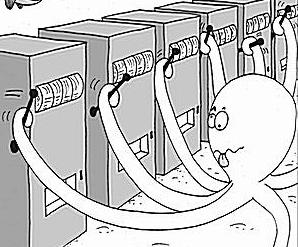
\includegraphics[height=4.5cm]{MABpieuvre}
    \end{center}
    \begin{center}
        An \blue agent \black facing \red arms \black in a Multi-Armed Bandit.
    \end{center}

    \pause
    \begin{center}
        \Huge NO!
    \end{center}
\end{frameO}

\begin{frameO}[Sequential resource allocation]
    \textbf{Clinical trials}
    \begin{itemize}
        \item $K$ treatments for a given symptom (with unknown effect)

        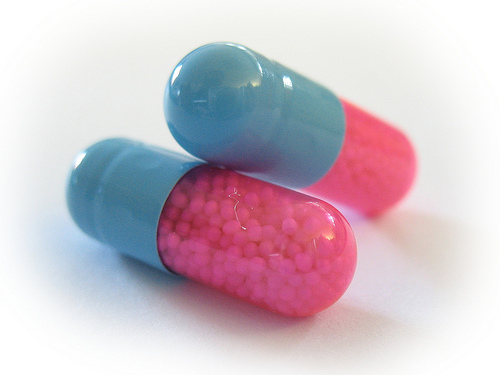
\includegraphics[width=0.12\linewidth]{medoc1.jpg}
        \hspace{0.05cm}
        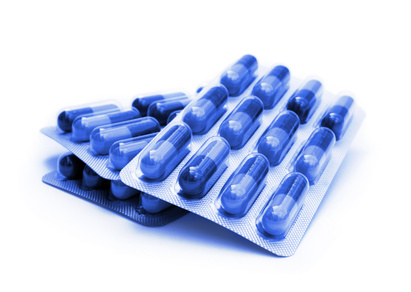
\includegraphics[width=0.12\linewidth]{medoc4.jpg}
        \hspace{0.05cm}
        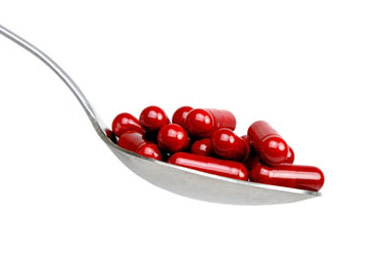
\includegraphics[width=0.12\linewidth]{medoc3.jpg}
        \hspace{0.05cm}
        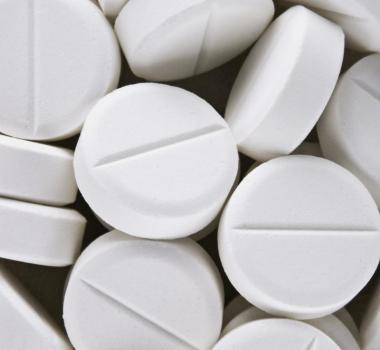
\includegraphics[width=0.12\linewidth]{medoc2.jpg}
        \hspace{0.05cm}
        
\includegraphics[width=0.12\linewidth]{medoc5.jpg}
        \hspace{0.05cm}
        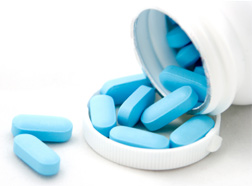
\includegraphics[width=0.12\linewidth]{medoc6.jpg}
        \hspace{0.05cm}

        \item What treatment should be allocated to the next patient based on responses observed on previous patients?
    \end{itemize}

    \vspace{0.2cm}

    \pause

    \textbf{Online advertisement}
    \begin{itemize}
        \item $K$ adds that can be displayed
        \vspace{0.1cm}

        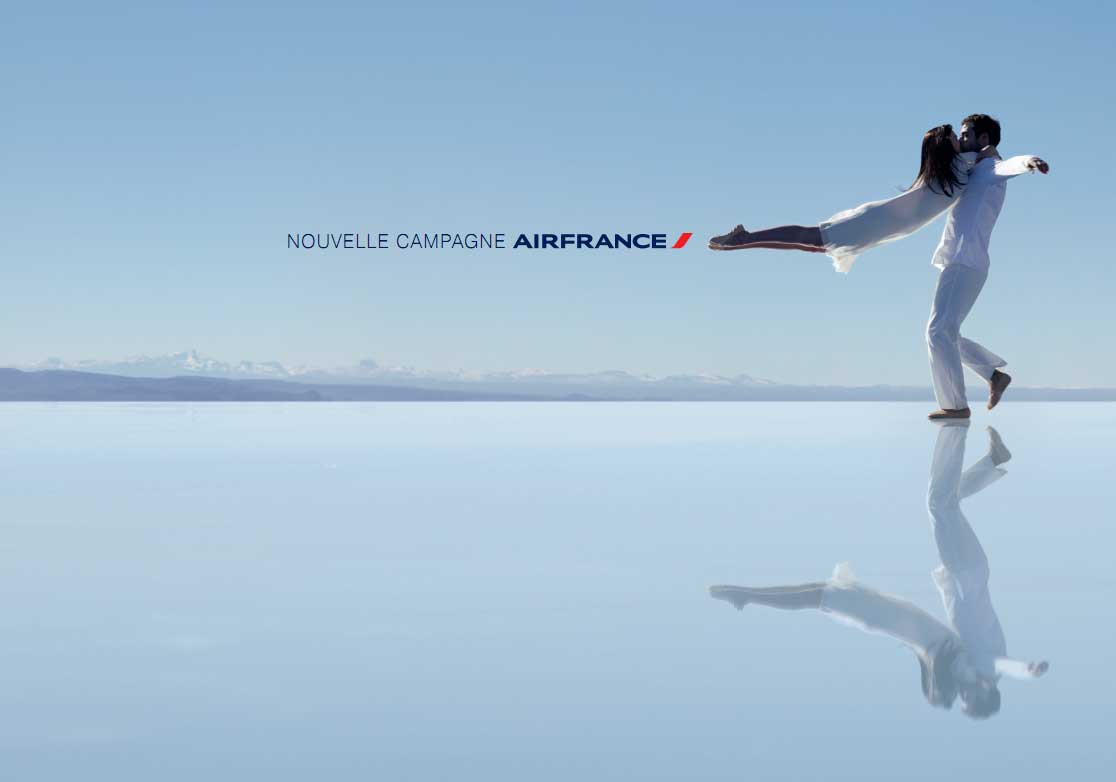
\includegraphics[height=0.15\paperheight]{ad6.jpg}
        \hspace{0.1cm}
        
\includegraphics[height=0.15\paperheight]{ad2.jpg}
        \hspace{0.1cm}
        
\includegraphics[height=0.15\paperheight]{ad4.jpg}
        \hspace{0.1cm}
        
\includegraphics[height=0.15\paperheight]{ad5.jpg}
        \hspace{0.05cm}

        \item Which add should be displayed for a user, based on the previous clicks of previous (similar) users?
    \end{itemize}

\end{frameO}

\begin{frameO}[Dynamic channel selection]

    \vspace{0.3cm}

    \textbf{Opportunistic Spectrum Access}
    \begin{itemize}
        \item $K$ radio channels (frequency bands)

              \hspace{0.4cm}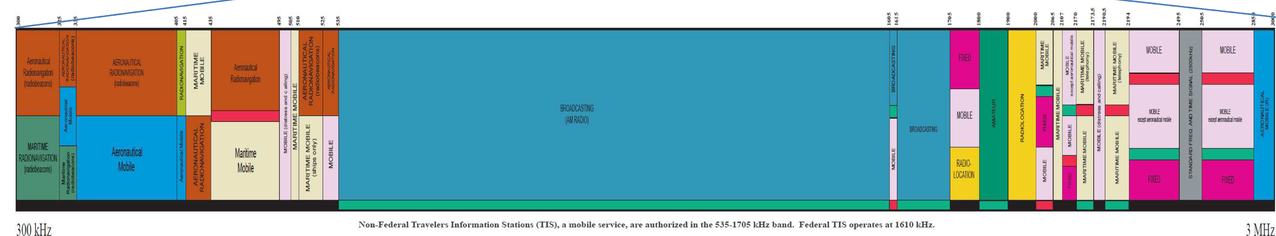
\includegraphics[height=0.17\paperheight]{spectrum}
        \item In which channel should a radio device send a packet based on the quality of its previous communications?
        \pause
        $\hookrightarrow$ \textcolor{blue}{see the next talk at 4pm !}
    \end{itemize}

    \vspace{0.1cm}

    \pause

    \textbf{Communications in presence of a central controller}
    \begin{itemize}
        \item $K$ assignments from users to antennas

              \hspace{2.5cm}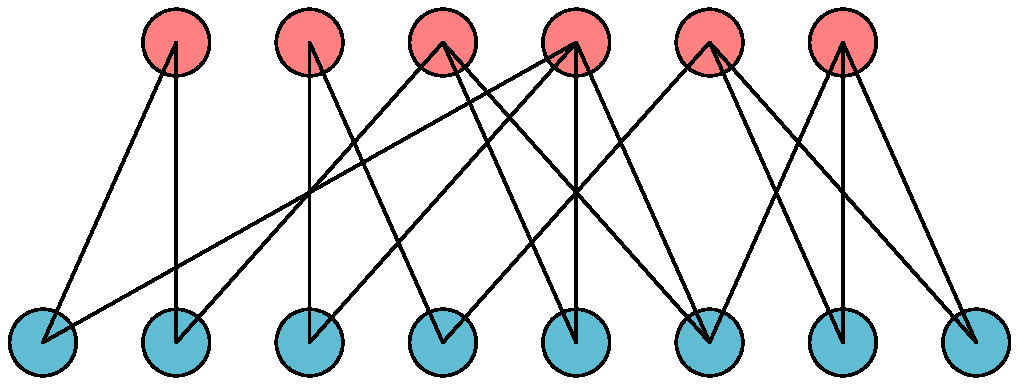
\includegraphics[height=0.2\paperheight]{assignements}
        \item How to select the next matching based on the throughput observed in previous communications?
    \end{itemize}

\end{frameO}



\begin{frameO}[Dynamic allocation of computational resources]

    \vspace{0.4cm}

    \textbf{Numerical experiments}:

    \vspace{-0.3cm}

    \begin{center}
        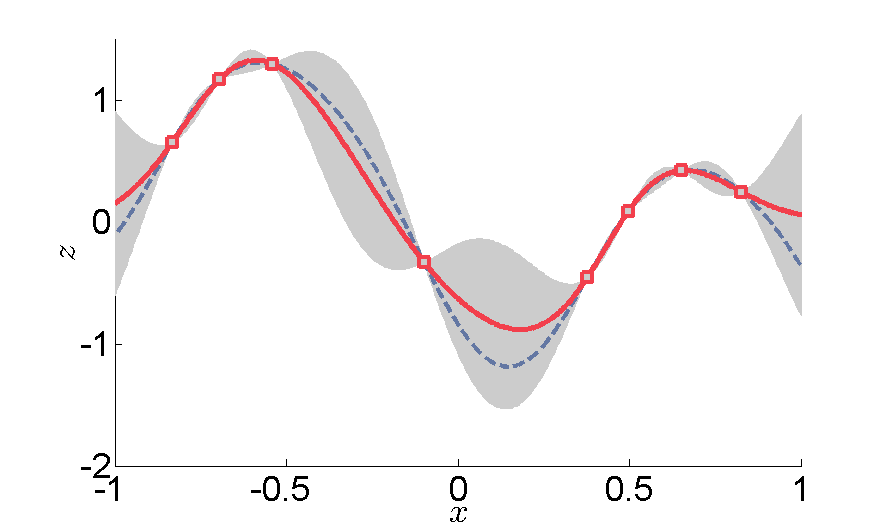
\includegraphics[height=2cm]{GP}
    \end{center}

    \vspace{-0.3cm}

    \begin{itemize}
        \item where to evaluate a costly function in order to find its maximum?
    \end{itemize}

    \pause

    \textbf{Artificial intelligence for games}:

    \begin{center}
        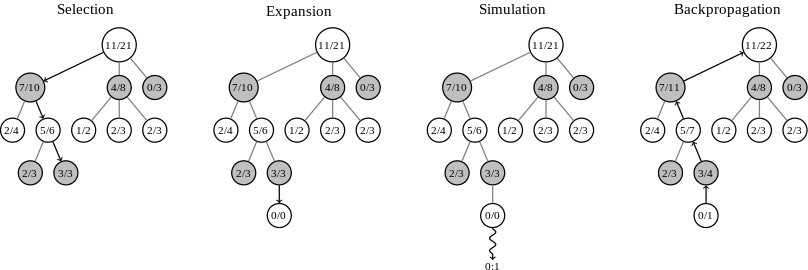
\includegraphics[height=2.2cm]{MCTSWiki}
    \end{center}

    \vspace{-0.5cm}

    \begin{itemize}
        \item where to choose the next evaluation to perform in order to find the best move to play next?
    \end{itemize}


\end{frameO}


\begin{frameO}[Why bandits now?]

    \begin{itemize}
        \item rewards maximization in a stochastic bandit model

              = \red the simplest Reinforcement Learning (RL) problem \black (one state)

        \item bandits showcase the important \red exploration/exploitation dilemma \black
        \item \red bandit tools \black are useful for RL

              (UCRL, bandit-based MCTS for planning in games...)

        \item a \red rich literature \black to tackle many specific applications

        \item bandits have application \red beyond RL \black(i.e. without ``reward'')
    \end{itemize}
\end{frameO}


\begin{frameO}[Outline of this talk]

    FIXME

\end{frameO}


%%% TITLE SLIDE FOR PART I


% standard slides for Part I

\setbeamertemplate{background canvas}{
\includegraphics[width=\paperwidth,height=\paperheight]{basrouge}}

\setbeamertemplate{footline}{\hspace{2cm} \raisebox{2.5ex}
    {\textcolor{white}{Lilian Besson \& Émilie Kaufmann - Intro to MAB}}\hfill
    \raisebox{2.5ex}
    {\textcolor{white}{23 September, 2019 - \insertframenumber \hspace{5mm} \null }}}

\section{Multi-armed Bandit}

\begin{frameO}[\alt<2>{The \blue Stochastic \color{white} Multi-Armed Bandit Setup}{The Multi-Armed Bandit Setup}]

    \alt<2>{\vspace{0.4cm}}{}

    \begin{center}
        $K$ \textbf{arms} $\leftrightarrow$ $K$ \alt<2>{\blue probability distributions \black : $\nu_a$ has mean $\blue\mu_a$}{rewards streams $(X_{a,t})_{t\in\N}$}
    \end{center}

    \begin{center}
        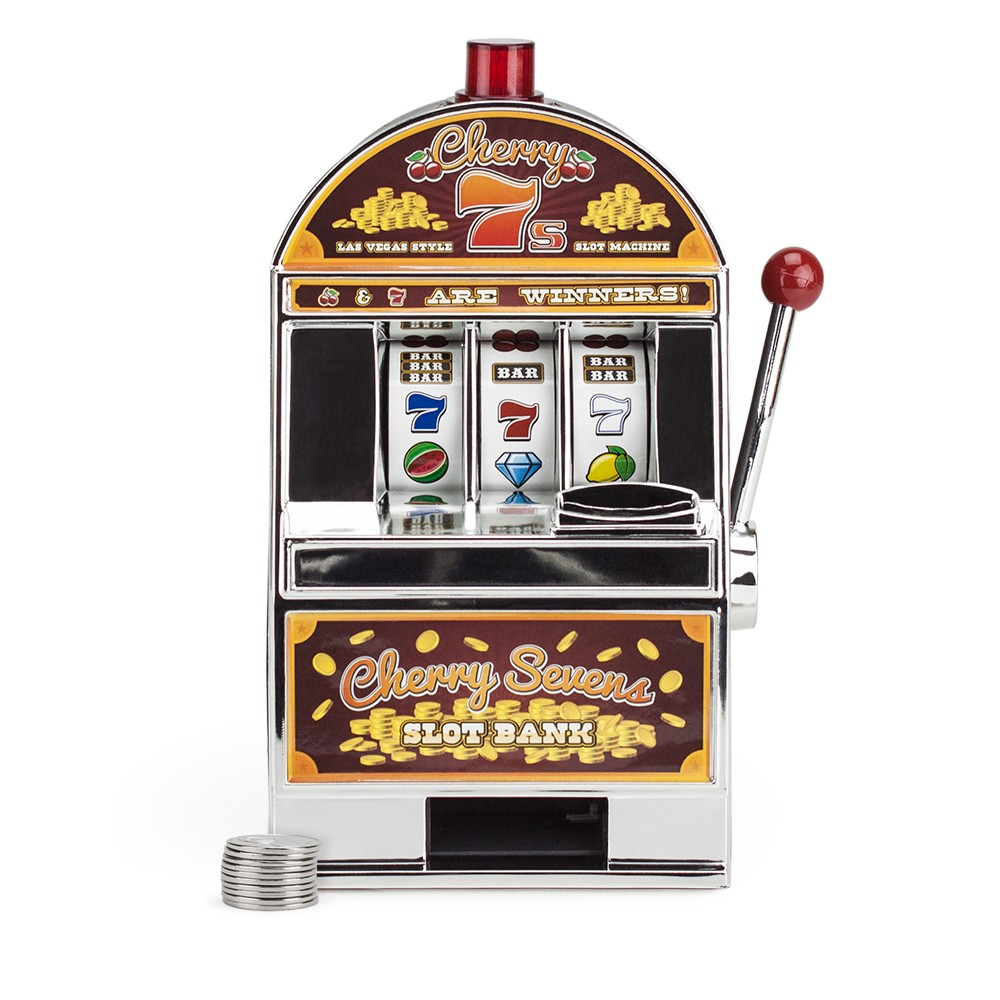
\includegraphics[height=0.15\textheight]{slot1.jpg}
        \hspace{0.4cm}
        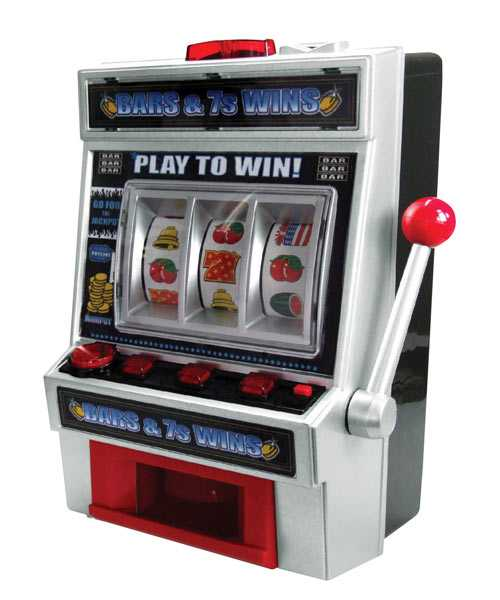
\includegraphics[height=0.15\textheight]{slot2.jpg}
        \hspace{0.4cm}
        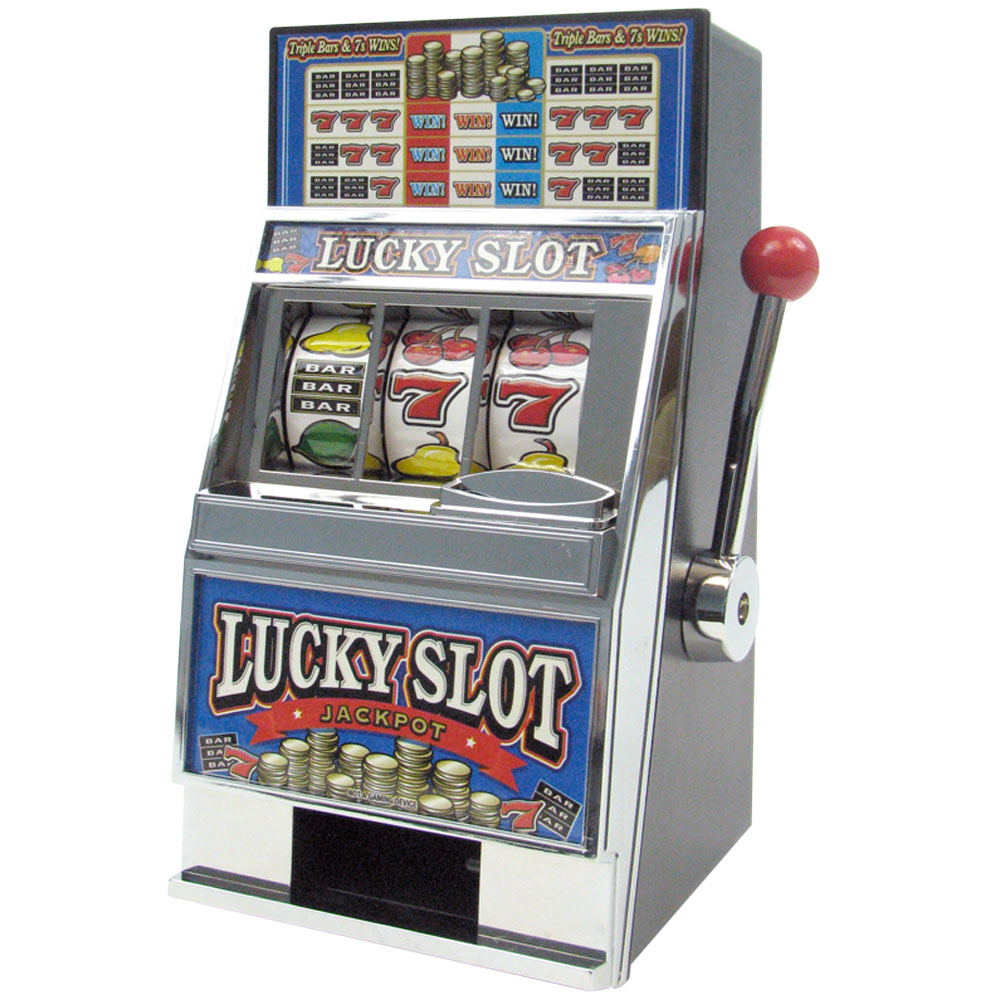
\includegraphics[height=0.15\textheight]{slot3.jpg}
        \hspace{0.4cm}
        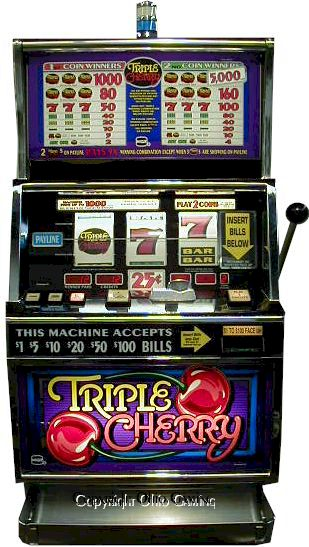
\includegraphics[height=0.15\textheight]{slot4.jpg}
        \hspace{0.5cm}
        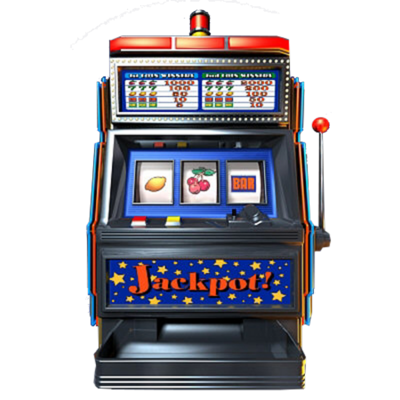
\includegraphics[height=0.15\textheight]{slot5.jpg}
        \hspace{0.4cm}
    \end{center}

    \vspace{-0.8cm}

    \[ \alt<2>{\blue\nu_1}{} \hspace{1.4cm} \alt<2>{\blue\nu_2}{} \hspace{1.4cm} \alt<2>{\blue\nu_3}{} \hspace{1.4cm} \alt<2>{\blue\nu_4}{} \hspace{1.4cm} \alt<2>{\blue\nu_5}{}\]

    \alt<2>{\vspace{-0.4cm}}{}

    At round $t$, an agent:
    \begin{itemize}
        \item chooses an  arm $A_t$
        \item receives a reward \alt<2>{$R_t = X_{A_t,t}\blue \sim \nu_{A_t}$}{$R_t = X_{A_t,t}$}
    \end{itemize}

    \vspace{0.2cm}

    \red Sequential \black sampling strategy (\textbf{bandit algorithm}):
    \[\red A_{t+1} = F_t (A_1,R_1,\dots,A_{t},R_{t})\black.\]
    \textbf{Goal:} Maximize \alt<2>{$\blue \bE\black\left[\sum_{t=1}^T R_t\right]$}{$\sum_{t=1}^T R_t$}.


\end{frameO}

\begin{frameO}[Discover bandits by playing this online demo!]

  \begin{center}
    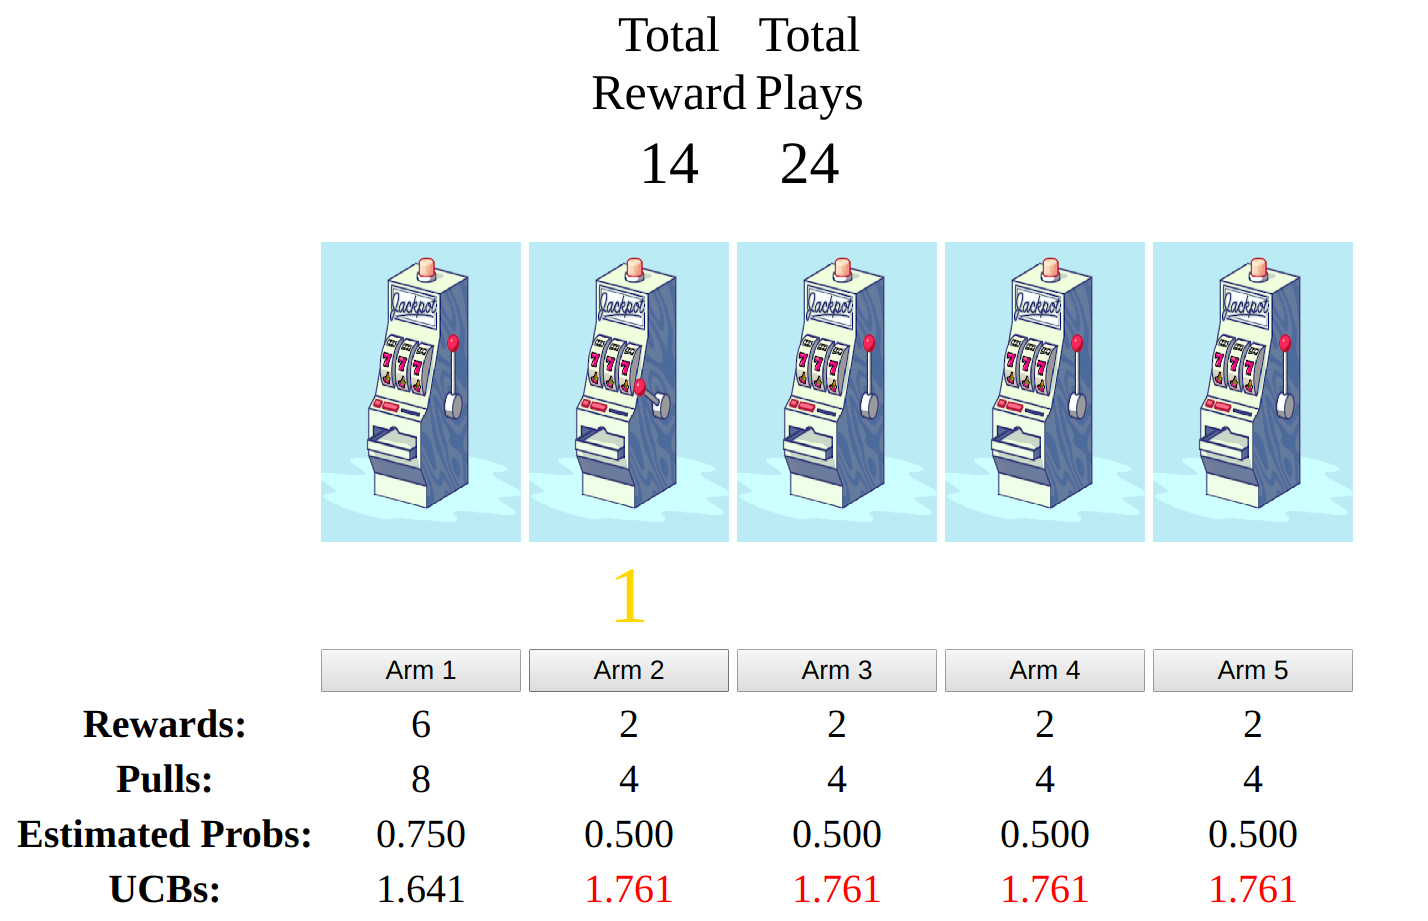
\includegraphics[width=0.75\textwidth]{example_of_a_5_arm_bandit_problem.png}
  \end{center}

  % \begin{small}
  $\hookrightarrow$ Interactive demo
    \href{https://perso.crans.org/besson/phd/MAB_interactive_demo/}{\textcolor{blue}{\texttt{perso.crans.org/besson/phd/MAB\_interactive\_demo/}}}\\
    % Ref: [Bandits Algorithms, Lattimore \& Szepesv{\'a}ri, 2019],
    % on \href{https://tor-lattimore.com/downloads/book/book.pdf}{\textcolor{blue}{\texttt{tor-lattimore.com/downloads/book/book.pdf}}}
  % \end{small}

\end{frameO}

\begin{frameO}[Clinical trials]

    \textbf{Historical motivation} \color{gray}[Thompson 1933]\color{black}

    \begin{center}
        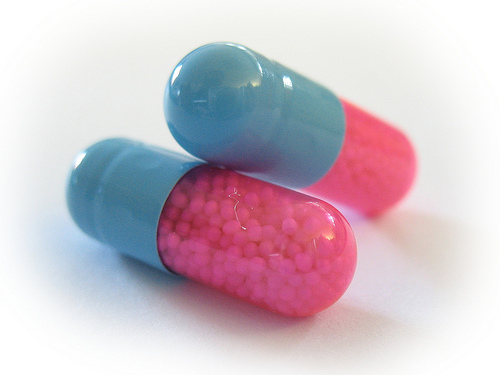
\includegraphics[width=0.12\linewidth]{medoc1.jpg}
        \hspace{0.3cm}
        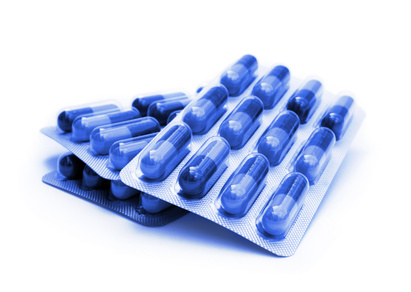
\includegraphics[width=0.12\linewidth]{medoc4.jpg}
        \hspace{0.3cm}
        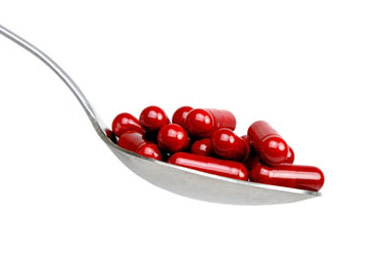
\includegraphics[width=0.12\linewidth]{medoc3.jpg}
        \hspace{0.5cm}
        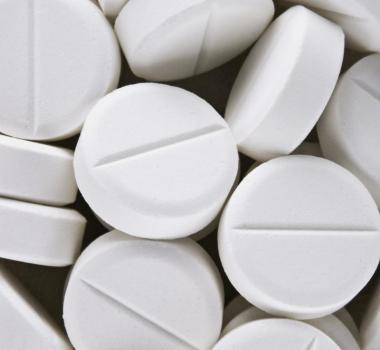
\includegraphics[width=0.12\linewidth]{medoc2.jpg}
        \hspace{0.5cm}
        
\includegraphics[width=0.12\linewidth]{medoc5.jpg}
        \hspace{0.3cm}
    \end{center}
    \vspace{-0.8cm}

    \hspace{-0.3cm}\[ \cB(\mu_1) \hspace{0.9cm} \cB(\mu_2) \hspace{0.9cm} \cB(\mu_3) \hspace{0.8cm} \cB(\mu_4) \hspace{0.9cm} \cB(\mu_5)\]

    For the $t$-th patient in a clinical study,

    \begin{itemize}
        \item chooses a \blue treatment $A_t$\black
        \item observes a \blue response $R_t \in \{0,1\} : \bP(R_t = 1 | A_t = a) = \mu_{a}$\black
    \end{itemize}

    \vspace{0.3cm}


    \textbf{Goal:} maximize the expected number of patients healed

\end{frameO}



\begin{frameO}[Online content optimization]

    \textbf{Modern motivation} ($\$\$\$\$$) \gray [Li et al, 2010] \black

    (recommender systems, online advertisement)


    \begin{center}
        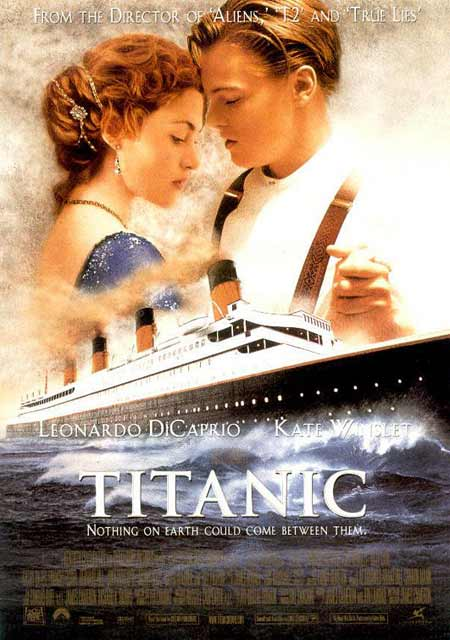
\includegraphics[height=0.15\textheight]{film1.jpg}
        \hspace{0.6cm}
        
\includegraphics[height=0.15\textheight]{film2.jpg}
        \hspace{0.6cm}
        
\includegraphics[height=0.15\textheight]{film3.jpg}
        \hspace{0.6cm}
        
\includegraphics[height=0.15\textheight]{film4.jpg}
        \hspace{0.6cm}
        
\includegraphics[height=0.15\textheight]{film5.jpg}
        \hspace{0.6cm}
    \end{center}

    \vspace{-0.8cm}

    \hspace{-0.2cm}\[ \nu_1 \hspace{1.4cm} \nu_2 \hspace{1.4cm} \nu_3 \hspace{1.4cm} \nu_4 \hspace{1.4cm} \nu_5\]

    For the $t$-th visitor of a website,
    \begin{itemize}
        \item recommend a  \blue movie $A_t$\black
        \item observe a \blue rating $R_t \sim \nu_{A_t}$\black \ (e.g. $R_t \in \{1,\dots,5\}$)
    \end{itemize}

    \vspace{0.3cm}

    \textbf{Goal:} maximize the sum of ratings


\end{frameO}

\begin{frameO}[Cognitive radios]

    \textbf{Opportunistic spectrum access} \gray [Anandkumar et al. 11]\black

    \begin{center}

        \emph{streams indicating channel quality}

        \vspace{0.3cm}

        \begin{tabular}{|c||c|c|c|c|c|c|c}
            \hline
            Channel $1$ & \cellcolor{blue!25}$X_{1,1}$ & $X_{1,2}$                    & \dots   & $X_{1,t}$                    & \dots   & $X_{1,T}$                    & $\sim \nu_1$ \\
            \hline
            Channel $2$ & $X_{2,1}$                    & \cellcolor{blue!25}$X_{2,2}$ & \dots   & $X_{2,t}$                    & \dots   & \cellcolor{blue!25}$X_{2,T}$ & $\sim \nu_2$ \\
            \hline
            $\dots$     & $\dots$                      & $\dots$                      & $\dots$ & $\dots$                      & $\dots$ & $\dots$                                     \\
            \hline
            Channel $K$ & $X_{K,1}$                    & $X_{K,2}$                    & \dots   & \cellcolor{blue!25}$X_{K,t}$ & \dots   & $X_{K,T}$                    & $\sim \nu_K$ \\
            \hline
        \end{tabular}
    \end{center}

    \vspace{0.2cm}

    At round $t$, the device:
    \begin{itemize}
        \item selects \blue{a channel} $A_t$\black
        \item observes the \blue quality of its communication  $R_t = X_{A_t,t} \in [0,1]$\black
    \end{itemize}

    \vspace{0.2cm}

    \textbf{Goal:} Maximize the overall quality of communications

\end{frameO}



\section{Performance measure and first strategies}


\begin{frameTI}
    \begin{center}
        \color{white} \Huge \textsc{Performance measure}

        \vspace{0.2cm}

        \huge \textsc{and first strategies}

    \end{center}
    \vspace*{-4pt}
\end{frameTI}

\begin{frameO}[Regret of a bandit algorithm]

    \bigskip

    \textbf{Bandit instance:} $\nu = (\nu_1,\nu_2, \dots,\nu_K)$, mean of arm $a$: $\mu_a = \bE_{X \sim \nu_a}[X]$.

    \[\red\mu_\star = \max_{a \in \{1,\dots,K\}} \mu_a \ \  \ \ \ a_\star = \argmax_{a \in \{1,\dots,K\}} \mu_a.\]
    \[\begin{array}{ccl}\text{Maximizing rewards} & \leftrightarrow & \text{selecting } a_\star \text{ as much as possible }         \\
                                           & \leftrightarrow & \text{minimizing the \blue regret } \gray \text{[Robbins, 52]}
        \end{array}\]

    \vspace{-0.4cm}

    \begin{eqnarray*}
        \blue \cR_\nu(\cA,T) \eqdef \black\underbrace{\blue T \mu_\star}_{\substack{\text{sum of rewards of}\\ \text{an oracle strategy} \\ \text{always selecting } a_\star}} \blue- \black\underbrace{\blue\bE\left[\sum_{t=1}^{T}R_{t}\right]}_{\substack{\text{sum of rewards of}\\\text{the strategy} \cA}}
    \end{eqnarray*}

    \vspace{-0.4cm}
    \pause

    \begin{orangeblock}{What regret rate can we achieve?}
        \begin{itemize}
            \item[\ding{220}] consistency: \black $\frac{\cR_\nu(\cA,T)}{T} \rightarrow 0$
            \item[\ding{220}] can we be more precise?
        \end{itemize}
    \end{orangeblock}
\end{frameO}

\begin{frameO}[Regret decomposition]

    \vspace{0.6cm}

    $N_a(t)$ : number of selections of arm $a$ in the first $t$ rounds

    $\Delta_a \eqdef \mu_\star -\mu_a$ : sub-optimality gap of arm $a$

    \begin{orangeblock}{Regret decomposition}
        \[\red\cR_\nu(\cA,T) = \sum_{a=1}^K \Delta_a \bE\left[N_a(T)\right].\]
    \end{orangeblock}

    \alt<2>{

        \vspace{0.6cm}

        A strategy with small regret should:
        \begin{itemize}
            \item select not too often arms for which $\Delta_a > 0$
            \item ... which requires to try all arms to estimate the values of the $\Delta_a$'s
        \end{itemize}

        \vspace{0.5cm}

        \red $\Rightarrow $ Exploration / Exploitation trade-off

    }
    {
        \textbf{Proof.}

        \vspace{-1cm}

        \begin{eqnarray*}
            \cR_\nu(\cA,T) & = & \mu_\star T - \bE \! \left[\sum_{t=1}^T X_{A_t,t}\right] = \mu_\star T - \bE \! \left[\sum_{t=1}^T \mu_{A_t} \right]\\
            & = & \bE\left[\sum_{t=1}^T (\mu_\star - \mu_{A_t})\right] \\
            &= & \sum_{a =1}^K \underbrace{(\mu_\star- \mu_a)}_{\Delta_a} \, \bE \biggl[ \underbrace{\sum_{t=1}^T\ind(A_t=a)}_{N_a(T)} \biggr]\,.
        \end{eqnarray*}}

\end{frameO}


\begin{frameO}[Two naive strategies]

    \vspace{0.4cm}

    \begin{itemize}
        \item \textbf{Idea 1 :} \begin{orangeblock}{}Draw each arm $T/K$ times\end{orangeblock}
    \end{itemize}
    \color{red}$\Rightarrow$ EXPLORATION \color{black}

    \vspace{-0.8cm}

    \[\cR_\nu(\cA,T) = \left(\frac{1}{K}\sum_{a : \mu_a > \mu_\star} \Delta_a\right) T = \alert{\Omega(T)} \]

    \pause

    \begin{itemize}
        \item \textbf{Idea 2 :} Always trust the empirical best arm
    \end{itemize}
    \begin{orangeblock}{}
        \[A_{t+1}=\underset{a \in \{1,\dots,K\}}{\text{argmax}} \ \blue \hat{\mu}_a(t)\]
        \vspace{-0.5cm}

        where

        \vspace{-0.6cm}

        \[\blue \hat{\mu}_a(t) =\frac{1}{N_a(t)}\sum_{s=1}^t X_{a,s} \ind_{(A_s=a)}\]

        \vspace{-0.3cm}

        is an estimate of the unknown mean $\mu_a$.


    \end{orangeblock}

    \color{red}$\Rightarrow$ EXPLOITATION \color{black}

    \vspace{-0.8cm}

    \[\hspace{1.5cm}\cR_\nu(\cA,T) \geq  (1-\mu_1)\times \mu_2 \times (\mu_1 - \mu_2) T  = \alert{\Omega(T)} \]
    \begin{center}\vspace{-0.2cm}
        \hspace{1.5cm}(Bernoulli arms)
    \end{center}


\end{frameO}


\begin{frameO}[A better idea: Explore-Then-Commit]

    \alt<3>{\vspace{0.3cm}}{}

    \begin{orangeblock}{}
        Given $ m \in \{ 1, \dots, T/K\}$,
        \begin{itemize}
            \item draw each arm $m$ times
            \item compute the empirical best arm $\hat{a} = \text{argmax}_{a} \ \hat{\mu}_a(Km)$
            \item keep playing this arm until round $T$

                  \vspace{-0.4cm}

                  \[A_{t+1} = \hat{a} \ \ \text{for} \ t \geq Km\]
        \end{itemize}
        \color{red}$\Rightarrow$ EXPLORATION followed by EXPLOITATION\color{black}
    \end{orangeblock}
    \pause

    \vspace{0.2cm}


    \underline{Analysis for two arms}. $\mu_1 > \mu_2$,  $\textcolor{blue}{\Delta := \mu_1 - \mu_2}$.

    \vspace{-0.5cm}

    \begin{eqnarray*}\mathcal{R}_\nu(\texttt{ETC},T) & = & \Delta \bE[N_2(T)] \\
        & = & \Delta \bE\left[ m + (T - Km)\ind\left(\hat{a} = 2\right)\right] \\
        & \leq &\Delta m + (\Delta T) \times \alt<3>{\red \bP\left(\hat{\mu}_{2,m} \geq \hat{\mu}_{1,m}\right)}{\bP\left(\hat{\mu}_{2,m} \geq \hat{\mu}_{1,m}\right)}
    \end{eqnarray*}

    \vspace{-0.3cm}

    $\hat{\mu}_{a,m}$: empirical mean of the first $m$ observations from arm
    $a$

    \alt<3>{\red $\rightarrow$ requires a concentration inequality}{}
\end{frameO}


\begin{frameO}[A better idea: Explore-Then-Commit]

    \vspace{0.3cm}
    \begin{orangeblock}{}
        Given $ m \in \{ 1, \dots, T/K\}$,
        \begin{itemize}
            \item draw each arm $m$ times
            \item compute the empirical best arm $\hat{a} = \text{argmax}_{a} \ \hat{\mu}_a(Km)$
            \item keep playing this arm until round $T$

                  \vspace{-0.4cm}

                  \[A_{t+1} = \hat{a} \ \ \text{for} \ t \geq Km\]
        \end{itemize}
        \color{red}$\Rightarrow$ EXPLORATION followed by EXPLOITATION\color{black}
    \end{orangeblock}
    \vspace{0.2cm}


    \underline{Analysis for two arms}. $\mu_1 > \mu_2$,  $\textcolor{blue}{\Delta := \mu_1 - \mu_2}$.

    \textbf{Assumption 1:} $\nu_1,\nu_2$ are \red bounded in $[0,1]$\black.

    \vspace{-0.7cm}

    \begin{eqnarray*}\mathcal{R}_\nu(T) & = & \Delta \bE[N_2(T)] \\
        & = & \Delta \bE\left[ m + (T - Km)\ind\left(\hat{a} = 2\right)\right] \\
        & \leq &\Delta {m} + (\Delta T) \times \exp(- {m\Delta^2}/{2})
    \end{eqnarray*}

    \vspace{-0.3cm}

    $\hat{\mu}_{a,m}$: empirical mean of the first $m$ observations from arm
    $a$

    $\rightarrow$ \red Hoeffding's inequality
\end{frameO}



\begin{frameO}[A better idea: Explore-Then-Commit]

    \vspace{0.3cm}
    \begin{orangeblock}{}
        Given $ m \in \{ 1, \dots, T/K\}$,
        \begin{itemize}
            \item draw each arm $m$ times
            \item compute the empirical best arm $\hat{a} = \text{argmax}_{a} \ \hat{\mu}_a(Km)$
            \item keep playing this arm until round $T$

                  \vspace{-0.4cm}

                  \[A_{t+1} = \hat{a} \ \ \text{for} \ t \geq Km\]
        \end{itemize}
        \color{red}$\Rightarrow$ EXPLORATION followed by EXPLOITATION\color{black}
    \end{orangeblock}
    \vspace{0.2cm}


    \underline{Analysis for two arms}. $\mu_1 > \mu_2$,  $\textcolor{blue}{\Delta := \mu_1 - \mu_2}$.

    \textbf{Assumption 2:} $\nu_1 =\cN(\mu_1,\sigma^2),\nu_2 = \cN(\mu_2,\sigma^2)$ are \red Gaussian arms\black.

    \vspace{-0.7cm}

    \begin{eqnarray*}\mathcal{R}_\nu(\texttt{ETC},T) & = & \Delta \bE[N_2(T)] \\
        & = & \Delta \bE\left[ m + (T - Km)\ind\left(\hat{a} = 2\right)\right] \\
        & \leq &\Delta \alt<2>{\blue m\black}{m} + (\Delta T) \times \exp(- {\alt<2>{\blue m \black}{m}\Delta^2}/{4\sigma^2})
    \end{eqnarray*}

    \vspace{-0.3cm}

    $\hat{\mu}_{a,m}$: empirical mean of the first $m$ observations from arm
    $a$

    $\rightarrow$ \red Gaussian tail inequality
\end{frameO}


\begin{frameO}[A better idea: Explore-Then-Commit]

    \vspace{0.3cm}
    \begin{orangeblock}{}
        Given $ m \in \{ 1, \dots, T/K\}$,
        \begin{itemize}
            \item draw each arm $m$ times
            \item compute the empirical best arm $\hat{a} = \text{argmax}_{a} \ \hat{\mu}_a(Km)$
            \item keep playing this arm until round $T$

                  \vspace{-0.4cm}

                  \[A_{t+1} = \hat{a} \ \ \text{for} \ t \geq Km\]
        \end{itemize}
        \color{red}$\Rightarrow$ EXPLORATION followed by EXPLOITATION\color{black}
    \end{orangeblock}
    \vspace{0.2cm}


    \underline{Analysis for two arms}. $\mu_1 > \mu_2$,  $\textcolor{blue}{\Delta := \mu_1 - \mu_2}$.

    \textbf{Assumption:}
    $\nu_1 =\cN(\mu_1,\sigma^2),\nu_2 = \cN(\mu_2,\sigma^2)$ are \red Gaussian arms\black.

    For $\blue m = \frac{4\sigma^2}{\Delta^2}\ln\left(\frac{T\Delta^2}{4\sigma^2}\right)$,

    \vspace{-0.3cm}

    \[\cR_\nu(\texttt{ETC},T) \leq \frac{4\sigma^2}{\Delta}\left[\ln\left(\frac{T\Delta^2}{2}\right) + 1\right].\]

    \vspace{-0.4cm}

    \pause

    \begin{itemize}
        \item[$\bm +$] logarithmic regret!
        \item[$\bm -$] requires the knowledge of $T$ \red and $\Delta$
    \end{itemize}


\end{frameO}





\begin{frameO}[Sequential Explore-Then-Commit (2 Gaussian arms)]

    \vspace{0.3cm}

    \begin{itemize}
        \item  explore uniformly until the \blue random time \black
    \end{itemize}
    \vspace{-0.3cm}

    \[\hspace{-1cm}\blue \tau = \inf \left\{t \in \N : |\hat{\mu}_1(t) - \hat{\mu}_2(t) | > \sqrt{\frac{8\sigma^2\ln(T/t)}{t}}\right\}  \]



    \vspace{-0.9cm}

    \begin{center}
        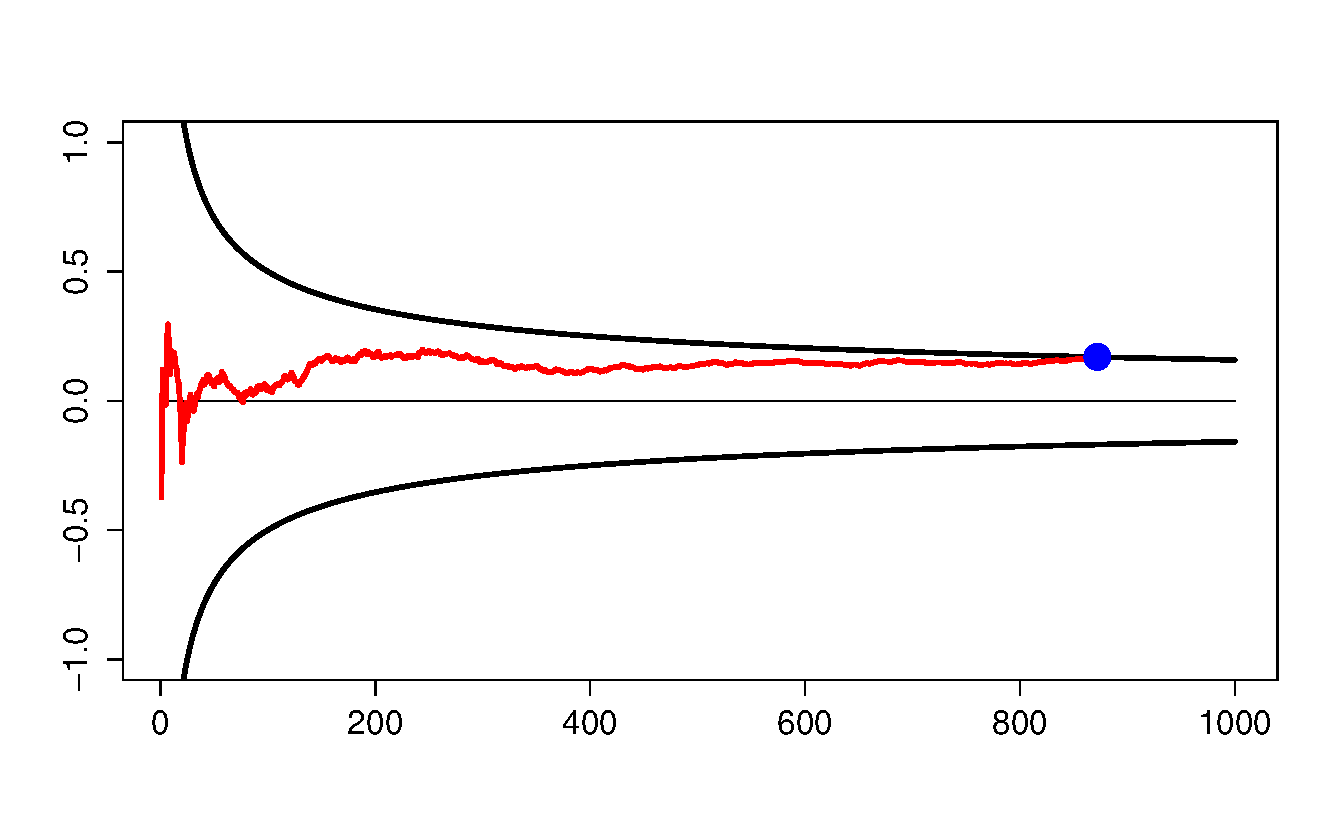
\includegraphics[width=0.5\linewidth]{figGaussianElimination}
    \end{center}


    \vspace{-0.6cm}


    \begin{itemize}
        \item $\blue \hat{a}_\tau = \argmax{}_{a} \ \hat{\mu}_a(\tau)$ and $(A_{t+1} = \hat{a}_\tau)$ for $t \in \{\tau+1, \dots, T\}$
    \end{itemize}

    \vspace{-0.2cm}

    \[
        \cR_\nu(\texttt{S-ETC},T)  \leq  \red \frac{4\sigma^2}{\Delta}\ln\left(T\Delta^2\right)\black \ + C \sqrt{\ln(T)}.\]

    \vspace{-0.3cm}

    \begin{itemize}
        \item[\ding{220}] same regret rate, without knowing $\Delta$ \gray [Garivier et al. 2016]
    \end{itemize}


\end{frameO}

\begin{frameO}[Numerical illustration]

    \[\nu_1 = \cN(1,1) \ \ \nu_2 = \cN(1.5,1)\]

    \begin{minipage}{0.49\linewidth}
        \centering
        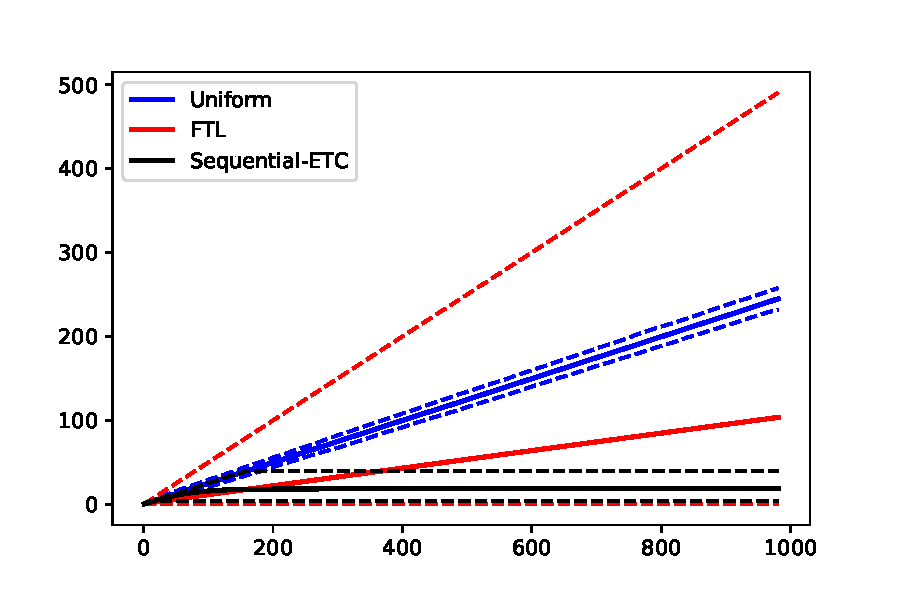
\includegraphics[width=\textwidth]{3algos}
    \end{minipage}
    \begin{minipage}{0.49\linewidth}
        \centering
        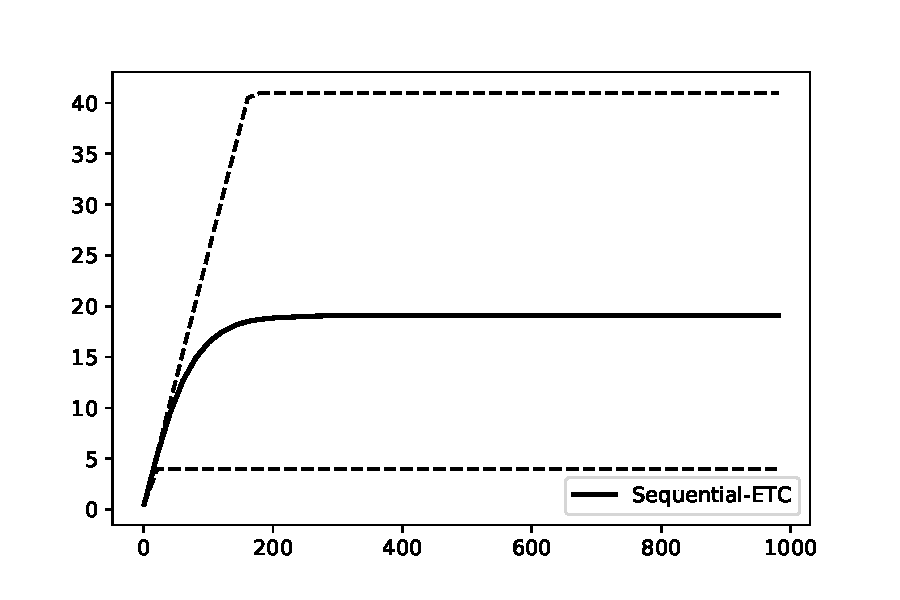
\includegraphics[width=\textwidth]{1algos}
    \end{minipage}
    \begin{center}
        Expected regret estimated over $N=500$ runs for Sequential-ETC versus our two naive baselines.

        {\small (dashed lines: empirical 0.05\% and 0.95\% quantiles of the regret) }
    \end{center}



\end{frameO}


\begin{frameO}[Is this a good regret rate?]

    \vspace{0.3cm}

    For two-armed Gaussian bandits,
    \[
        \cR_\nu(\texttt{ETC},T)  \lesssim  \red \frac{4\sigma^2}{\Delta}\ln\left(T\Delta^2\right)\black.\]

    \vspace{-0.3cm}

    \begin{itemize}
        \item[\ding{220}] problem-dependent logarithmic regret bound
    \end{itemize}

    \textbf{Observation:} blows up when $\Delta$ tends to zero...
    \begin{eqnarray*}
        \cR_\nu(\texttt{ETC},T)  &\lesssim& \min \left[\frac{4\sigma^2}{\Delta}\ln\left(T\Delta^2\right) , \blue\Delta T\black\right] \\
        & \leq & \sqrt{T} \min_{u > 0} \left[\frac{4\sigma^2}{u}\ln(u^2) ; u\right] \\
        & \leq & \red C \sqrt{T}\black.
    \end{eqnarray*}

    \vspace{-0.3cm}

    \begin{itemize}
        \item[\ding{220}] problem-independent square-root regret bound
    \end{itemize}


\end{frameO}

\begin{frameTI}
    \begin{center}
        {\textcolor{white} {\Huge \textsc{Best possible regret?} }}

        \vspace{0.5cm}

        {\textcolor{white} {\huge \textsc{Lower Bounds} }}
    \end{center}
    \vspace*{-4pt}
\end{frameTI}


\begin{frameO}[The Lai and Robbins lower bound]

    \vspace{0.3cm}

    \textbf{Context:} a \blue parametric bandit model \black where each arm is parameterized by its mean $\nu =(\nu_{\mu_1},\dots,\nu_{\mu_K})$, $\mu_a \in \cI$.
    \[\nu \ \ \leftrightarrow \ \ \bm\mu = (\mu_1,\dots,\mu_K)\]


    \textbf{Key tool:} \blue Kullback-Leibler divergence\black.

    \begin{orangeblock}{Kullback-Leibler divergence}

        \alt<3>{\vspace{-0.2cm}}{}

        \[
            \red \mathrm{kl}(\mu,\mu')  \black : =   \alt<3>{\mu\ln \left(\frac{\mu}{\mu'}\right) + (1-\mu) \ln \left(\frac{1-\mu}{1-\mu'}\right) \ \ \ (\text{Bernoulli bandits})}{\alt<2>{\frac{(\mu - \mu')^2}{2\sigma^2} \ \ \ (\text{Gaussian bandits})}{\text{KL}\left(\nu_\mu,\nu_{\mu'}\right) =\bE_{X \sim \nu_{\mu}}\left[\ln \frac{d\nu_{\mu}}{d\nu_{\mu'}}(X)\right]}}
        \]


        \vspace{-0.3cm}

    \end{orangeblock}
    \begin{orangeblock}{Theorem \color{gray} [Lai and Robbins, 1985]}
        For uniformly efficient algorithms ($\cR_{\bm\mu}(\cA,T)=\mathcal{o}(T^\alpha)$ for all $\alpha\in (0,1)$ and $\bm \mu \in \cI^K$),

        \vspace{-0.4cm}

        \[
            \color{red}\mu_a<\mu_\star \Rightarrow \liminf_{T\rightarrow\infty}\frac{\bE_{\bm \mu}[N_{a}(T)]}{\ln T}\geq \frac{1}{\kl(\mu_a,\mu_\star)}\color{black}
        \]

        \vspace{-0.3cm}

    \end{orangeblock}

\end{frameO}

\begin{frameO}[Some room for better algorithms?]

    \vspace{0.3cm}

    \begin{itemize}
        \item for two-armed Gaussian bandits, ETC satisfies
              \[
                  \cR_\nu(\mathrm{ETC},T)  \lesssim  \red \frac{4\sigma^2}{\Delta}\black \ln\left(T\Delta^2\right),\]
              with $\Delta = |\mu_1 - \mu_2|$.
    \end{itemize}

    \begin{itemize}
        \item the Lai and Robbins' lower bound yields, for large values of $T$,
              \[
                  \cR_\nu(\cA,T)  \gtrsim  \red \frac{2\sigma^2}{\Delta}\black \ln\left(T\Delta^2\right),\]
              as $\kl(\mu_1,\mu_2) = \frac{(\mu_1 - \mu_2)^2}{2 \sigma^2}$.
    \end{itemize}

    \begin{itemize}
        \item[\ding{220}] Explore-Then-Commit is not \blue asymptotically optimal \black.
    \end{itemize}


\end{frameO}


\begin{frameO}[Behind the lower bound: a change of distribution]

    \vspace{0.3cm}

    Lower bounds rely on \red changes of distributions\black.

    \vspace{0.2cm}

    Fix $\cE \in \cF_t = \sigma(A_1,R_1,\dots,A_t,R_t)$.
    \begin{align}
        \bP_{\red\bm\lambda\black}(\blue \cE\black) & =  \int \ind_\cE(r_1,\dots,r_t) \,d\bP_{\bm\lambda}^{R_1,\dots,R_t}(r_1,\dots,r_t)\nonumber                                                                                                    \\
                                                    & =  \int \ind_\cE(r_1,\dots,r_t) \frac{d\bP_{\bm\lambda}^{R_1,\dots,R_t}(r_1,\dots,r_t)}{d\bP_{\bm\mu}^{R_1,\dots,R_t}(r_1,\dots,r_t)} \,d\bP_{\bm\mu}^{R_1,\dots,R_t}(r_1,\dots,r_t) \nonumber \\
        % &=  \int \ind_C(x_1,\dots,x_t) \frac{\ell(X_1,\dots,X_t ; \lambda)}{\ell(X_1,\dots,X_t ; \mu)} \,d\bP_{\mu}^{X_1,\dots,X_t}(x_1,\dots,x_t)\nonumber \\
                                                    & =  \bE_{\red \bm\mu\black}\Big[\blue\ind_{\cE}\black \exp\big(-L_t(\bm\mu,\bm\lambda)\big)\Big]\nonumber,
    \end{align}
    where $L_t(\bm\mu,\bm\lambda)$ denotes the log-likelihood ratio of the observations:
    \[L_t(\bm\mu,\bm\lambda) := \ln \frac{\ell(R_1,\dots,R_t ; \bm\mu)}{\ell(R_1,\dots,R_t ; \bm\lambda)}.\]

    \begin{itemize}
        \item \textbf{Idea}: relate the probability of the same event ($\blue \cE$) under two different bandit models ($\red \bm \lambda$ and $\red \bm \mu$).
    \end{itemize}


\end{frameO}


\begin{frameO}[Behind the lower bound: a change of distribution]

    \vspace{0.3cm}

    \begin{itemize}
        \item a sophisticated form of change of distribution
    \end{itemize}

    \begin{alertblock}{Lemma \color{gray}[K., Cappé, Garivier 16]}
        Let $\bm \mu$ and $\bm \lambda$ be two bandit models. For all event $\cE \in \cF_{T}$,

        \vspace{-0.4cm}

        \[\sum_{a=1}^K \bE_{\bm \mu}[N_a(T)]\times \kl(\mu_a,\lambda_a) \geq \mathrm{kl}_{\text{Ber}}(\bP_{\bm \mu}(\cE),\bP_{\bm \lambda}(\cE)).\]
    \end{alertblock}

    \pause

    \textbf{Proof.} 1. Under a parametric bandit model, one can prove that

    \vspace{-0.4cm}

    \[\bE_{\bm \mu}[L_T(\bm \mu,\bm \lambda)] = \sum_{a=1}^K \bE_{\bm \mu}[N_a(T)]\times \kl(\mu_a,\lambda_a).\]


    2. An information-theoretic argument:

    \vspace{-0.5cm}

    \begin{eqnarray*}
        \bE_{\bm \mu}[L_T(\bm \mu,\bm \lambda)] & = & \mathrm{KL}\left(\bP_{\bm\mu}^{R_1,\dots,R_T},\bP_{\bm\lambda}^{R_1,\dots,R_T}\right) \\
        &\geq & \mathrm{kl}_{\text{Ber}}(\bP_{\bm\mu}(\cE),\bP_{\bm \lambda}(\cE)) \ \ \text{for any } \cE \in \cF_{T}
    \end{eqnarray*}

    \vspace{-0.2cm}

    \color{gray} \hspace{1.5cm}[Garivier et al. 16]\color{black}



\end{frameO}


\begin{frameO}[Behind the lower bound: a change of distribution]

    \vspace{0.3cm}

    \begin{itemize}
        \item How to use it?
    \end{itemize}

    \vspace{-0.2cm}


    \begin{alertblock}{Lemma \color{gray}[K., Cappé, Garivier 16]}
        Let $\bm \mu$ and $\bm \lambda$ be two bandit models. For all event $\cE \in \cF_{T}$,

        \vspace{-0.4cm}

        \[\sum_{a=1}^K \bE_{\bm \mu}[N_a(T)]\times \kl(\mu_a,\lambda_a) \geq \mathrm{kl}_{\text{Ber}}(\bP_{\bm \mu}(\cE),\bP_{\bm \lambda}(\cE)).\]
    \end{alertblock}


    \vspace{-0.3cm}

    \begin{center}
        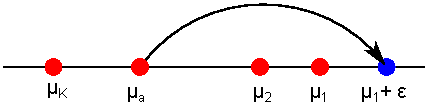
\includegraphics[height=1cm]{changement}
    \end{center}

    \vspace{-0.5cm}

    arm 1 is optimal under $\bm \mu$

    arm $a$ is optimal under $\bm \lambda =(\mu_1,\dots,\mu_{a-1},\blue\mu_1 + \varepsilon\black,\mu_{a+1},\dots,\mu_K)$

    \pause
    \alt<3>{\[\red \bE_{\bm\mu}[N_a(T)] \gtrsim \frac{\ln(T)}{\kl(\mu_a,\mu_\star + \varepsilon)}\]\vspace{-0.4cm}\begin{center}for large values of $T$                                                                                                                                                                                        \end{center}
    }{
    \begin{itemize}
        \item[\ding{220}]
              $\sum_{a=1}^K \bE_{\bm \mu}[N_a(T)]\times \kl(\mu_a,\lambda_a) = \red\bE_{\bm \mu}[N_a(T)] \kl(\mu_a,\mu_1+\varepsilon)$ \\
        \item[\ding{220}] Picking  $\blue \cE_T = (N_1(T) > T/2)\black$,
    \end{itemize}
    \[\red \mathrm{kl}_{\text{Ber}}(\bP_{\bm \mu}(\cE_T),\bP_{\bm \lambda}(\cE_T))\sim \ln(T)\]
    % \small as $\bP_{\bm \mu}(\cE_T) \sim 1$ and $\bP_{\bm \lambda}(\cE_T) \leq o(T^\alpha)/T$ (uniform efficiency).
    }

\end{frameO}

\begin{frameO}[The Lai and Robbins lower bound]

    \vspace{0.2cm}

    \textbf{Context:} a simple \blue parametric bandit model \black $\nu =(\nu_{\mu_1},\dots,\nu_{\mu_K})$, $\mu_a \in \cI$.

    \begin{orangeblock}{Lai and Robbins' lower bound \gray[1985]}
        For uniformly efficient algorithm,

        \vspace{-0.2cm}

        \[
            \color{red}\mu_a<\mu_\star \Rightarrow \liminf_{T\rightarrow\infty}\frac{\bE_{\bm \mu}[N_{a}(T)]}{\ln T}\geq \frac{1}{\kl(\mu_a,\mu_\star)}\color{black}
        \]

        \vspace{-0.3cm}

    \end{orangeblock}

    \begin{itemize}
        \item[\ding{220}] can be extended to cover \blue more general classes of bandit instances \black
    \end{itemize}

    \begin{orangeblock}{Burnetas and Katehakis' lower bound \gray[1996]}

        For any bandit such that $\nu_a\in\cD_a$.
        For any {uniformly efficient} strategy knowing $\cD_1,\dots,\cD_K$,

        \vspace{-4mm}
        \[\red
            \forall a: \mu_a<\mu_\star\quad
            \liminf_{T\to\infty}\frac{\bE[N_{a}(T)]}{\ln T} \geq \frac{1}{\cK_{a}(\nu_a,\mu_\star)},\]
        where $\cK_{a}(\nu_a,\mu_\star)= \inf \{\KL(\nu_a,\nu) : \nu\in\cD_a,\bE_{X \sim \nu}[X]>\mu_\star\}.$

    \end{orangeblock}


\end{frameO}


\begin{frameO}[A distribution-independent lower bound]

    \begin{orangeblock}{Theorem \gray[Cesa-Bianchi and Lugosi, 06][Bubeck and Cesa-Bianchi, 12]}
        Fix $T\in \N$. For every bandit algorithm $\cA$, there exists a stochastic bandit model $\nu$ with rewards supported in $[0,1]$ such that
        \[\cR_\nu(\cA,T) \geq \frac{1}{20}\red \sqrt{KT}\black\]
    \end{orangeblock}

    \begin{itemize}
        \item worse-case model:
              \[\left\{\begin{array}{ccl}
                      \nu_a & = & \cB(1/2) \ \ \text{for all} \ \ a\neq i \\
                      \nu_i & = & \cB(1/2+\varepsilon)
                  \end{array}\right.\]

              with $\varepsilon \simeq \sqrt{K/T}$.
    \end{itemize}


\end{frameO}


%
% \begin{frameO}[Some driving questions in the bandit literature]
%
% Since the work of Lai and Robbins, some focus has been put on finding algorithms...
%
% \vspace{0.3cm}
%
% \begin{itemize}
%  \item whose regret is asymptotically \red matching the existing lower bound\black, at least in simple parametric bandit
%  \item with \red finite-time \black upper bound on their regret
%  \item that are \red efficient \black in practice and easy to implement
%  \item that are \red easy to generalize \black to more \blue complex, structured\black, bandits
%  \item that are simultaneously optimal in a \red distribution-dependent and worst-case sense \black
% \end{itemize}
%
% \hfill $\dots$
%
% \end{frameO}


\begin{frameTI}
    \begin{center}
        \textcolor{white}{\Huge \textsc{Mixing Exploration and}}

        \vspace{0.2cm}

        \textcolor{white}{\Huge\textsc{Exploitation}}
        %\vspace{0.5cm}

        %{\textcolor{white} {\huge \textsc{Lower Bounds} }}
    \end{center}
    \vspace*{-4pt}
\end{frameTI}

\begin{frameO}[A simple strategy: $\varepsilon$\texttt{-greedy}]

    The $\varepsilon$\texttt{-greedy} rule \color{gray} [Sutton and Barton, 98] \black is the simplest way to alternate exploration and exploitation.

    \begin{orangeblock}{$\varepsilon$\texttt{-greedy} strategy}
        At round $t$,
        \begin{itemize}
            \item with probability $\varepsilon$
                  \[A_t \sim \cU(\{1,\dots,K\})\]
            \item with probability $1-\varepsilon$
                  \[A_t = \argmax_{a = 1,\dots,K} \ \hat{\mu}_a(t).\]
        \end{itemize}
    \end{orangeblock}

    \begin{itemize}
        \item[\ding{220}] \underline{Linear regret}: $\cR_\nu\left(\varepsilon\texttt{-greedy},T\right) \geq \varepsilon\frac{K - 1}{K}\Delta_{\min} T$.

              \vspace{0.2cm}

              \red$\Delta_{\min} = \underset{a : \mu_a < \mu_\star}{\min} \Delta_a$.

    \end{itemize}

\end{frameO}


\begin{frameO}[A simple strategy: $\varepsilon$\texttt{-greedy}]

    A simple fix:

    \begin{orangeblock}{$\varepsilon_t$-greedy strategy}
        At round $t$,
        \begin{itemize}
            \item with probability $\blue\varepsilon_t :=\min \left(1, \frac{K}{d^2t}\right)$
                  \[A_t \sim \cU(\{1,\dots,K\})\]

                  \vspace{-0.4cm}

            \item with probability $1-\varepsilon_t$

                  \vspace{-0.4cm}

                  \[A_t = \argmax_{a = 1,\dots,K} \ \hat{\mu}_a(t-1).\]
        \end{itemize}
    \end{orangeblock}

    \begin{alertblock}{Theorem \gray [Auer et al. 02]\black}
        If $\red 0 < d \leq \Delta_{\min}$, $\cR_\nu\left(\varepsilon_t\texttt{-greedy},T\right) = O\left(\frac{K\ln(T)}{d^2}\right)$.
    \end{alertblock}

    \vspace{-0.3cm}

    \begin{itemize}
        \item[\ding{220}] requires the knowledge of a lower bound on $\Delta_{\min}$.
    \end{itemize}



\end{frameO}

\begin{frameTI}
    \begin{center}
        {\textcolor{white} {\Huge \textsc{The Optimism Principle} }}
        \vspace{0.5cm}

        {\textcolor{white} {\Large\textsc{Upper Confidence Bounds Algorithms} }}
    \end{center}
    \vspace*{-4pt}
\end{frameTI}


\begin{frameO}[The optimism principle]

    \vspace{0.3cm}

    \textbf{Step 1:} construct a set of statistically plausible models

    \begin{itemize}
        \item For each arm $a$, build a confidence interval on the mean $\mu_k$ :
              \color{red}
              $$\cI_a(t) = [\mathrm{LCB}_a(t), \mathrm{UCB}_a(t)] $$ \color{black}
    \end{itemize}

    \vspace{-0.8cm}

    \begin{center}
        $\mathrm{LCB}$ = \blue L\black ower \blue C\black onfidence \blue B\black ound

        $\mathrm{UCB}$ = \blue U\black pper \blue C\black onfidence \blue B\black ound
    \end{center}

    \begin{figure}
        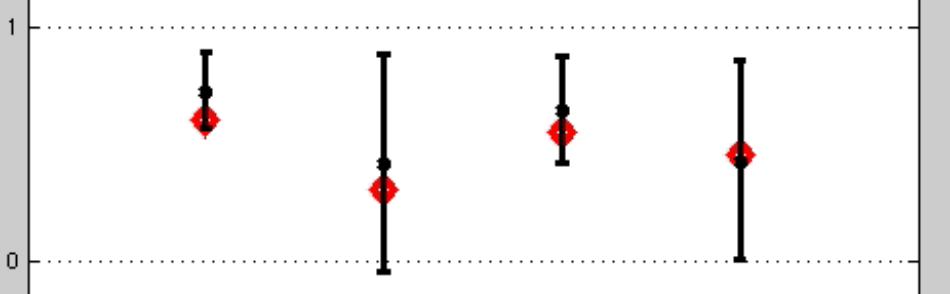
\includegraphics[width=0.55\linewidth]{UCB}
        \caption{Confidence intervals on the means after $t$ rounds}
    \end{figure}

\end{frameO}

\begin{frameO}[The optimism principle]

    \vspace{0.2cm}

    \textbf{Step 2}: act as if the best possible model were the true model

    \vspace{-0.3cm}

    \begin{center}
        \textit{
            (\textcolor{blue}{optimism in face of uncertainty})}
    \end{center}

    \vspace{-0.3cm}

    \begin{figure}
        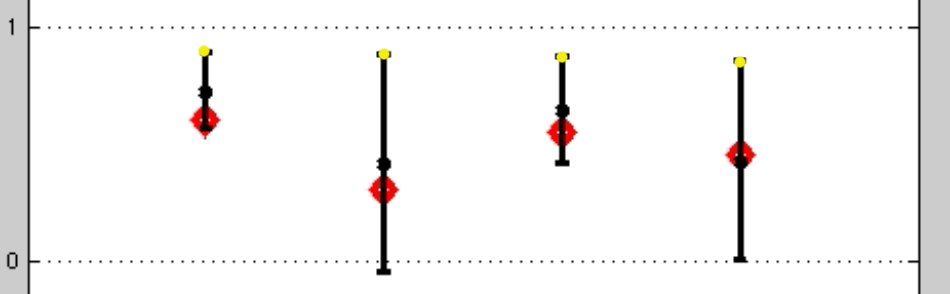
\includegraphics[width=0.55\linewidth]{UCBdot}
        \caption{Confidence intervals on the means after $t$ rounds}
    \end{figure}

    \vspace{-0.8cm}

    \[\text{Optimistic bandit model} =\argmax_{\bm\mu \in \cC(t)}  \max_{a = 1,\dots,K} \ \mu_a\]

    \vspace{-0.2cm}

    \begin{itemize}
        \item That is, select
    \end{itemize}

    \vspace{-0.4cm}

    \color{red}

    $$A_{t+1} = \underset{a=1,\dots,K}{\argmax} \ \mathrm{UCB}_a(t)\black.$$

\end{frameO}


\begin{frame}[c]
    \begin{changemargin}{-0.5cm}{-0.5cm}
        \begin{center}
            \vspace{-0.3in}
            \textbf{\huge Optimistic Algorithms}
            \vspace{1.5cm}

            {\textbf{\Large Building Confidence Intervals}	\\[0.5cm]}
            \textcolor{darkgray}{\textbf{\Large Analysis of UCB($\alpha$)}\\[0.5cm]		}
            \textcolor{darkgray}{\textbf{\Large Other UCB algorithms}\\[0.5cm]}
        \end{center}
    \end{changemargin}
\end{frame}


\begin{frameO}[How to build confidence intervals?]

    \begin{orangeblock}{}
        We need $\mathrm{UCB}_a(t)$ such that
        \[\red\bP\left(\mu_a \leq \mathrm{UCB}_a(t)\right)\gtrsim 1 - t^{-1}\black.\]

        \vspace{-0.5cm}

    \end{orangeblock}

    \vspace{-0.2cm}

    \begin{itemize}
        \item[\ding{220}] tool: \blue concentration inequalities\black
    \end{itemize}

    \textbf{Example:} rewards are \red $\sigma^2$ sub-Gaussian\black

    \vspace{-0.3cm}

    \begin{equation}\bE[Z] = \mu \ \ \text{and} \ \ \ \bE\left[e^{\lambda(Z-\mu)}\right] \leq e^{\frac{\lambda^2\sigma^2}{2}}.\label{SG}\end{equation}

    \vspace{-0.3cm}

    \begin{alertblock}{Hoeffding inequality}
        $Z_i$ i.i.d. satisfying \eqref{SG}. For all $s\geq 1$
        \[\alt<2->{\bP\left(\frac{Z_1 + \dots + Z_s}{s}  \leq \mu - x \right)  \leq e^{-\frac{sx^2}{2\sigma^2}}}{\bP\left(\frac{Z_1 + \dots + Z_s}{s}  \geq \mu + x \right)  \leq e^{-\frac{sx^2 }{2\sigma^2}}}\]
    \end{alertblock}

    \alt<3>{\color{red}\Large\danger\normalsize\black Cannot be used directly in a bandit model as \blue the number of observations from each arm is random\black!}{\vspace{-0.3cm}\begin{itemize}                                                                                                                                                             \item $\nu_a$ bounded in $[0,1]$: $1/4$ sub-Gaussian
            \item $\nu_a = \cN(\mu_a,\sigma^2)$: $\sigma^2$ sub-Gaussian                                                                                                                                                        \end{itemize}
    }


\end{frameO}

\begin{frameO}[How to build confidence intervals?]

    \vspace{0.3cm}

    \begin{itemize}
        \item $N_a(t) = \sum_{s=1}^t\ind_{(A_s = a)}$ number of selections of $a$ after $t$ rounds
        \item $\hat \mu_{a,s} = \frac{1}{s}\sum_{k=1}^s Y_{a,k}$ average of the first $s$ observations from arm $a$
        \item $\hat{\mu}_a(t) = \hat{\mu}_{a,N_a(t)}$ empirical estimate of $\mu_a$ after $t$ rounds
    \end{itemize}

    \begin{orangeblock}{Hoeffding inequality + union bound}
        $$\bP\left(\mu_a \leq \red \hat{\mu}_a(t) + \sigma\sqrt{\frac{\beta\ln(t)}{N_a(t)}} \black \right) \geq 1 - \frac{1}{t^{\frac{\beta}{2} -1}}$$
    \end{orangeblock}

    \textbf{Proof.}

    \vspace{-0.5cm}

    \begin{align*}
         & \bP\left(\mu_a > \hat{\mu}_a(t) + \sigma\sqrt{\frac{\beta\ln(t)}{N_a(t)}} \black \right) \leq  \bP\left(\exists s \leq t : \mu_a > \hat{\mu}_{a,s} + \sigma\sqrt{\frac{\beta\ln(t)}{s}} \black\right) \\
         & \leq \sum_{s=1}^t \bP\left(\hat{\mu}_{a,s} < \mu_a - \sigma\sqrt{\frac{\beta\ln(t)}{s}}\right) \leq \sum_{s=1}^t \frac{1}{t^{\beta/2}} = \frac{1}{t^{\beta/2 - 1}}.
    \end{align*}



\end{frameO}


\begin{frameO}[A first UCB algorithm]

    \vspace{0.4cm}

    UCB($\alpha$) selects  $A_{t+1} = \argmax_a \ \mathrm{UCB}_a(t)$
    where
    \[\blue \mathrm{UCB}_a(t) =\black \underbrace{\blue \hat{\mu}_{a}(t)}_{\text{exploitation term}} + \underbrace{\blue\sqrt{\frac{\alpha\ln(t)}{N_a(t)}}}_{\text{exploration bonus}}.\]

    \begin{itemize}
        \item this form of UCB was first proposed for Gaussian rewards

              \gray [Katehakis and Robbins, 95]\black
        \item popularized by \color{gray}[Auer et al. 02] \color{black} for bounded rewards: \red UCB1, for $\alpha=2$\black
        \item the analysis was UCB($\alpha$) was further refined to hold for $\alpha > 1/2$ in that case \gray [Bubeck, 11, Cappé et al. 13] \black
    \end{itemize}

\end{frameO}

\begin{frameO}[A UCB algorithm in action]

    \begin{center}
        \movie{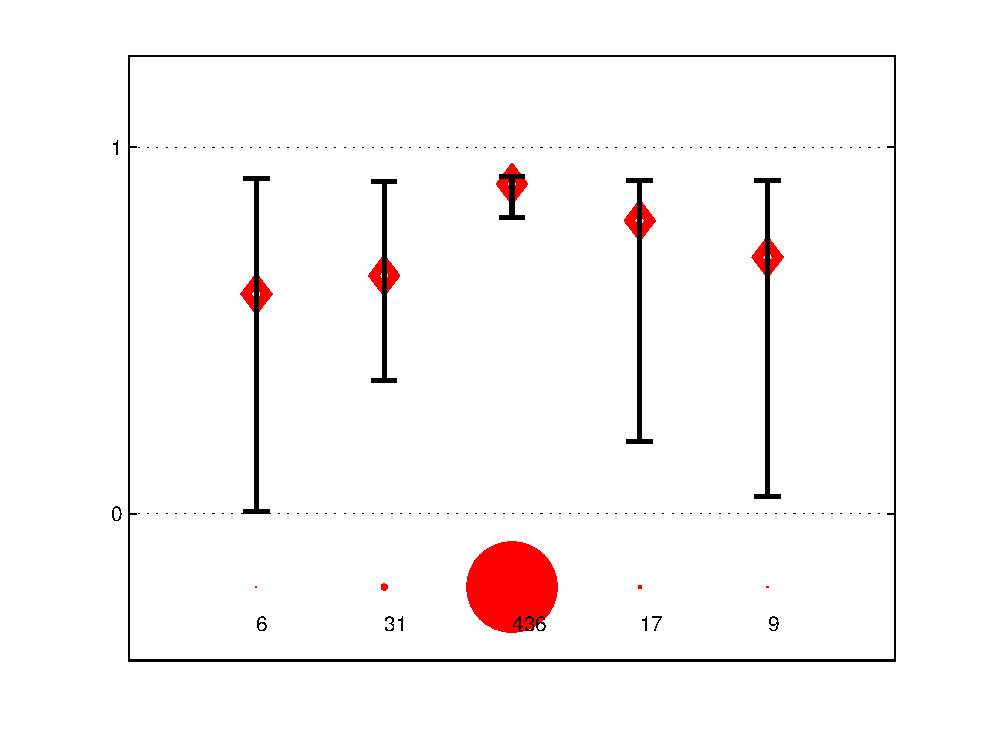
\includegraphics[width=0.9\textwidth]{KLUCB.pdf}}{KLUCB.avi}
    \end{center}
\end{frameO}


\begin{frame}[c]
    \begin{changemargin}{-0.5cm}{-0.5cm}
        \begin{center}
            \vspace{-0.3in}
            \textbf{\huge Optimistic Algorithms}
            \vspace{1.5cm}

            \textcolor{darkgray}{\textbf{\Large Building Confidence Intervals}	\\[0.5cm]}
            {\textbf{\Large Analysis of UCB($\alpha$)}\\[0.5cm]		}
            \textcolor{darkgray}{\textbf{\Large Other UCB algorithms}\\[0.5cm]}
        \end{center}
    \end{changemargin}
\end{frame}


\begin{frameO}[Regret of UCB($\alpha$) for bounded rewards]

    \vspace{0.3cm}

    \begin{orangeblock}{Theorem \gray[Auer et al, 02]\black}
        UCB($\alpha$) with parameter $\alpha=2$ satisfies

        \vspace{-0.4cm}

        \[\cR_\nu(\texttt{UCB1},T) \leq 8 \left(\sum_{a : \mu_a < \mu_\star} \frac{1}{\Delta_a}\right)\ln(T) + \left(1+\frac{\pi^2}{3}\right)\left(\sum_{a=1}^K \Delta_a\right).\]
    \end{orangeblock}

    \begin{itemize}
        \item[\ding{220}] what we will prove today
    \end{itemize}


    \begin{orangeblock}{Theorem} For every $\alpha>1$ and every sub-optimal arm $a$, there exists a constant $C_\alpha>0$ such that

        \vspace{-0.8cm}

        \[\bE_{\bm \mu}[N_a(T)] \leq \frac{4\alpha}{(\mu_\star - \mu_a)^2}\ln(T) + C_\alpha.\]
    \end{orangeblock}

    \vspace{0.2cm}

    It follows that

    \vspace{-0.6cm}

    \[\cR_\nu(\mathrm{UCB}(\alpha),T) \leq 4\alpha\blue\left(\sum_{a : \mu_a < \mu_\star}\frac{1}{\Delta_a}\right)\black\ln(T) + K C_\alpha\black.\]

\end{frameO}

\begin{frameO}[Proof : 1/3]

    \vspace{0.3cm}

    Assume $\mu_\star=\mu_1$ and $\mu_a<\mu_1$.
    \begin{eqnarray*}
        N_a(T) &=& \sum_{t=0}^{T-1}\ind_{(A_{t+1}=a)} \\
        &=&  \sum_{t=0}^{T-1}\ind_{(A_{t+1}=a)\cap(\UCB_1(t) \leq \mu_1)} + \sum_{t=0}^{T-1}\ind_{(A_{t+1}=a)\cap(\UCB_1(t) > \mu_1)} \\
        & \leq & \sum_{t=0}^{T-1}\ind_{(\UCB_1(t) \leq \mu_1)} + \sum_{t=0}^{T-1}\ind_{(A_{t+1}=a)\cap(\UCB_a(t) > \mu_1)}
    \end{eqnarray*}

    \pause

    \[\bE_\nu[N_a(T)] \leq \underbrace{\sum_{t=0}^{T-1}\bP(\UCB_1(t) \leq \mu_1)}_{A} + \underbrace{\sum_{t=0}^{T-1}\bP(A_{t+1}=a, \mathrm{UCB}_a(t) > \mu_1)}_{B} \]

\end{frameO}


\begin{frameO}[Proof : 2/3]

    \[\bE[N_a(T)] \leq \underbrace{\sum_{t=0}^{T-1}\bP(\UCB_1(t) \leq \mu_1)}_{A} + \underbrace{\sum_{t=0}^{T-1}\bP(A_{t+1}=a, \UCB_a(t) > \mu_1)}_{B} \]

    \begin{itemize}
        \item \textbf{Term A}: if $\alpha>1$,
    \end{itemize}

    \begin{eqnarray*}
        \sum_{t=0}^{T-1}\bP(\UCB_1(t) \leq \mu_1) & \leq & 1 + \sum_{t=1}^{T-1} \bP\left(\hat{\mu}_1(t) + \sqrt{\frac{\alpha \ln(t)}{N_1(t)}} \leq \mu_1\right) \\
        & \leq & 1 + \sum_{t=1}^{T-1} \frac{1}{t^{2\alpha-1}} \\
        &\leq& 1+ \zeta(2\alpha -1) :=C_\alpha/2.
    \end{eqnarray*}


\end{frameO}


\begin{frameO}[Proof : 3/3]

    %\[\bE[N_2(T)] \leq \underbrace{\sum_{t=0}^{T-1}\bP(\UCB_1(t) \leq \mu_1)}_{A} + \underbrace{\sum_{t=0}^{T-1}\bP(A_{t+1}=2, \UCB_2(t) > \mu_1)}_{B} \]

    \vspace{0.3cm}

    \begin{itemize}
        \item \textbf{Term B:}
    \end{itemize}

    \vspace{-0.6cm}

    \begin{eqnarray*}
        (B) & = &  \sum_{t=0}^{T-1}\bP\left(A_{t+1}=a, \UCB_a(t) > \mu_1\right) \\
        & \leq &  \sum_{t=0}^{T-1}\bP\left(A_{t+1}=a, \blue \UCB_a(t) > \mu_1, \mathrm{LCB}_a(t) \leq \mu_a\black\right)  + C_\alpha /2
    \end{eqnarray*}
    with

    \vspace{-0.9cm}

    \[\mathrm{LCB}_a(t) = \hat{\mu}_{a}(t) - \sqrt{\frac{\alpha \ln t}{N_a(t)}}.\]


    \begin{columns}
        \begin{column}{5.5cm}
            $\blue\mu_1,\mu_a \in \left[\mathrm{LCB}_a(t) ; \UCB_a(t)\right]$
            \begin{eqnarray*}
                &\Rightarrow &(\mu_1 - \mu_a) \leq 2 \sqrt{\frac{\alpha \ln(T)}{N_a(t)}} \\
                & \Rightarrow & \ N_a(t) \leq \frac{4\alpha}{(\mu_1 - \mu_a)^2}\ln(T)
            \end{eqnarray*}
        \end{column}
        \begin{column}{4.5cm}
            \begin{center}
                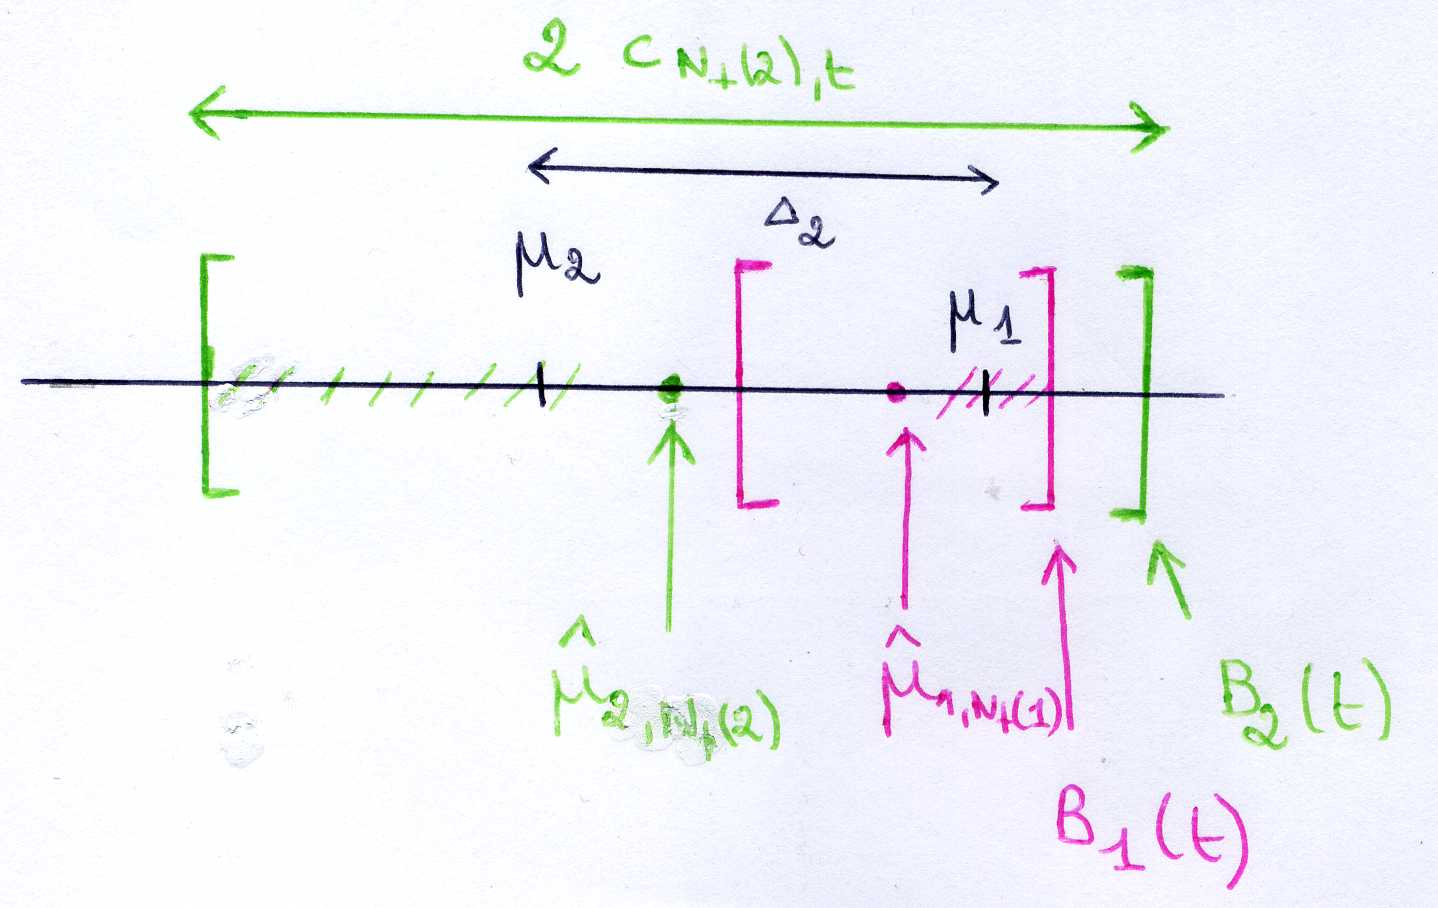
\includegraphics[height=2.7cm]{illUCB.jpg}
            \end{center}
        \end{column}
    \end{columns}




\end{frameO}

\begin{frameO}[Proof : 3/3]

    %\[\bE[N_2(T)] \leq \underbrace{\sum_{t=0}^{T-1}\bP(\UCB_1(t) \leq \mu_1)}_{A} + \underbrace{\sum_{t=0}^{T-1}\bP(A_{t+1}=2, \UCB_2(t) > \mu_1)}_{B} \]

    \begin{itemize}
        \item \textbf{Term B:} (continued)
    \end{itemize}

    \vspace{-0.3cm}

    \begin{eqnarray*}
        (B) & \leq &  \sum_{t=0}^{T-1}\bP(A_{t+1}=a, \UCB_a(t) > \mu_1, \text{LCB}_a(t) \leq \mu_a) %\\ && \hspace{1.3cm} + \hspace{0.3cm} \sum_{t=0}^{T-1}\bP(\UCB_2(t) \leq \mu_2)
        + C_\alpha /2 \\
        & \leq &  \sum_{t=0}^{T-1}\bP\left(A_{t+1}=a, N_a(t) \leq \frac{4\alpha}{(\mu_1 - \mu_a)^2}\ln(T)\right)+ C_{\alpha}/2 \\
        & \leq & \frac{4\alpha}{(\mu_1 - \mu_a)^2}\ln(T) + C_\alpha/2
    \end{eqnarray*}


    \begin{itemize}
        \item \textbf{Conclusion}:
    \end{itemize}

    \[\bE[N_a(T) ] \leq \frac{4\alpha}{(\mu_1 - \mu_a)^2}\ln(T) + C_\alpha.\]


\end{frameO}


\begin{frameO}[An improved analysis]

    \alt<3>{\vspace{0.4cm}}{\vspace{0.3cm}}

    \textbf{Context:} $\sigma^2$ sub-Gaussian rewards

    \vspace{-0.2cm}

    \[\UCB_a(t) = \hat{\mu}_a(t) + \sqrt{\frac{2\sigma^2(\ln(t) + c\ln\ln(t))}{N_a(t)}}\]

    \vspace{-0.2cm}

    \begin{orangeblock}{Theorem \color{gray}[Cappé et al.'13]}
        For $c \geq 3$, the UCB algorithm associated to the above index satisfy
        \[\bE[N_a(T)] \leq \frac{2\sigma^2}{(\mu_\star - \mu_a)^2}\ln(T) + C_{\bm\mu}\sqrt{\ln(T)}.\]
    \end{orangeblock}

    \pause

    \alt<4>{\vspace{-0.3cm}}{}

    \alt<4>{
        \begin{itemize}
            \item \underline{Bernoulli rewards:}

                  \vspace{-0.3cm}

                  \[\mathcal{R}_{\nu}(\mathrm{UCB},T) \neq\red \left(\sum_{a : \mu_a < \mu_\star} \frac{\Delta_a}{\kl(\mu_a,\mu_\star)}\right)\black \ln(T) \]

                  \vspace{-0.3cm}

            \item[\ding{220}] \red not \black matching the Lai and Robbins lower bound

                  \underline{Pinsker's inequality}: $\blue 2 \Delta_a^2 \leq \kl(\mu_a,\mu_\star)$.
        \end{itemize}}{
        \alt<3>{
            \begin{itemize}
                \item \underline{Bernoulli rewards:}

                      \vspace{-0.3cm}

                      \[\mathcal{R}_{\nu}(\mathrm{UCB},T) \lesssim\blue \left(\sum_{a : \mu_a < \mu_\star} \frac{1}{2\Delta_a}\right)\black \ln(T) \]

                      \vspace{-0.3cm}

                \item[\ding{220}] optimal ?
            \end{itemize}
        }
        {\begin{itemize}
                \item \underline{Gaussian rewards:}

                      \vspace{-0.3cm}

                      \[\mathcal{R}_{\nu}(\mathrm{UCB},T) \lesssim \blue \left(\sum_{a : \mu_a < \mu_\star} \frac{2\sigma^2}{\Delta_a}\right)\black \ln(T) .\]

                      \vspace{-0.3cm}

                \item[\ding{220}] matching the Lai and Robbins lower bound! \blue asymptotically optimal \black
            \end{itemize}}}



\end{frameO}



\begin{frameO}[The Worst--case Performance of UCB]
    \begin{itemize}
        \item UCB worst-case regret:  $O(\blue\sqrt{KT \ln(T)})$
    \end{itemize}
    \begin{eqnarray*}
        \cR_\nu(\texttt{UCB},T) & = &\sum_{a=1}^K \textcolor{red}{\Delta_a\sqrt{\bE[N_a(T)]}}\sqrt{\bE[N_a(T)]} \\
        &=&\sum_{a=1}^K O(\red{\sqrt{\ln(T)}}\black)\sqrt{\bE[N_a(T)]}\\
        &\leq& K\sqrt{\frac{1}{K} \sum_{a}\bE[N_a(T)]}O(\sqrt{\ln(T)})\\
        &=& O(\sqrt{KT \ln(T)})
    \end{eqnarray*}
    \begin{itemize}
        \item[\ding{220}] not exactly matching the $\blue\sqrt{KT}$ lower bound...
    \end{itemize}

\end{frameO}



\begin{frame}[c]
    \begin{changemargin}{-0.5cm}{-0.5cm}
        \begin{center}
            \vspace{-0.3in}
            \textbf{\huge Optimistic Algorithms}
            \vspace{1.5cm}

            \textcolor{darkgray}{\textbf{\Large Building Confidence Intervals}	\\[0.5cm]}
            \textcolor{darkgray}{\textbf{\Large Analysis of UCB($\alpha$)}\\[0.5cm]		}
            {\textbf{\Large Other UCB algorithms}\\[0.5cm]}
        \end{center}
    \end{changemargin}
\end{frame}

\begin{frameO}[UCB-V]

    UCB with empirical \red V\black ariance estimates \gray [Audibert et al. 09] \black selects
    \[A_{t+1} = \argmax_{a=1,\dots,K} \ \red  \hat\mu_{a}(t) + \sqrt{\frac{2{\hat{\sigma}_a(t)} \ln t^3}{N_a(t)}} + \frac{7\ln t^3}{3{N_a(t)}}\]
    where $\hat{\sigma}_a(t) =\frac{1}{N_a(t)}\sum_{s=1}^{N_a(t)} \left(Y_{a,s} - \hat{\mu}_a(t)\right)^2$.

    \vspace{0.3cm}

    \alt<2>{\begin{orangeblock}{Theorem \gray[Audibert et al. 09]}
            For a bandit instance with bounded rewards, UCB-V satisfies
            \[\cR_\nu\left(\texttt{UCB-V},T\right) \leq C \blue\left(\sum_{a : \mu_a < \mu_\star}\frac{\sigma_a^2}{\Delta_a}\right)\black\ln(T)\]

            \vspace{-0.3cm}

            for some constant $C$.
        \end{orangeblock}
    }{
        \begin{alertblock}{Empirical Bernstein Inequality}
            Let $X_i\in[0,1]$ be $n$ {independent} r.v. with mean $\mu_i = \bE X_i$ and {variance} $\sigma^2$
            \begin{equation*}
                \bP\Big(\frac{1}{n}\sum_{i=1}^n \big(X_i - \mu_i\big)  \geq \sqrt{\frac{2\hat \sigma_n^2\ln(2/\delta)}{n}} + \frac{7\ln(2/\delta)}{3n}\Big) \leq \delta
            \end{equation*}

            \vspace{-0.3cm}

            where $\hat \sigma_n^2$ is the \blue empirical variance estimate\black.
        \end{alertblock}

    }

\end{frameO}

\begin{frameO}[UCB for Gaussian distributions]

    $\nu_a = \cN(\mu_a, \sigma_a^2)$ with \blue unknown mean AND variance \black.

    \begin{orangeblock}{ISM-Normal \color{gray} [Cowan et al. 17] \black}
        \[A_{t+1} = \argmax_{a=1,\dots,K} \ \red \hat{\mu}_a(t) + \hat{\sigma}_a(t) \sqrt{t^{\frac{2}{N_a(t) -2}}-1}\black.\]
    \end{orangeblock}

    \begin{itemize}
        \item an \blue asymptotically optimal \black algorithm
    \end{itemize}

    \vspace{-0.4cm}

    \[\cR_{\nu}(\texttt{ISM},T) \leq (1+\varepsilon)\!\!\!\!\!\!\!\!\underbrace{\blue\sum_{a : \mu_a < \mu_\star} \frac{2}{\ln\left(1+ \frac{\Delta_a^2}{\sigma_a^2}\right)}\black}_{\substack{\text{optimal constant}\\\text{(Burnetas and Katehakis lower bound)}}}\!\!\!\!\!\!\!\!\ln(T) + O_\varepsilon(\ln\ln(T)).\]

    \begin{itemize}
        \item[\ding{220}] asymptotic optimality beyond Gaussian rewards?
    \end{itemize}

\end{frameO}


\begin{frameTI}
    \begin{center}
        \color{white} \Huge \textsc{Asymptotically optimal}

        \textsc{algorithms}
    \end{center}
    \vspace*{-4pt}
\end{frameTI}

\begin{frameO}[The idea of \klUCB{}]

    \vspace{0.4cm}

    \textbf{Context:} $\nu_1,\dots,\nu_K$ belong to a \blue one-dimensional exponential family\black:
    \[\cP_{\eta,\Theta,b}=\{\nu_{\theta}, \theta \in \Theta : \nu_{\theta} \ \text{has density} \ f_{\theta}(x)=\exp(\theta x - b(\theta)) \ w.r.t. \ \eta\}\]

    \vspace{-0.3cm}

    \begin{itemize}
        \item $\nu_{\theta}$ can be parameterized by its mean $\blue\mu = \dot{b}(\theta)\black$ : $\red \nu^\mu := \nu_{\dot{b}^{-1}(\mu)}\black$
        \item $\nu \leftrightarrow \bm\mu = (\mu_1,\dots,\mu_K)$
    \end{itemize}
    \textbf{Example:} \textit{Bernoulli, Gaussian with known variance, Poisson, Exponential}
    \vspace{0.3cm}

    \textbf{Lai and Robbins lower bound:}
    \[\liminf_{T\rightarrow \infty} \frac{\cR_\nu(\cA,T)}{\ln(T)} \geq \sum_{a : \mu_a < \mu_\star} \frac{\Delta_a}{\red\kl\black(\mu_a,\mu_\star)}.\]

    \textbf{Idea:} algorithms exploiting the KL-divergence associated to that exponential family
    \[\red \kl(\mu,\mu') = \KL\left(\nu^\mu,\nu^{\mu'}\right)\black.\]

\end{frameO}

\begin{frameO}[The $\mathrm{kl}$-UCB index]

    \begin{orangeblock}{}
        Fix an exponential family and its divergence function $\kl(\mu,\mu')$.
        \[\UCB_{a}(t)=\max\left\{q : \red \kl\black\left(\hat{\mu}_a(t),q\right) \leq \frac{\ln(t)+c\ln\ln(t)}{N_a(t)}\right\},
        \]
        for some parameter $c\geq 0$.
    \end{orangeblock}

    \vspace{-0.5cm}

    \begin{center}
        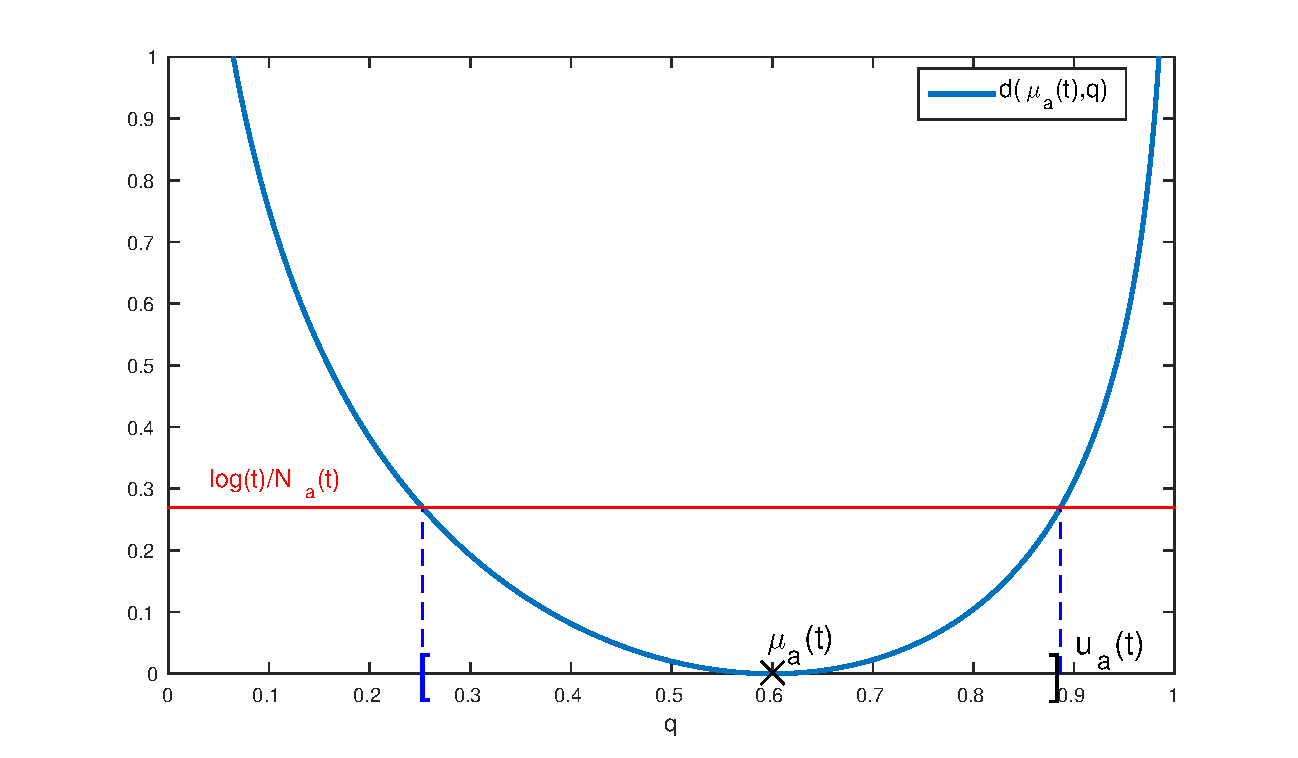
\includegraphics[height=3.5cm]{Interval.pdf}
    \end{center}

    \vspace{-0.4cm}

    {\small
        \gray [Lai, 1987] \black: first occurence of a kl-UCB index (asymptotic analysis)

        \gray [Garivier and Cappé, 2011] [Cappé, Garivier, Maillard, Munos, Stoltz, 2013] \black : non-asymptotic analysis of kl-UCB for exponential families}

\end{frameO}

\begin{frameO}[Why is it a UCB?]

    \begin{orangeblock}{}
        Fix an exponential family and its divergence function $\kl(\mu,\mu')$.
        \[\UCB_{a}(t)=\max\left\{q : \red \kl\black\left(\hat{\mu}_a(t),q\right) \leq \frac{\ln(t)+c\ln\ln(t)}{N_a(t)}\right\},
        \]

        \vspace{-0.3cm}

        for some parameter $c\geq 0$.
    \end{orangeblock}

    \alt<3>{\textbf{General case}: follows from
        \begin{alertblock}{Chernoff inequality for exponential families}
            $Z_i$ i.i.d. and $Z_1 \sim \nu^{\mu}$. For all $s\geq 1$
            \[\forall u < \mu, \ \ \bP\left(\frac{Z_1 + \dots + Z_s}{s}  \leq u \right)  \leq e^{-s\times\red\kl\black(u,\mu)}\]
        \end{alertblock}

        \color{red}\Large\danger\normalsize\black Cannot be used directly in a bandit model as \blue the number of observations from each arm is random\black!
    }{\alt<2>{\textbf{General case}: follows from
            \begin{alertblock}{Chernoff inequality for exponential families}
                $Z_i$ i.i.d. and $Z_1 \sim \nu^{\mu}$. For all $s\geq 1$
                \[\forall u > \mu, \ \ \bP\left(\frac{Z_1 + \dots + Z_s}{s}  \geq u \right)  \leq e^{-s\times\red\kl\black(u,\mu)}\]
            \end{alertblock}

            \color{red}\Large\danger\normalsize\black Cannot be used directly in a bandit model as \blue the number of observations from each arm is random\black!
        }{\textbf{Gaussian bandit}: \[\kl(\mu,\mu') = \frac{(\mu - \mu')^2}{2\sigma^2}\]
            We recover
            \[\blue\UCB_a(t) = \hat{\mu}_a(t) + \sqrt{\frac{2\sigma^2\left(\ln(t) + c \ln\ln(t)\right)}{N_a(t)}}\black\]
            \begin{itemize}
                \item[\ding{220}] upper-confidence bound on $\mu_a$
            \end{itemize}

        }}

    % \begin{eqnarray*}
    %  \bP\left(\mu_a > \UCB_{a,s}(\gamma) \right) & = & \bP\left(s\times \kl(\hat{\mu}_{a,s} , \mu_a) > \gamma)\right) \\
    %  & = & \bP\left(\hat{\mu}_{a,s} > x_\gamma\right) \leq e^{-sd(x_\gamma,\mu)} = e^{-\gamma}
    % \end{eqnarray*}
    % where $x_\gamma$ is such that $s \times \kl(x_\gamma,\mu) = \gamma$.{\alt<2>{\textbf{General case}: follows from


\end{frameO}



\begin{frameO}[An asymptotically optimal algorithm]

    \vspace{0.3cm}

    \klUCB{} selects $A_{t+1} = \argmax_{a} \UCB_a(t)$ with
    \[\UCB_{a}(t)=\max\left\{q : \red \kl\black\left(\hat{\mu}_a(t),q\right) \leq \frac{\ln(t)+c\ln\ln(t)}{N_a(t)}\right\}.
    \]

    \vspace{-0.3cm}

    \begin{orangeblock}{Theorem \gray[Cappé et al, 13]} If $c \geq 3$, for every arm such that $\mu_a < \mu_\star$,
        \[\bE_{\bm\mu}[N_a(T)] \leq \frac{1}{\red\kl\black(\mu_a,\mu_\star)}\ln(T) + C_{\bm\mu}\sqrt{\ln(T)}.\]
        \begin{center}
            \textit{(explicit constant in the paper)}
        \end{center}
    \end{orangeblock}

    \begin{itemize}
        \item \blue asymptotically optimal \black for rewards in a 1-d exponential family:
    \end{itemize}
    \[\cR_{\bm\mu}(\mathrm{kl}\text{-UCB},T) \simeq \blue \left(\sum_{a : \mu_a < \mu_\star} \frac{\Delta_a}{\kl(\mu_a,\mu_\star)}\right)\black\ln(T).\]



\end{frameO}

\begin{frameO}[UCB versus kl-UCB]

    \vspace{0.3cm}

    \[\bm\mu = [0.1 \ 0.05 \ 0.05 \ 0.05 \ 0.02 \ 0.02 \ 0.02 \ 0.01 \ 0.01 \ 0.01]\]

    \vspace{-0.5cm}

    \begin{center}
        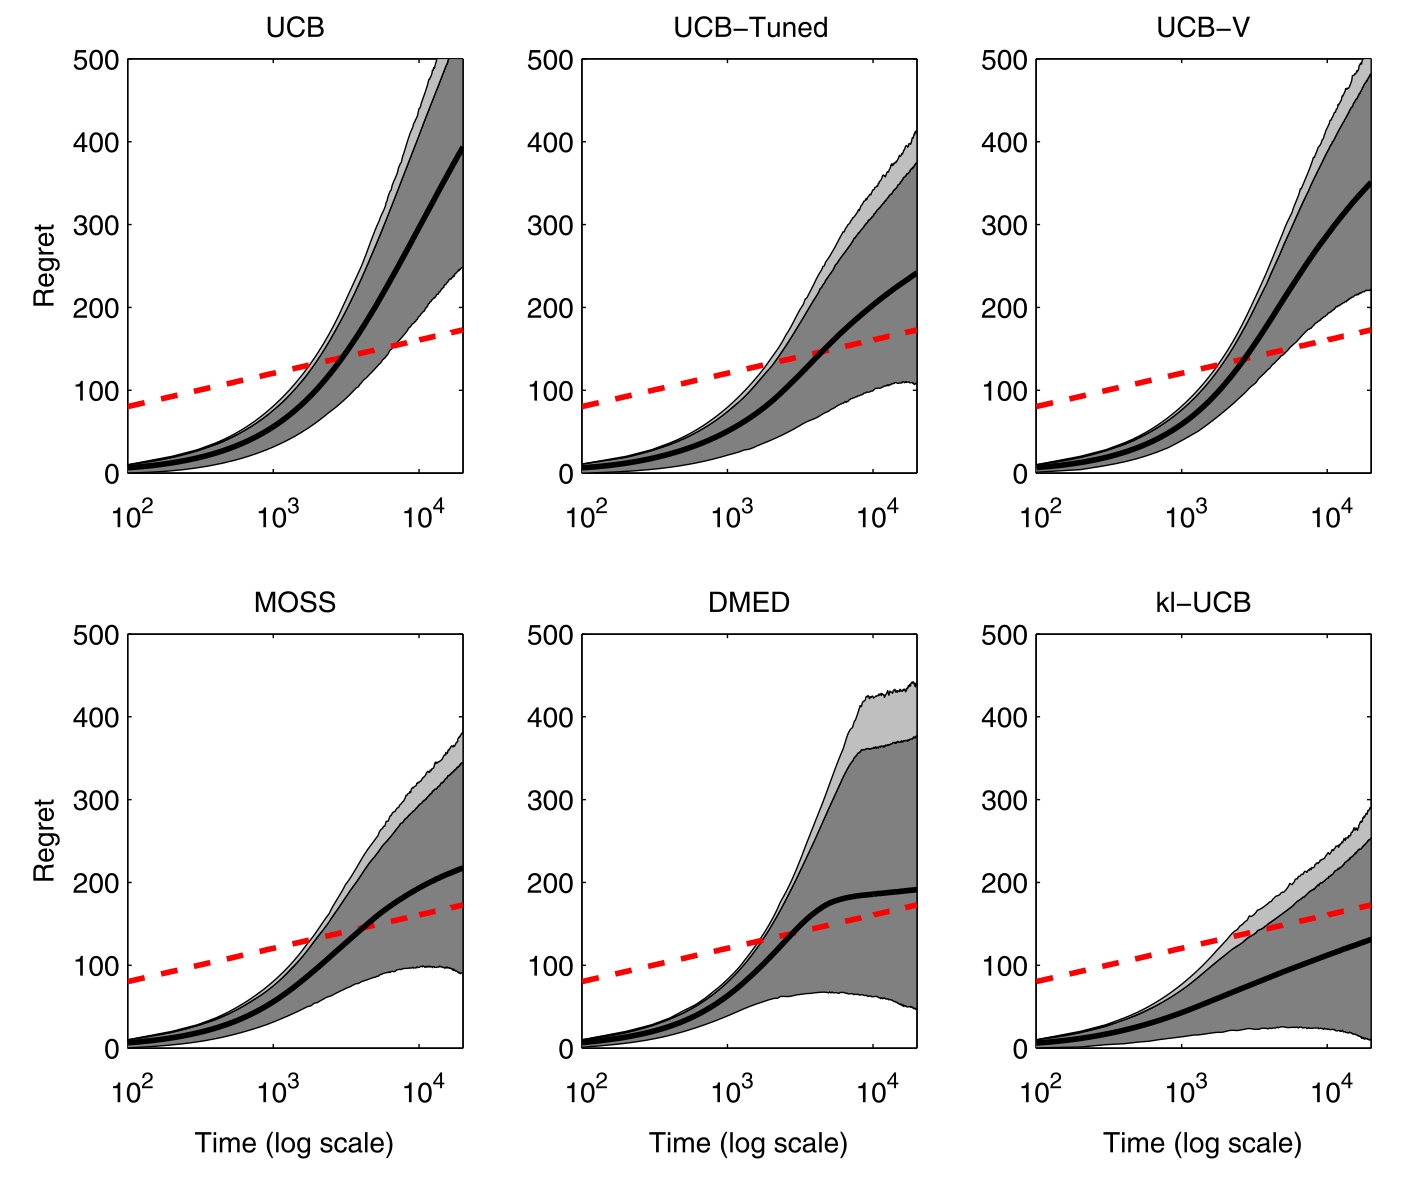
\includegraphics[width=0.7\textwidth]{curves_klUCB}
    \end{center}

    \vspace{-0.6cm}

    \hfill {\small (Credit: Cappé et al.)}
\end{frameO}

\begin{frameO}[Where do the improvements come from?]

    \begin{orangeblock}{Theorem \gray[Cappé et al, 13]} If $c \geq 3$, for every arm such that $\mu_a < \mu_\star$,
        \[\bE_{\bm\mu}[N_a(T)] \leq \frac{1}{\kl(\mu_a,\mu_\star)}\ln(T) + C_{\bm\mu}\sqrt{\ln(T)}.\]
        \begin{center}
            \textit{(explicit constant in the paper)}
        \end{center}
    \end{orangeblock}

    \begin{itemize}
        \item[\ding{220}] follows from  \red two improvements \black in the previous analysis
    \end{itemize}
    \alt<3>{\[\bE[N_a(T)] \leq \underbrace{\sum_{t=0}^{T-1}\bP(\UCB_1(t) \leq \mu_1)}_{A : \blue \text{ a better concentration result}} + \underbrace{\frac{f(T)}{\kl(\mu_a,\mu_1)} + O(\sqrt{f(T)})}_{B : \red\text{ a finer upper bound}} \]}
    {\alt<2>{\[\bE[N_a(T)] \leq \underbrace{\sum_{t=0}^{T-1}\bP(\UCB_1(t) \leq \mu_1)}_{A : \red\text{ a better concentration result}} + \underbrace{\sum_{s=1}^{T}\bP(s\times \kl(\hat\mu_{a,s} , \mu_1) \leq f(T))}_{B : \red \text{ a finer upper bound}} \]
        }{\[\bE[N_a(T)] \leq \underbrace{\sum_{t=0}^{T-1}\bP(\UCB_1(t) \leq \mu_1)}_{A : \red \text{ a better concentration result}} + \underbrace{\sum_{t=0}^{T-1}\bP(A_{t+1}=a, \UCB_a(t) > \mu_1)}_{B : \red \text{ a finer upper bound}} \]}}

    \alt<2->{\hfill$f(T) = \ln(T) + c \ln\ln(T)$}{}
\end{frameO}


\begin{frameO}[Self-normalized concentration inequalities]

    \begin{eqnarray*}
        \bP(\UCB_1(t) \leq \mu_1) & = & \bP\left( N_1(t)\times \kl^+\!\!\left(\hat{\mu}_1(t),\mu_1\right) > \ln(t) + c\ln\ln(t)\right) \\
        & \leq & \bP\left(\exists s \leq t : s \times \kl^+(\hat{\mu}_{1,s},\mu_1) > \ln(t) + c\ln\ln(t)\right)
    \end{eqnarray*}

    \alt<3>{\textbf{Second idea:} \red peeling trick \black
    \begin{alertblock}{Lemma \gray[Garivier and Cappé, 2011]}
        \[\bP\left(\exists s \leq t : s \times \kl^+\left(\hat{\mu}_{1,s},\mu_1\right) > \gamma \right) \leq e \lceil\gamma \ln(t)\rceil  e^{-\gamma}.\]
    \end{alertblock}

    \vspace{-0.3cm}

    \begin{eqnarray*}
        \bP(\UCB_1(t) \leq \mu_1) & = & O\left( \frac{\ln^2(t)}{t\ln^c(t)}\right)
    \end{eqnarray*}

    \[\rightsquigarrow \red  \sum_{t=1}^\infty
        \bP(\UCB_1(t) \leq \mu_1) < \infty \black \ \ \ \text{for } c \geq 3.\]


    }{
    \alt<2>{\textbf{Second idea:} \red peeling trick \black

    \vspace{0.3cm}

    Introducing \blue slices $\cI_k = \{t_{k}, \dots,t_{k+1}\}$\black, with $t_k = \lfloor (1+\eta)^{k-1}\rfloor$.
    \begin{align*}
        \hspace{-0.4cm}\bP(\UCB_1(t) \leq \mu_1) & \!\leq\!\!\sum_{k=1}^{\frac{\ln(t)}{\ln(1+\eta)}} \bP\left( \exists s \in \cI_k , s\times \kl^+\!\!\left(\hat{\mu}_{1,s},\mu_1\right)\! > \!\ln(t) + c\ln\ln(t)\right)                                                                                             \\
                                                 & \leq \!\!  \sum_{k=1}^{\frac{\ln(t)}{\ln(1+\eta)}} \underbrace{\bP\left( \exists s \in \cI_k , s\times \kl^+\!\!\left(\hat{\mu}_{1,s},\mu_1\right)\! > \!\ln(t_{k}) + c\ln\ln(t_{k})\right)}_{\substack{\text{deviation of } \hat{\mu}_{1,s} \text{ from its mean} \\\ \blue \text{uniformly over } s\in\cI_k}} \\
    \end{align*}

    \vspace{-1cm}

    \[\hspace{4cm} \rightsquigarrow \red  \text{maximal inequalities for martingales}\]
    }{
    \textbf{First idea:} union bound + Chernoff inequality
    \begin{eqnarray*}
        \bP(\UCB_1(t) \leq \mu_1) & = & \sum_{s=1}^t \bP\left( s\times \kl^+\!\!\left(\hat{\mu}_{1,s},\mu_1\right) > \ln(t) + c\ln\ln(t)\right) \\
        & \leq & \sum_{s=1}^t \frac{1}{t\ln^c(t)} = \frac{1}{\ln(t)^c}
    \end{eqnarray*}

    \[\rightsquigarrow \red  \sum_{t=1}^\infty \bP(\UCB_1(t) < \mu_1) = \infty\]
    \begin{itemize}
        \item[\ding{220}] not good enough...
    \end{itemize}

    }}

\end{frameO}

\begin{frameO}[\klUCB{} beyond exponential families]

    \begin{itemize}
        \item \klUCB{} \blue can be used for arbitrary rewards in $[0,1]$ \black with
              \begin{itemize}
                  \item[\ding{220}] the Gaussian divergence $\kl(x,y) = 2(x-y)^2$ (UCB)
                  \item[\ding{220}] the Bernoulli divergence $\kl(x,y) = \KL(\cB(x),\cB(y))$
              \end{itemize}
              with the same theoretical guarantees. \hfill \gray[Cappé et al. 13]\black

    \end{itemize}

    \begin{itemize}
        \item variants of kl-UCB for \blue other types of parametric reward distributions \black
              \begin{itemize}
                  \item[\ding{220}] distribution with a finite support \hfill \gray[Maillard et al. 11][Cappé et al. 13]\black

                  \item[\ding{220}] exponential family with $d > 1$ parameters \hfill  \gray [Maillard, 17]
              \end{itemize}
    \end{itemize}

    \begin{itemize}
        \item variants that \blue do not exploit parametric assumptions \black that obtain better guarantees for arbitrary rewards
              \begin{itemize}
                  \item[\ding{220}] DMED, IMED \hfill \gray [Honda and Takemura, 10][Honda and Takemura, 16] \black
                  \item[\ding{220}] empirical KL-UCB for bounded rewards \hfill \gray[Cappé et al. 13]\black
              \end{itemize}
    \end{itemize}

\end{frameO}



%
% {\vspace{-0.5cm}
%
%  \[\color{gray} \text{[Cappé et al. 13]}\black: \ \ \ \bE_{\bm \mu}[N_k(T)]\leq  \color{blue}\frac{1}{d(\mu_k,\mu_\star)}\color{black}{\ln T} + O(\sqrt{\ln(T)}).\]}

\begin{frameTI}
    \begin{center}
        {\textcolor{white} {\Huge \textsc{Worst-case Optimality} }}
    \end{center}
    \vspace*{-4pt}
\end{frameTI}


\begin{frameO}[The MOSS algorithm]

    \vspace{0.3cm}

    \red M\black inimax \red O\black ptimal \red S\black trategy in the \red S\black tochastic case.

    \gray [Audibert and Bubeck, 09] \black

    \vspace{-0.5cm}

    \[A_{t+1} = \argmax_{a = 1,\dots,K} \ \red \hat{\mu}_a(t) + \sqrt{\frac{\ln_+\left(\frac{T}{KN_a(t)}\right)}{N_a(t)}}\]

    \begin{orangeblock}{Theorem \gray [Audibert and Bubeck, 09]}
        Let $\nu$ be a bandit instance with bounded rewards.
        \begin{enumerate}
            \item Letting $\Delta_{\min} = \underset{a : \mu_a < \mu_\star}{\mathrm{min}} (\mu_\star - \mu_a)$,

                  \vspace{-0.2cm}

                  \[\cR_\nu(\texttt{MOSS},T) \leq \alt<2>{\blue\frac{23K}{\Delta_{\min}}\black}{\frac{23K}{\Delta_{\min}}}\ln\left(\max\left[\frac{110T\red\Delta_{\min}^2\black}{K},10^4\right]\right).\]\alt<2>{\vspace{-0.2cm}}{}
            \item It also holds that $\cR_\nu(\texttt{MOSS},T) \leq 25\red \sqrt{KT}\black$.

        \end{enumerate}


    \end{orangeblock}

    \alt<2>{\begin{itemize}
            \item[\ding{220}] \blue far from optimal \black in a problem-dependent sense
        \end{itemize}}{
        \begin{itemize}
            \item[\ding{220}] matching the worse-case lower bound!
        \end{itemize}}



\end{frameO}

\begin{frameO}[KL-UCB switch]

    \vspace{0.3cm}

    \textbf{Idea:} ``switch'' between KL-UCB and MOSS in order to be simultaneously \blue optimal \black in a problem-dependent and worse-case sense.

    \hfill\gray [Garivier et al., 2018]\black

    KL-UCB switch is the index policy associated to
    \[\red\UCB_a(t) = \left\{\begin{array}{cl}
            \UCB_a^{\text{KL}}(t) & \text{if } N_a(t) \leq (T/K)^{1/5},          \\
            \UCB_a^{\text{M}}(t)  & \text{if } N_a(t) > (T/K)^{1/5}\alt<2>{.}{,} \\
        \end{array}\right.\]

    \vspace{-0.3cm}

    \alt<2>{\begin{orangeblock}{Theorem \gray [Garivier et al. 18]}
            Fix $\nu$ a bandit instance with bounded rewards.
            \begin{enumerate}
                \item For all sub-optimal arm $a$,
                      \[\bE_{\nu}[N_a(T)] \leq \blue\frac{\ln(T)}{\kl(\mu_a,\mu_\star)}\black + O\left(\ln^{2/3}(T)\right)\]
                \item Moreover, $\cR_\nu(\text{KL-UCB-Switch},T) \leq 25\blue\sqrt{KT}\black + (K-1)$.
            \end{enumerate}
        \end{orangeblock}}{where \begin{orangeblock}{}\vspace{-0.3cm}
            \begin{eqnarray*}
                \UCB_a^{\text{KL}}(t)& = & \max \left\{ q : N_a(t) \times \kl\left(\hat{\mu}_a(t), q\right) \leq \ln_+\left(\blue\frac{T}{KN_a(t)}\black\right) \right\}\footnote{$\kl(x,y)=\kl_{\text{Ber}}(x,y)$; \text{can also rely on the non-parameteric KL-UCB index}},\\
                \UCB_a^{\text{M}}(t)& = &\hat{\mu}_a(t) + \sqrt{\frac{\ln_+\left(\blue\frac{T}{KN_a(t)}\black\right)}{2N_a(t)}}.
            \end{eqnarray*}\end{orangeblock}}




\end{frameO}

\begin{frameO}[Intermediate Summary]

    \begin{itemize}
        \item Several ways to solve the exploration/exploitation trade-off
              \begin{itemize}
                  \item Explore-Then-Commit
                  \item $\varepsilon$\texttt{-greedy}
                  \item \red Upper Confidence Bound algorithms \black
              \end{itemize}
    \end{itemize}

    \begin{itemize}
        \item Good concentration inequalities are crucial to build good UCB algorithms!
    \end{itemize}

    \begin{itemize}
        \item Performance lower bounds motivate the design of (optimal) algorithms
    \end{itemize}

\end{frameO}

\begin{frameTI}
    \begin{center}
        {\textcolor{white} {\Huge \textsc{A Bayesian Look at the Multi-Armed Bandit Model} }}
    \end{center}
    \vspace*{-4pt}
\end{frameTI}


\begin{frameO}[Historical perspective]


    \begin{minipage}{0.04\textwidth}\hspace{0.5cm}\end{minipage}\begin{minipage}{0.95\textwidth}{\footnotesize\begin{itemize}
                \item[]
                \item[1952] Robbins, formulation of the MAB problem
                \item[]
                \item[]
                \item[1985] Lai and Robbins: lower bound, first asymptotically optimal algorithm
                \item[]
                \item[1987] Lai, asymptotic regret of \klUCB{}
                \item[1995] Agrawal, UCB algorithms
                \item[1995] Katehakis and Robbins, a UCB algorithm for Gaussian bandits
                \item[2002] Auer et al: UCB1 with finite-time regret bound
                \item[2009] UCB-V, MOSS...
                \item[]
                \item[2011,13] Cappé et al: finite-time regret bound for \klUCB{}
                \item[]
            \end{itemize}}
    \end{minipage}


\end{frameO}

\begin{frameO}[Historical perspective]


    \begin{minipage}{0.04\textwidth}\hspace{0.5cm}\end{minipage}\begin{minipage}{0.95\textwidth}{\footnotesize\begin{itemize}
                \item[1933] \blue Thompson: a Bayesian mechanism for clinical trials\black
                \item[1952] Robbins, formulation of the MAB problem
                \item[1956] \blue Bradt et al, Bellman: optimal solution of a Bayesian MAB problem \black
                \item[1979] \blue Gittins: first Bayesian index policy \black
                \item[1985] Lai and Robbins: lower bound, first asymptocally optimal algorithm
                \item[1985] \blue Berry and Fristedt: Bandit Problems, a survey on the Bayesian MAB \black
                \item[1987] Lai, asymptotic regret of \klUCB{} \blue + study of its Bayesian regret\black
                \item[1995] Agrawal, UCB algorithms
                \item[1995] Katehakis and Robbins, a UCB algorithm for Gaussian bandits
                \item[2002] Auer et al: UCB1 with finite-time regret bound
                \item[2009] UCB-V, MOSS...
                \item[2010] \blue Thompson Sampling is re-discovered \black
                \item[2011,13] Cappé et al: finite-time regret bound for \klUCB{}
                \item[2012,13] \blue Thompson Sampling is asymptotically optimal\black
            \end{itemize}}
    \end{minipage}


\end{frameO}


\begin{frameO}[Frequentist versus Bayesian bandit]

    \vspace{0.4cm}

    $\nu_{\bm \mu}=(\nu^{\mu_1},\dots,\nu^{\mu_K}) \in (\cP)^K$.

    \vspace{0.2cm}

    \begin{itemize}
        \item Two probabilistic models
    \end{itemize}

    \begin{center}
        \begin{tabular}{|c|c|}
            \hline
            \textbf{\red Frequentist\color{black} \ model}                             & \textbf{\red Bayesian\color{black} \ model}                                         \\
            \hline
            $\mu_1,\dots,\mu_K$                                                        & $\mu_1,\dots,\mu_K$ drawn from a                                                    \\
            \hspace{0.7cm}\red unknown parameters\color{black} \hspace{0.7cm}          & \red prior distribution \color{black}: ${\mu_a} \ {\sim} \ \pi_a$                   \\
            \hline
            \text{arm} \ $a$: \ $(Y_{a,s})_s \overset{\text{i.i.d.}}{\sim}\nu^{\mu_a}$ & \text{arm} \ $a$: $(Y_{a,s})_s | \bm{\mu} \overset{\text{i.i.d.}}{\sim}\nu^{\mu_a}$ \\
            \hline
        \end{tabular}
    \end{center}

    \vspace{0.2cm}

    % Y is the sequence of successive rewards obtained from arm a...

    \begin{itemize}
        \item The regret can be computed in each case % giving two measures of performance
    \end{itemize}

    \vspace{-0.2cm}

    \begin{center}
        \begin{tabular}{c|c}
            Frequentist regret                                                                                                                             & Bayesian regret                                            \\
            (\red regret\black)                                                                                                                            & (\red Bayes risk\black)                                    \\
            \hline
                                                                                                                                                           &                                                            \\
            \hspace{-0.2cm}$\cR_{\bm\mu}(\cA,T)\! = \mathbb{E}_{\bm\mu}\!\!\left[\!\sum_{t=1}^{T}\left(\mu_\star - \mu_{A_t}\right)\!\right]$\hspace{-5cm} &
            \hspace{-0.15cm}$\texttt{R}^\pi(\cA,T)\! =\mathbb{E}_{\bm{\mu} \sim \pi}\!\!\left[\!\sum_{t=1}^{T}\left(\mu_\star - \mu_{A_t}\right)\!\right]$\hspace{-2cm}                                                 \\
                                                                                                                                                           & \hspace{0.5cm}$ = \int \cR_{\bm\mu}(\cA,T) d\pi(\bm{\mu})$ \\
        \end{tabular}
    \end{center}

\end{frameO}




\begin{frameO}[Frequentist and Bayesian algorithms]

    \vspace{0.2cm}

    \begin{itemize}
        \item Two types of tools to build bandit algorithms:
    \end{itemize}

    \begin{center}
        \begin{tabular}{|c|c|}
            \hline
            \color{orange}\textbf{Frequentist tools} & \color{orange}\textbf{Bayesian tools}                            \\
            \hline
                                                     &                                                                  \\
            MLE estimators of the means              & Posterior distributions                                          \\
            Confidence Intervals                     & \color{red}$\pi_a^t = \cL(\mu_a | Y_{a,1},\dots,Y_{a,N_a(t)} ) $ \\
                                                     &                                                                  \\
            \hline
        \end{tabular}
    \end{center}

    \begin{center}
        \begin{minipage}{0.4\linewidth}
            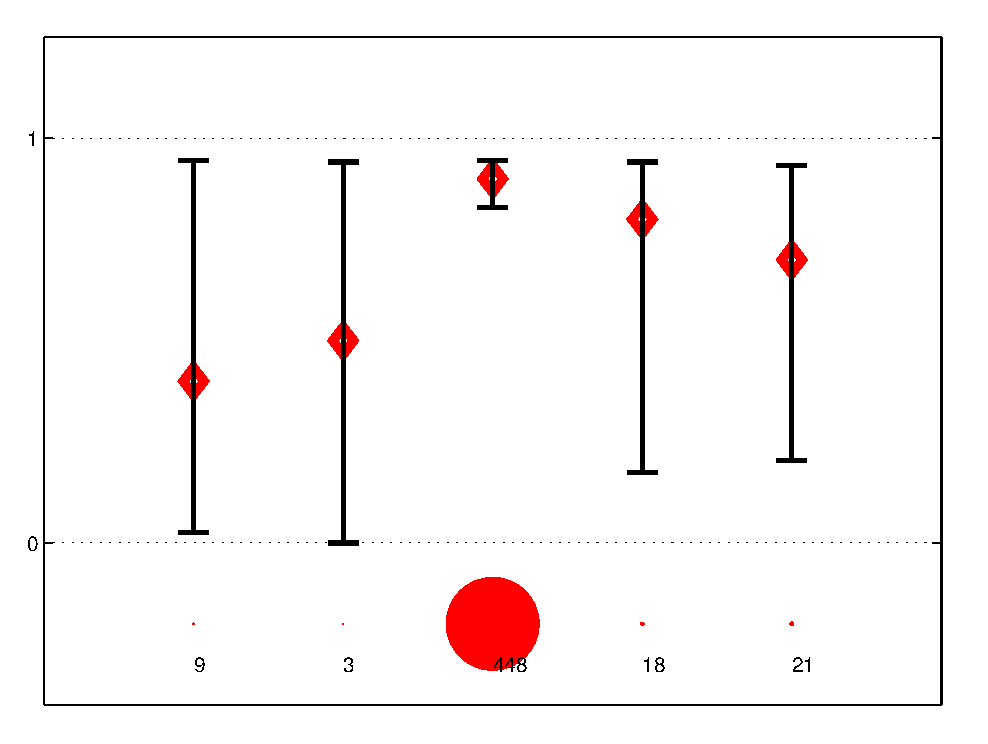
\includegraphics[width=0.95\linewidth]{KLUCBillustration}
        \end{minipage}
        \begin{minipage}{0.4\linewidth}
            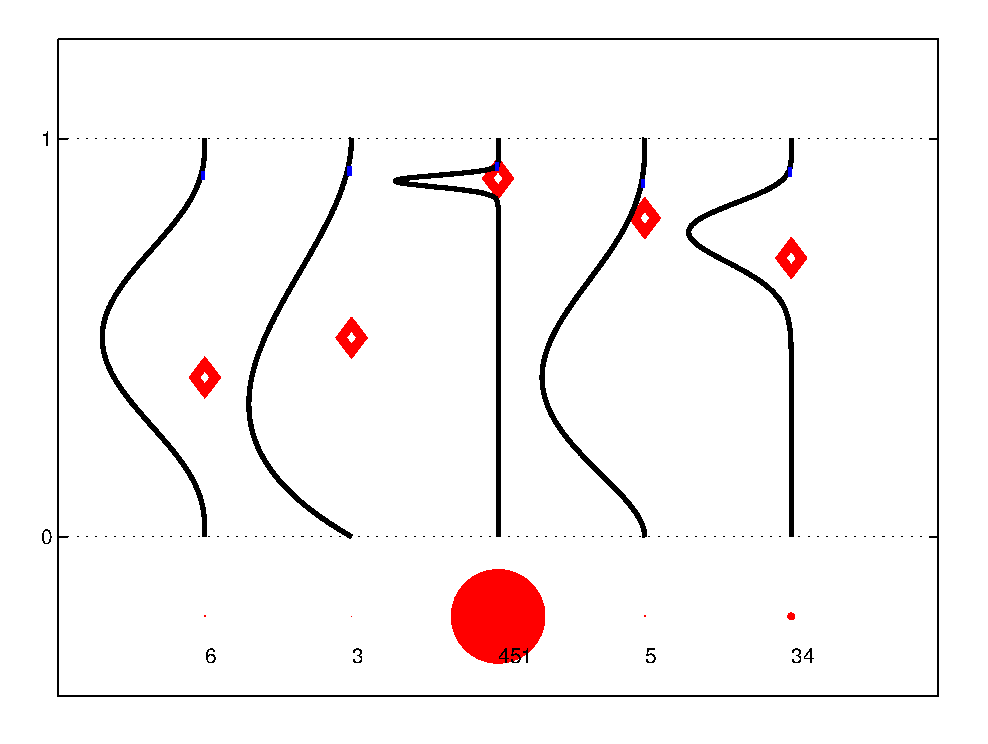
\includegraphics[width=0.95\linewidth]{BayesUCB}
        \end{minipage}
    \end{center}

\end{frameO}



\begin{frameO}[Example: Bernoulli bandits]

    \vspace{0.3cm}

    Bernoulli bandit model $\bm \mu = (\mu_1,\dots,\mu_K)$

    \begin{itemize}
        \item \textbf{Bayesian view}: $\mu_1,\dots,\mu_K$ are \blue random variables \black

              \vspace{-0.4cm}

              \[\blue\text{prior distribution}\black: \ \ \ \mu_a \sim \cU([0,1]) \ \ \ \]

              \vspace{-0.5cm}

        \item[\ding{220}] \underline{posterior distribution}:
              \vspace{-0.6cm}

              \begin{eqnarray*} \pi_a(t) &=& \cL\left(\mu_a | R_1,\dots,R_t \right)\\
                  & = & \red \mathrm{Beta}\Big(\underbrace{S_a(t)}_{\# ones} +1, \underbrace{N_a(t) - S_a(t)}_{\# zeros} +1\Big)
              \end{eqnarray*}
    \end{itemize}

    \vspace{-0.9cm}

    \begin{center}
        \begin{minipage}{0.35\linewidth}
            \centering
            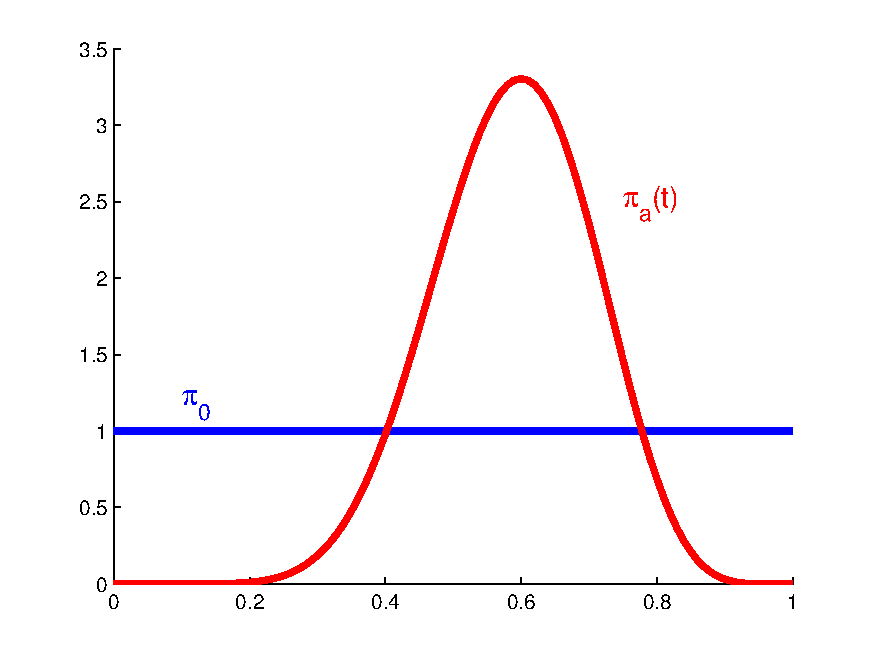
\includegraphics[width=\linewidth]{BayesianStuff}
        \end{minipage}
        \begin{minipage}{0.35\linewidth}
            \centering
            \includegraphics[width=\linewidth]{BayesianStuff2}
        \end{minipage}
    \end{center}

    \vspace{-0.5cm}

    $S_a(t) = \sum_{s=1}^t R_s \ind_{(A_s = a)}$ sum of the rewards from arm $a$

\end{frameO}


\begin{frameO}[Bayesian algorithm]

    \vspace{0.3cm}

    A \blue Bayesian bandit algorithm \black exploits the posterior distributions of the means to decide which arm to select.

    \begin{center}
        \includegraphics[width=0.7\textwidth]{BayesCNRS}
    \end{center}


\end{frameO}



\subsection{Solving the Bayesian MAB}

\begin{frame}[c]
    \begin{changemargin}{-0.5cm}{-0.5cm}
        \begin{center}
            \vspace{-0.3in}
            \textbf{\huge Bayesian Bandits}
            \vspace{1.5cm}

            \textbf{\Large Insights from the Optimal Solution}	\\[0.5cm]
            \textcolor{darkgray}{\textbf{\Large Bayes-UCB}\\[0.5cm]		}
            \textcolor{darkgray}{	\textbf{\Large Thompson Sampling}	\\[0.5cm]			}
        \end{center}
    \end{changemargin}
\end{frame}


\begin{frameO}[Some insights from the Bayesian solution]

    \vspace{0.5cm}

    Bandit model $(\cB(\mu_1),\dots,\cB(\mu_K))$
    \[\pi_a^t = \mathrm{Beta}\Big(\underbrace{S_a(t)}_{\# ones} +1, \underbrace{N_a(t) - S_a(t)}_{\# zeros} +1\Big)\]
    The posterior distribution is fully summarized by \blue a matrix containing the number of ones and zeros observed \black for each arm.


    \begin{center}
        \begin{minipage}{0.4\textwidth}
            \[\Pi^t =
                \begin{pmatrix}
                    0  & 2 \\
                    3  & 3 \\
                    13 & 4 \\
                    5  & 2 \\
                    1  & 3 \\
                \end{pmatrix}
            \]

        \end{minipage}
        \begin{minipage}{0.5\textwidth}
            \includegraphics[width=0.8\linewidth]{posterior.jpg}
        \end{minipage}
    \end{center}

    \vspace{-0.4cm}

    \begin{center}
        \red ``State'' $\Pi^t$ \black  that evolves.
    \end{center}

\end{frameO}



\begin{frameO}[A first Markov Decision Process]

    \vspace{0.3cm}

    After each arm selection $A_t$, we receive a reward $R_t$ such that
    \[\bP\left(R_t = 1 | \Pi^{t-1} = \Pi , A_t = a\right) = \underbrace{\frac{\Pi^t(a,1)+1}{\Pi^t(a,1)+ \Pi^t(a,2)+2}}_{\text{mean of } \pi_a(t-1)}\]
    and the posterior gets updated:
    \begin{eqnarray*}
        \Pi^t(A_t, 1) &=& \Pi^{t-1}(A_t, 1) + R_t\\
        \Pi^t(A_t, 2) &=& \Pi^{t-1}(A_t, 2) + (1-R_t)
    \end{eqnarray*}

    \textbf{Example of transition:}

    \alt<2>{\[
            \begin{pmatrix}
                1      & 2      \\
                \red 5 & \red 1 \\
                0      & 2      \\
            \end{pmatrix}
            \overset{\red A_t=2}{\longrightarrow}
            \begin{pmatrix}
                1      & 2      \\
                \red 5 & \red 2 \\
                0      & 2      \\
            \end{pmatrix}
            \textit{if} \ R_{t}=0
        \]}{\[
            \begin{pmatrix}
                1      & 2      \\
                \red 5 & \red 1 \\
                0      & 2      \\
            \end{pmatrix}
            \overset{\red A_t=2}{\longrightarrow}
            \begin{pmatrix}
                1      & 2      \\
                \red 6 & \red 1 \\
                0      & 2      \\
            \end{pmatrix}
            \textit{if} \ R_{t}=1
        \]
    }

    \hfill  $\rightarrow $ \blue Markov Decision Process with state $\Pi^t$

\end{frameO}


\begin{frameO}[An exact solution]

    Solving the Bayesian bandit $\leftrightarrow$ \blue maximizing rewards in some Markov Decision Process \black (modern perspective)

    \vspace{0.3cm}

    There exists an exact solution to

    \vspace{0.5cm}

    \begin{minipage}{0.45\linewidth}
        \begin{itemize}
            \item The finite-horizon MAB:
        \end{itemize}
        \[\red \argmax_{(A_t)} \ \bE_{\bm{\mu} \sim \pi}\left[\sum_{t=1}^T R_t\right]\black\]
    \end{minipage}
    \begin{minipage}{0.54\linewidth}
        \begin{itemize}
            \item The discounted MAB:
        \end{itemize}
        \[\red \argmax_{(A_t)} \ \bE_{\bm{\mu} \sim \pi}\left[\sum_{t=1}^\infty \gamma^{t-1} R_t\right]\black\]
    \end{minipage}

    \begin{center}
        \gray[Berry and Fristedt, \textit{Bandit Problems}, 1985]
    \end{center}


    \textbf{Optimal solution}: solution to \blue dynamic programming equations\black.

    \vspace{0.2cm}

    \textbf{Problem:} The state space is very large

    \vspace{0.2cm}

    \hfill $\rightsquigarrow$ \red often intractable



\end{frameO}




\begin{frameO}[Gittins indices]

    \vspace{0.4cm}

    \color{gray}[Gittins 79]\color{black}: the solution of the \blue discounted\black \ MAB
    \[\argmax_{(A_t)} \ \bE_{\bm{\mu} \sim \pi}\left[\sum_{t=1}^\infty \gamma^{t-1} R_t\right]\black\]
    is an \textbf{index policy}:
    \[A_{t+1} = \underset{a=1 \dots K}{\text{argmax}} \ \red G_\gamma(\pi_a(t))\black.\]

    \begin{itemize}
        \item \textbf{The Gittins indices}:
    \end{itemize}

    \begin{orangeblock}{}
        \[G_\gamma(p) = \inf \{ \lambda \in \R : V_\gamma^*(p,\lambda)  = 0\},\]
        with
        \[V^*_\gamma(p,\lambda) = \sup_{\substack{\text{stopping } \\ \text{times} \ \red \tau > 0\black}} \ \bE_{\substack{Y_t \overset{\text{i.i.d}}{\sim} \cB(\mu) \\ \mu \sim p}}\left[\sum_{t=1}^\tau \gamma^{t-1}(Y_t- \lambda)\right].\]
    \end{orangeblock}

    \begin{center} \blue
        ``price worth paying for committing to arm $\mu\sim p$

        when rewards are discounted by $\alpha$''
    \end{center}
\end{frameO}


\begin{frameO}[Gittins indices for Finite Horizon?]


    \vspace{0.5cm}

    The solution of the \blue finite horizon \black \ MAB
    \[\argmax_{(A_t)} \ \bE_{\bm{\mu} \sim \pi}\left[\sum_{t=1}^T R_t\right]\black\]
    is NOT an index policy. \color{gray} [Berry and Fristedt 85]\color{black}

    \begin{itemize}
        \item \textbf{Finite-Horizon Gittins indices}:

              depend on the \red remaining time to play r \black
    \end{itemize}

    \begin{orangeblock}{}
        \[G(p,r) = \inf \{ \lambda \in \R : V_r^*(p,\lambda)  = 0\},\]
        with
        \[V^*_r(p,\lambda) = \sup_{\substack{\text{stopping times} \\ \red 0< \tau \leq r\black}} \ \bE_{\substack{Y_t \overset{\text{i.i.d}}{\sim} \cB(\mu) \\ \mu \sim p}}\left[\sum_{t=1}^\tau (Y_t- \lambda)\right].\]
    \end{orangeblock}

    \begin{center}\blue
        ``price worth paying for playing arm $\mu\sim p$ for at most $r$ rounds''
    \end{center}

\end{frameO}

\begin{frameO}[Finite-Horizon Gittins algorithm]

    \vspace{0.3cm}

    \textbf{FH Gittins algorithm:}
    \[A_{t+1} = \argmax_{a=1 \dots K} \ \red G(\pi_a(t-1),T-t)\black\]
    does NOT coincide with the Bayesian optimal solution but is conjectured to be a good approximation!

    \vspace{-0.4cm}

    \begin{center}
        \includegraphics[height=0.4\textheight]{DPGitt}
    \end{center}

    \vspace{-0.5cm}

    \begin{itemize}
        \item good performance in terms of frequentist regret as well
        \item ... with logarithmic regret \color{gray} [Lattimore, 2016]
    \end{itemize}


\end{frameO}


\begin{frameO}[Approximating the FH-Gittins indices]

    \begin{itemize}
        \item \color{gray} [Burnetas and Katehakis, 03]\black : when $n$ is large,
    \end{itemize}
    \[G(\pi_a(t-1),n) \simeq \max \left\{ q :  N_a(t)\times \kl\left(\hat{\mu}_a(t),q\right) \leq \ln \left(\color{red}\frac{n}{N_a(t)}\color{black}\right)\right\}\]

    \vspace{0.5cm}

    \begin{itemize}
        \item \color{gray} [Lai, 87]\black : the index policy associated to
    \end{itemize}
    \[I_a(t)=\max \left\{ q : N_a(t) \times \kl\left(\hat{\mu}_a(t),q\right) \leq \ln\left(\color{red}\frac{T}{N_a(t)}\color{black}\right)\right\}\]
    \begin{itemize}
        \item[] is a good approximation of the Bayesian solution for large $T$.
    \end{itemize}

    \vspace{0.3cm}

    \begin{itemize}
        \item[\ding{220}] looks like the \blue \klUCB{} index\black, with a \blue different exploration rate\black...
    \end{itemize}


\end{frameO}


\begin{frame}[c]
    \begin{changemargin}{-0.5cm}{-0.5cm}
        \begin{center}
            \vspace{-0.3in}
            \textbf{\huge Bayesian Bandits}
            \vspace{1.5cm}

            \textcolor{darkgray}{\Large \textbf{Insights from the Optimal Solution}}	\\[0.5cm]
            \textbf{{\Large Bayes-UCB}\\[0.5cm]		}
            \textcolor{darkgray}{	\textbf{\Large Thompson Sampling}	\\[0.5cm]			}
        \end{center}
    \end{changemargin}
\end{frame}


\subsection{Bayes-UCB}

\begin{frameO}[The Bayes-UCB algorithm]

    \vspace{0.3cm}

    \begin{itemize}
        \item $\Pi_0=(\pi_1(0),\dots,\pi_K(0))$ be a prior distribution over $(\mu_1,...,\mu_K)$
        \item $\Pi_t=(\pi_1(t),\dots, \pi_K(t))$ be the posterior distribution over the means $(\mu_1,...,\mu_K)$ after $t$ observations
    \end{itemize}

    \begin{orangeblock}{}
        The \textbf{Bayes-UCB algorithm} chooses at time $t$
        $$
            \color{red}A_{t+1} = \argmax_{a = 1,\dots,K} \  Q\left(1-\frac{1}{t(\ln t )^c}, \pi_a(t)\right) \color{black}
        $$
        where $Q(\alpha,\pi)$ is the quantile of order $\alpha$ of the distribution $\pi$.
    \end{orangeblock}

    \vspace{0.3cm}

    \alt<3>{\color{blue} Gaussian rewards with Gaussian prior:\color{black}
        %\vspace{0.2cm}
        \begin{itemize}
            \item $\pi_{a}(0) \overset{i.i.d}{\sim} \mathcal{N}(0,\kappa^2)$ \\
            \item $\pi_a(t) = \mathcal{N}\left(\frac{S_a(t)}{N_a(t) + {\sigma^2}/\kappa^2},\frac{\sigma^2}{N_a(t) + {\sigma^2}/\kappa^2}\right)$
        \end{itemize}}{
        \alt<2>{
            \color{blue} Bernoulli reward with uniform prior:\color{black}
            %\vspace{0.2cm}
            \begin{itemize}
                \item $\pi_{a}(0) \overset{i.i.d}{\sim} \mathcal{U}([0,1])=\text{Beta}(1,1)$ \\
                \item $\pi_a(t) = \text{Beta}(S_{a}(t)+1,N_{a}(t) - S_{a}(t) +1)$
            \end{itemize}}{\vspace{-1cm}
            \begin{center}
                \includegraphics[height=4.5cm,angle=-90]{beta_quantile}
            \end{center}

        }}


\end{frameO}

\begin{frameO}[Bayes UCB in action]

    \begin{center}
        \movie{\includegraphics[width=0.9\textwidth]{tryBayesUCB.pdf}}{tryBayesUCB.avi}
    \end{center}



\end{frameO}

\begin{frameO}[Theoretical results in the Bernoulli case]
    \vspace{0.3cm}

    \begin{itemize}
        \item \textbf{Bayes-UCB is \textcolor{red}{asymptotically optimal} for Bernoulli rewards}
    \end{itemize}

    \vspace{0.3cm}

    \begin{orangeblock}{Theorem \color{gray}[K.,Capp\'e,Garivier 2012]}

        Let $\varepsilon > 0$. The Bayes-UCB algorithm using a uniform prior over the arms and parameter $c  \geq 5$ satisfies
        \vspace{-0.3cm}
        \[\mathbb{E}_{\bm\mu}[N_a(T)]\leq \frac{1+\varepsilon}{\kl(\mu_a,\mu_\star)}\ln(T) + o_{\varepsilon,c}\left(\ln(T)\right).\]
        %\begin{align*}
        % &  \bE[N_a(T)] \leq \frac{1+\varepsilon}{d(\mu_a,\mu_1)}\ln(T) +
        % \sqrt{\ln T + 5\ln\ln T} \sqrt{\frac{2\pi(1+\varepsilon)^3d'(\mu_a,\mu_1)^2}{d(\mu_a,\mu_1)^3}} \\
        %& \ \ \ \ \ \ \ \ \ + \left(\frac{1+\varepsilon}{d(\mu_a,\mu_1)} +
        %\frac{2e+3}{1-\mu_1}\right)\ln \ln T + 27 +  2(1+\varepsilon)^2 \left(\frac{d'(\mu_a,\mu_1)}{d(\mu_a,\mu_1)}\right)^2.
        %\end{align*}
    \end{orangeblock}

\end{frameO}


\begin{frameO}[Links with \klUCB]

    \begin{alertblock}{Lemma \gray [K. et al., 12]}
        The index $q_a(t)$ used by Bayes-UCB satisfies \[\red\tilde{u}_a(t) \leq q_a(t) \leq u_a(t)\]

        \vspace{-0.7cm}

        where
        \begin{eqnarray*}
            u_a(t)\! & = &\!\! \max \left\{ q  : \kl \left(\frac{S_a(t)}{N_a(t)},q\right) \leq \frac{\ln(t) +c\ln(\ln(t))}{N_a(t)}\right\} \\
            \tilde{u}_a(t) \!& = &\!\! \max\left\{ q : \kl\left(\frac{S_a(t)}{N_a(t)+1},q\right) \leq \frac{\ln\left(\color{red}\frac{t}{N_a(t)+2}\color{black}\right) + c\ln(\ln(t))}{(N_a(t)+1)}\right\}
        \end{eqnarray*}
    \end{alertblock}

    \textbf{Proof}: rely on the \blue Beta-Binomial trick \black:
    \[F_{\text{Beta}(a,b)}(x) = 1 - F_{\text{Bin}(a+b - a , x)}(a-1)\]

    \hfill\gray [Agrawal and Goyal, 12]
\end{frameO}

\begin{frameO}[Beyond Bernoulli bandits]

    \begin{itemize}
        \item For \red one-dimensional exponential families \black, Bayes-UCB rewrites
              \[
                  A_{t+1} = \underset{a}{\text{argmax}} \  Q\left(1-\frac{1}{t(\ln t )^c}, \pi_{a,N_a(t),\hat{\mu}_a(t)}\right)
              \]
    \end{itemize}

    \textbf{Extra assumption:} there exists $\mu^-,\mu^+$ such that for all $a$,
    $ \blue\mu_a \in [\mu^-, \mu^+]\black$


    \begin{orangeblock}{Theorem \gray [K. 17]}
        Let $\overline{\mu}_a(t) = (\hat{\mu}_a(t) \vee \mu^-)\wedge \mu^+$. The index policy

        \vspace{-0.3cm}

        \[
            A_{t+1} = \underset{a}{\text{argmax}} \   Q\left(1-\frac{1}{t(\ln t )^c}, \pi_{a,N_a(t),\blue\overline{\mu}_a(t)\black}\right)
        \]

        with parameter $c\geq 7$ is such that, for all $\varepsilon>0$,

        \vspace{-0.3cm}

        \[\red\bE_{\bm \mu}[N_a(T)] \leq \frac{1+\varepsilon}{\kl(\mu_a,\mu_\star)}\ln(T) + O_{\varepsilon}(\sqrt{\ln(T)})\black.\]

        \vspace{-0.3cm}

    \end{orangeblock}


\end{frameO}

\begin{frameO}[An interesting by-product]

    \vspace{0.3cm}

    \begin{itemize}
        \item Tools from the analysis of Bayes-UCB can be used to analyze two variants of \klUCB{}
    \end{itemize}

    \begin{orangeblock}{\klUCB-H$^+$}
        \[u_a^{H,+}(t)=\max\left\{q :  N_a(t)\times \kl\left(\hat{\mu}_a(t),q\right) \leq \ln\left(\blue\frac{T\ln^c T}{N_a(t)}\black\right)\right\}\]
    \end{orangeblock}

    \begin{orangeblock}{\klUCB$^+$}
        \[u_a^{+}(t)=\max\left\{q  :  N_a(t) \times \kl\left(\hat{\mu}_a(t),q\right) \leq \ln\left(\blue\frac{t\ln^c t}{N_a(t)}\black\right)\right\}\]
    \end{orangeblock}

    \vspace{0.2cm}

    The index policy associated to $u_a^{H,+}(t)$ and $u_a^{+}(t)$ satisfy, for all $\varepsilon>0$,
    \[\red\bE_{\bm\mu}[N_a(T)] \leq \frac{1+\varepsilon}{\kl(\mu_a,\mu_\star)}\ln(T) + O_{\varepsilon}(\sqrt{\ln(T)})\black.\]



\end{frameO}

\begin{frame}[c]
    \begin{changemargin}{-0.5cm}{-0.5cm}
        \begin{center}
            \vspace{-0.3in}
            \textbf{\huge Bayesian Bandits}
            \vspace{1.5cm}

            \textcolor{darkgray}{\Large \textbf{Insights from the Optimal Solution}}	\\[0.5cm]
            \textcolor{darkgray}{\textbf{{\Large Bayes-UCB}\\[0.5cm]		}}
            \textcolor{black}{	\textbf{\Large Thompson Sampling}	\\[0.5cm]			}
        \end{center}
    \end{changemargin}
\end{frame}



\subsection{Thompson Sampling}

\begin{frameO}[Historical perspective]
    {\small
        \begin{itemize}
            \item[1933] Thompson: in the context of clinical trial, the allocation of a treatment should be some increasing function of its \red posterior probability to be optimal \black
            \item[2010] Thompson Sampling rediscovered under different names

                  Bayesian Learning Automaton \gray [Granmo, 2010] \black

                  Randomized probability matching \gray [Scott, 2010]\black
            \item[2011] An empirical evaluation of Thompson Sampling: \red an efficient algorithm\black, beyond simple bandit models

                  \gray [Li and Chapelle, 2011]\black

            \item[2012] First (logarithmic) \red regret bound \black for Thompson Sampling

                  \gray [Agrawal and Goyal, 2012]\black

            \item[2012] Thompson Sampling is \red asymptotically optimal for Bernoulli bandits \black


                  \gray [K., Korda and Munos, 2012][Agrawal and Goyal, 2013]\black


            \item[2013-] Many \red successful uses of Thompson Sampling \black beyond Bernoulli bandits (contextual bandits, reinforcement learning)



        \end{itemize}}

\end{frameO}

\begin{frameO}[Thompson Sampling]

    \vspace{0.4cm}

    \textbf{Two equivalent interpretations}:
    \begin{itemize}\item
              \small ``select an arm at random according to its probability of being the best''
        \item ``draw a possible bandit model from the posterior distribution and act optimally in this sampled model''
    \end{itemize}

    \vspace{-0.4cm}

    \hfill \red $\neq$ optimistic \black

    \begin{orangeblock}{Thompson Sampling: a randomized Bayesian algorithm}
        \[
            \left\{
            \begin{array}{l}
                \forall a\in\{1..K\}, \ \  \theta_{a}(t) \sim \pi_{a}(t) \\
                A_{t+1}  =  \underset{a = 1 \dots K}{\text{argmax}} \ \theta_{a}(t).
            \end{array}
            \right.
        \]
    \end{orangeblock}

    \vspace{-0.2cm}

    \begin{center}
        \includegraphics[height=1.5cm]{TS1}
        \includegraphics[height=1.5cm]{TS2}
    \end{center}


\end{frameO}


\begin{frameO}[Thompson Sampling is asymptotically optimal]

    \vspace{0.3cm}

    \begin{orangeblock}{Problem-dependent regret}
        \[\forall \varepsilon>0, \ \ \bE_{\bm\mu}[N_a(T)] \leq (\color{red}1+\varepsilon\color{black})\frac{1}{\color{red}\kl(\mu_a,\mu_\star)\color{black}}\ln(T) + o_{\mu,\varepsilon}(\ln(T)).\]

        \vspace{-0.3cm}
    \end{orangeblock}


    This results holds:
    \begin{itemize}
        \item for \red Bernoulli bandits\black, with a \blue uniform prior

              \gray [K. Korda, Munos 12][Agrawal and Goyal 13] \black
        \item for \red Gaussian bandits\black, with \blue Gaussian prior\black \gray [Agrawal and Goyal 17]\black
        \item for \red exponential family bandits\black, with \blue Jeffrey's prior \gray [Korda et al. 13]\black
    \end{itemize}

    \begin{orangeblock}{Problem-independent regret \gray[Agrawal and Goyal 13]}
        For Bernoulli and Gaussian bandits, Thompson Sampling satisfies

        \vspace{-0.3cm}

        \[\cR_{\bm\mu}(\texttt{TS},T) =O \left(\sqrt{KT\ln(T)}\right).\]

        \vspace{-0.4cm}

    \end{orangeblock}

    \vspace{-0.2cm}

    \begin{itemize}
        \item Thompson Sampling is also \red asymptotically optimal for Gaussian with unknown mean and variance \black \gray [Honda and Takemura, 14]
    \end{itemize}


\end{frameO}




\begin{frameO}[Understanding Thompson Sampling]

    \vspace{0.3cm}

    \begin{itemize}
        \item a key ingredient in the analysis of \gray [K. Korda and Munos 12] \black
    \end{itemize}

    \begin{orangeblock}{Proposition}
        There exists constants $b = b(\mu)\in (0,1)$ and $C_b<\infty$ such that

        \vspace{-0.4cm}

        $$
            \sum_{t = 1}^{\infty} \bP\left(N_1(t)\leq t^b\right)\leq C_b.
        $$
    \end{orangeblock}

    \vspace{-0.5cm}

    \[
        \left\{N_1(t) \leq  t^b\right\}=  \{  \text{there exists a time range of length at least} \ t^{1-b}-1 \]

    \vspace{-0.3cm}

    \hspace{3.5cm} with no draw of arm 1 $\}$


    \vspace{-0.3cm}

    \begin{center}
        \includegraphics[height=4cm]{thompson}
    \end{center}

\end{frameO}



\begin{frameO}[Bayesian versus Frequentist algorithms]

    \begin{itemize}
        \item \blue Short horizon\black, $T=1000$ (average over $N=10000$ runs)
    \end{itemize}

    \begin{center}
        \includegraphics[width=0.6\textwidth]{GittinsFreq02025}

        $\mu_1 = 0.2, \mu_2=0.25$
    \end{center}

\end{frameO}

\begin{frameO}[Bayesian versus Frequentist algorithms]

    \begin{itemize}
        \item \blue Long horizon\black, $T=20000$ (average over $N=50000$ runs)
    \end{itemize}

    \begin{center}
        \includegraphics[width=\textwidth]{Curves.png}

        \vspace{0.2cm}

        10 arms bandit problem $\mu=[0.1 \ 0.05 \ 0.05 \ 0.05 \ 0.02 \ 0.02 \ 0.02 \ 0.01 \ 0.01 \ 0.01]$
    \end{center}

\end{frameO}




\begin{frameTI}
    \begin{center}
        \color{white} \Huge \textsc{Other randomized}

        \textsc{algorithms}
    \end{center}
    \vspace*{-4pt}
\end{frameTI}

\begin{frameO}[Limitation of existing approaches]

    \begin{orangeblock}{Two families of asymptotically optimal algorithms}
        \begin{itemize}
            \item Confidence bound algorithms

            \item Thompson Sampling
        \end{itemize}
    \end{orangeblock}

    \begin{itemize}
        \item Provably optimal finite-time regret under the assumption that the rewards distribution belong to \blue some class $\cD$\black
        \item A \rcol{different algorithm for each $\cD$}: TS or \klUCB{} for Bernoulli, Poisson, for Exponential, etc.
    \end{itemize}

    \begin{center}
        Can we build a \red universal algorithm \black that would be asymptotically optimal over different classes $\cD$?
    \end{center}
\end{frameO}


\begin{frameO}[A Puzzling strategy]

    \begin{center}
        \large{\HL{B}est  \HL{E}mpirical \HL{S}ub-sampling \HL{A}verage}

        \vspace{0.2cm}

        \textcolor{gray}{"Sub-sampling for multi-armed bandits",\\ Baransi, Maillard, Mannor \textit{ECML}, 2014.}
    \end{center}

    \begin{orangeblock}{BESA}
        \begin{itemize}
            \item Competitive regret against state-of-the-art for various $\cD$.
            \item Same algorithm for all $\cD$.
            \item Not relying on upper confidence bounds, not Bayesian...
            \item ...and extremely simple to implement.
        \end{itemize}
    \end{orangeblock}


    \begin{itemize}
        \item[\ding{220}] How? Optimality? For which distributions ?
    \end{itemize}



\end{frameO}



\begin{frameO}[Going back to "Follow the leader"]
    {\bf FTL}
    \begin{enumerate}
        \item Play each arm once.
        \item At time $t$, define $\tilde \mu_{a}(t) = \hat \mu(R_{1:N_{a}(t)}^a)$ for all $a\in\cA$.
              \begin{itemize}
                  \item $\hat \mu(\cX)$: empirical average of population $\cX$.
                  \item $R_{1:N_{a}(t)}^a = \{ R_s : A_s=a, s \leq t\}$
              \end{itemize}
        \item Choose (break ties in favor of the smallest $N_a(t)$)
              \[
                  A_{t+1} = \argmax_{a'\in\{a,b\}} \tilde \mu_{a'}(t)\,.
              \]
    \end{enumerate}

    \begin{orangeblock}{Properties}
        \begin{itemize}
            \item Generally bad: linear regret.
            \item A variant ($\varepsilon$\texttt{-greedy}) performs ok if well-tuned \gray[Auer et al, 2002]\black.
        \end{itemize}
    \end{orangeblock}

    \vspace{-5mm}
\end{frameO}


\begin{frameO}[Follow the FAIR leader (aka BESA)]

    \textbf{Idea:} Compare two arms based on "equal opportunity"

    i.e. same number of observations.

    \vspace{0.3cm}

    \begin{orangeblock}{}
        {\bf BESA} at time $t$ for two arms $a,b$:

        \begin{enumerate}
            \item Sample two sets of indices $\cI_a(t)\sim {\texttt{Wr}}(N_{a}(t);N_{b}(t))$ and $\cI_b(t)\sim {\texttt{Wr}}(N_{b}(t);N_{a}(t))$.
                  \begin{itemize}
                      \item ${\texttt{Wr}}(n,N)$: sample $n$ points from $\{1,\dots,N\}$ without replacement (return all the set if $n\geq N$).
                  \end{itemize}
            \item Define $\tilde \mu_{a}(t) = \hat \mu(R_{1:N_{a}(t)}^a(\cI_a(t)))$ and $\tilde \mu_{b}(t) = \hat \mu(R_{1:N_{t,b}}^b(\cI_b(t)))$.
            \item Choose (break ties in favor of the smallest $N_{a'}(t)$)
                  \[A_{t+1} = \argmax_{a'\in\{a,b\}} \tilde \mu_{a'}(t)\,.\]
        \end{enumerate}
    \end{orangeblock}

    \begin{itemize}
        \item more than two arms? tournament.
    \end{itemize}

\end{frameO}


\begin{frameO}[Example]

    \begin{itemize}
        \item $\cX=(x_1,\dots,x_N)$,a finite population of $N$ real points.

              \begin{tabular}{|c|c|c|c|c|c|c|c|c|}
                  \hline
                  $x_1$ & $x_2$ & $x_3$ & $x_4$ & $x_5$ & \dots & $x_{N-2}$ & $x_{N-1}$ & $x_N$ \\
                  \hline
              \end{tabular}

              \bigskip
        \item Sub-sample of size $n\leq N$ from $\cX$: $X_1,\dots,X_n$ picked uniformly randomly without replacement from $\cX$.

              \begin{tabular}{|c|c|c|c|c|c|c|c|c|}
                  \hline
                  $
                  x_1$ & \cellcolor{blue!25}$X_{n-1}$ & \cellcolor{blue!25}$X_1$ & $x_4$ & \cellcolor{blue!25}$X_2$ & \dots & $x_{N-2}$ & \cellcolor{blue!25}$X_{n}$ & $x_N$ \\
                  \hline
              \end{tabular}


              \bigskip

        \item	Example: $N_{a}(t)=3$ and $N_{b}(t)=10$:

              $\cI_{a}(t) = \{1,2,3\}$,

              $|\cI_{b}(t)|=3$, sampled without replacement from $\{1,\dots,10\}$.
    \end{itemize}

\end{frameO}


\begin{frameO}[Good practical performance ($T = 20,000$, $N=50,000$)]

    \vspace{0.2cm}

    \begin{itemize}
        \item 10 {\bf Bernoulli}$(0.1, 3\{0.05\}, 3\{0.02\}, 3\{0.01\})$
    \end{itemize}

    \begin{center}
        \begin{tabular}{|c|ccccc|}
            \hline
                      & \HL{BESA}  & kl-UCB & kl-UCB+    & TS    & Others  \\
            \hline
            Regret    & {\bf 74.4} & 121.2  & {\bf 72.8} & 83.4  & 100-400 \\
            Beat BESA & -          & 1.6\%  & 35.4\%     & 3.1\% &         \\
            Run Rime  & 13.9X      & 2.8X   & 3.1X       & X     &         \\
            \hline
        \end{tabular}

        \vspace{0.3cm}

        \includegraphics[width=\textwidth]{BESA1}

    \end{center}

    \vspace{-0.4cm}

    Others: UCB, Moss, UCB-Tunes, DMED, UCB-V.

    \vspace{-0.3cm}

    \flushright{\footnotesize{(Credit: Akram Baransi)}}

\end{frameO}


\begin{frameO}[Good practical performance ($T = 20,000$, $N=50,000$)]

    \vspace{0.3cm}

    \begin{itemize}
        \item {\bf Exponential}$(\frac{1}{5},\frac{1}{4},\frac{1}{3},\frac{1}{2},1)$
    \end{itemize}

    \vspace{-0.5cm}

    \begin{center}
        \begin{tabular}{|c|ccccc|}
            \hline
                      & \HL{BESA} & KL-UCB-exp & UCB-tuned & FTL 10 & Others      \\
            \hline
            Regret    & {\bf	53.3} & 65.7       & 97.6      & 306.5  & 60-110,120+ \\
            Beat BESA & -         & 5.7\%      & 4.3\%     & -      &             \\
            Run Rime  & 6X        & 2.8X       & X         & -      &             \\
            \hline
        \end{tabular}

        \vspace{0.3cm}

        \includegraphics[width=\textwidth]{BESA2}
    \end{center}

    \vspace{-0.3cm}

    Others: UCB, Moss, kl-UCB,UCB-V.

    \vspace{-5mm}
    \flushright{\footnotesize{(Credit: Akram Baransi)}}
\end{frameO}


\begin{frameO}[Good practical performance ($T = 20,000$, $N=50,000$)]

    \vspace{0.2cm}

    \begin{itemize}
        \item {\bf Poisson}$(\{\frac{1}{2}+\frac{i}{3}\}_{i=1,\dots,6})$
    \end{itemize}

    \begin{center}
        %\hspace{-1cm}
        \begin{tabular}{|c|cccc|}
            \hline
                      & \HL{BESA} & KL-UCB-Poisson & kl-UCB & FTL 10 \\
            \hline
            Regret    & \bf{19.4} & 25.1           & 150.6  & 144.6  \\
            Beat BESA & -         & 4.1\%          & 0.7\%  & -      \\
            Run Rime  & 3.5X      & 1.2X           & X      & -      \\
            \hline
        \end{tabular}

        \vspace{0.3cm}

        \includegraphics[width=\textwidth]{BESA3}
    \end{center}



    \vspace{-5mm}
    \flushright{\footnotesize{(Credit: Akram Baransi)}}

    \vspace{-8mm}
\end{frameO}



\begin{frameO}[Regret bound  (slightly simplified statement)]

    With two arms $\{\star,a\}$, define

    \vspace{-0.5cm}

    \[
        \alpha(M,n) =\bE_{Z^\star\sim \nu_{\star,n}}\Bigg[ \bigg(\bP_{Z\sim\nu_{a,n}}(Z>Z^\star)
            + {\color{gray}\frac{1}{2}\bP_{Z\sim\nu_{a,n}}(Z=Z^\star)}\bigg)^M\Bigg]\,.
    \]

    \vspace{-5mm}

    \begin{orangeblock}{Theorem \gray[Baransi et al. 14]}
        If $\exists \alpha \in(0,1), c>0$ such that $\alpha(M,1) \leq c\alpha^M$, then
        \[
            \cR_{\nu}(\texttt{BESA},T) \leq \frac{11\ln(T)}{\mu_\star-\mu_a} + C_{\nu} + O(1)\,.
        \]
    \end{orangeblock}
    %

    \begin{redblock}{Example}
        \begin{itemize}
            \item Bernoulli $\mu_a,\mu_\star$: $\alpha(M,1) =O\Big(\big(\frac{\mu_a  \vee (1-\mu_a)}{2}\big)^M\Big)$
        \end{itemize}
    \end{redblock}

    \textbf{Future work:} understand when BESA fails, and whether it can be asymptotically optimal in some cases...
\end{frameO}



\begin{frameO}[Adversarial bandits]

    Another class of (randomized) bandit algorithms that do not exploit any assumption on $\cD$ is that of \red adversarial bandit algorithms\black.

    \begin{center}\gray [Auer, Cesa-Bianchi, Freund, Shapire,

            \textit{The non-stochastic multi-armed bandit}, 2002]
    \end{center}

    \vspace{0.3cm}

    \begin{center}
        {\Large Can we achieve $O(\sqrt{KT})$ regret with respect to the best static action if the rewards are arbitrarily generated?}
    \end{center}


    \vspace{0.4cm}

    \hfill Some answers in the next classes and practical sessions!
\end{frameO}


\begin{frameTI}
    \begin{center}
        {\textcolor{white} {\Huge \textsc{Summary} }}
    \end{center}
    \vspace*{-4pt}
\end{frameTI}

\begin{frameO}[Take-home messages]

    Now you are aware of:
    \begin{itemize}
        \item several methods for facing an exploration/exploitation dilemma
        \item notably two powerful classes of methods
              \begin{itemize}
                  \item \red optimistic ``UCB'' algorithms \black
                  \item Bayesian approaches, mostly \red Thompson Sampling \black
              \end{itemize}
    \end{itemize}
    And you are therefore ready to apply them for solving \blue more complex (structured) bandit problems \black and for \blue Reinforcement Learning\black!

    \vspace{0.5cm}

    You also saw a bunch of \red important tools\black:
    \begin{itemize}
        \item performance lower bounds, guiding the design of algorithms
        \item Kullback-Leibler divergence to measure deviations
        \item self-normalized concentration inequalities
        \item Bayesian tools
    \end{itemize}



\end{frameO}


\begin{frameO}[First practical session]

    \textbf{Objective:} run UCB, \klUCB{}, Thompson Sampling and some tweaks of those algorithms, and see what performs best (on simulated data).

    \vspace{0.3cm}

    \begin{minipage}{0.49\linewidth}
        \centering
        \includegraphics[width=\textwidth]{3algos}
    \end{minipage}
    \begin{minipage}{0.49\linewidth}
        \centering
        \includegraphics[width=\textwidth]{1algos}
    \end{minipage}

    \begin{itemize}
        \item visualize expected regret \emph{averaged over multiple runs} /

              distribution of the regret
    \end{itemize}

    \vspace{0.3cm}

    \textbf{Files:} link on the RLSS webpage.

\end{frameO}

\begin{frameO}[Where to know more?]

    Check out the

    \vspace{1cm}

    \Huge
    \centering

    \href{https://tor-lattimore.com/downloads/book/book.pdf}{\textcolor{blue}{The Bandit Book}}

    \normalsize
    by Tor Lattimore and Csaba Szepesvari

    \vspace{0.3cm}

    \normalsize \href{https://tor-lattimore.com/downloads/book/book.pdf}{{\textcolor{blue}{\texttt{tor-lattimore.com/downloads/book/book.pdf}}}}


\end{frameO}


\begin{frameO}[Conclusion]

\begin{center}
  \begin{Large}
    \textbf{Thanks for your attention !}
  \end{Large}
\end{center}

\vspace*{10pt}

\begin{center}
  \begin{Large}
    Questions \& Discussion ?
  \end{Large}
\end{center}

\vspace*{10pt}
\pause

\begin{center}
  \begin{Large}
    $\hookrightarrow$ Break and then next talk by Christophe Moy\\
    \emph{``Decentralized Spectrum Learning for IoT''}
  \end{Large}
\end{center}

\end{frameO}

\begin{frameO}[Climatic crisis ?]

  \begin{center}
    \includegraphics[height=0.75\textheight]{../common/TalkAboutGlobalWarmingNow.png}

      \begin{tiny}
        \textcopyright{} Jeph Jacques, 2015,
        \href{https://QuestionableContent.net/view.php?comic=3074}{\textcolor{blue}{\texttt{QuestionableContent.net/view.php?comic=3074}}}
      \end{tiny}
  \end{center}

\end{frameO}


\begin{frameO}[Let's talk about actions against the climatic crisis !]

  \begin{center}
    \includegraphics[height=0.28\textheight]{../common/TalkAboutGlobalWarmingNow.png}
  \end{center}

  \begin{alertblock}{We are \emph{scientists}\ldots}
    Goals: \alert{inform ourselves, think, find, communicate}!
    \begin{itemize}
      \item \alert{Inform ourselves} of the \alert{causes} and \alert{consequences} of climatic crisis,
      \item \alert{Think} of the all the problems, at political, local and individual scales,
      \item \alert{Find} simple solutions !\\
        $\implies$ Aim at sobriety: transports, tourism, clothing, food, computations, fighting smoking, etc.
      \item \alert{Communicate} our awareness, and our actions !
    \end{itemize}
  \end{alertblock}

\end{frameO}



\begin{frameO}[Main references]

  \begin{itemize}
      \item My PhD thesis\\
      \href{https://github.com/Naereen/phd-thesis/}{\textcolor{blue}{``Multi-players Bandit Algorithms for Internet of Things Networks''}}, by Lilian Besson\\
      $\hookrightarrow$ \href{https://perso.crans.org/besson/phd/}{\textcolor{blue}{\texttt{perso.crans.org/besson/phd/}}}\\
      $\hookrightarrow$ \href{https://github.com/Naereen/phd-thesis/}{\textcolor{blue}{\texttt{GitHub.com/Naereen/phd-thesis/}}}

    \vspace*{10pt}

      \item \href{https://tor-lattimore.com/downloads/book/book.pdf}{\textcolor{blue}{The Bandit Book}},
      by Tor Lattimore and Csaba Szepesvari\\
      $\hookrightarrow$ \href{https://tor-lattimore.com/downloads/book/book.pdf}{{\textcolor{blue}{\texttt{tor-lattimore.com/downloads/book/book.pdf}}}}

    \vspace*{10pt}

      \item \href{https://arxiv.org/abs/1904.07272}{\textcolor{blue}{Introduction to Multi-Armed Bandits}},
      by Alex Slivkins\\
      $\hookrightarrow$ \href{https://arxiv.org/abs/1904.07272}{{\textcolor{blue}{\texttt{arXiv.org/abs/1904.07272}}}}
  \end{itemize}

\end{frameO}


\begin{frameO}[References]

    {\footnotesize

        \begin{itemize}
            \item W.R. Thompson (1933). On the likelihood that one unknown probability exceeds another in view of the evidence of two samples. Biometrika.
            \item H. Robbins (1952). Some aspects of the sequential design of experiments. \emph{Bulletin of the American Mathematical Society}.
            \item Bradt, R., Johnson, S., and Karlin, S. (1956). On sequential designs for maximizing the sum of n observations. \emph{Annals of Mathematical Statistics}.
            \item R. Bellman (1956). A problem in the sequential design of experiments. \emph{The indian journal of statistics}.
            \item Gittins, J. (1979). Bandit processes and dynamic allocation indices. \emph{Journal of the Royal Statistical Society}.
            \item Berry, D. and Fristedt, B. Bandit Problems (1985). Sequential allocation of experiments. \emph{Chapman and Hall}.
            \item Lai, T. and Robbins, H. (1985). Asymptotically efficient adaptive allocation rules. \emph{Advances in Applied Mathematics}.
            \item Lai, T. (1987). Adaptive treatment allocation and the multi-armed bandit problem. \emph{Annals of Statistics}.
            \item Agrawal, R. (1995). Sample mean based index policies with O(log n) regret for the multi-armed bandit problem. \emph{Advances in Applied Probability}.
        \end{itemize}
    }

\end{frameO}

\begin{frameO}[References]

    {\footnotesize

        \begin{itemize}
            \item Katehakis, M. and Robbins, H. (1995). Sequential choice from several populations. \emph{Proceedings of the National Academy of Science}.
            \item Burnetas, A. and Katehakis, M. (1996). Optimal adaptive policies for sequential allocation problems. \emph{Advances in Applied Mathematics}.
            \item Auer, P., Cesa-Bianchi, N., and Fischer, P. (2002). Finite-time analysis of the multiarmed bandit problem. \emph{Machine Learning}.
            \item Auer, P., Cesa-Bianchi, N., Freund, Y., and Schapire, R. (2002). The nonstochastic multiarmed bandit problem. \emph{SIAM Journal of Computing}.
            \item Burnetas, A. and Katehakis, M. (2003). Asymptotic Bayes Analysis
                  for the finite horizon one armed bandit problem. \emph{Probability in the Engineering and Informational Sciences}.
            \item Cesa-Bianchi, N. and Lugosi, G. (2006). Prediction, Learning and
                  Games. \emph{Cambridge University Press}.
            \item Audibert, J-Y., Munos, R. and Szepesvari, C. (2009). Exploration-exploitation trade-off using varianceestimates in multi-armed bandits. \emph{Theoretical Computer Science}.
            \item Audibert, J.-Y. and Bubeck, S. (2010). Regret Bounds and Minimax Policies under Partial Monitoring. \emph{Journal of Machine Learning Research}.
        \end{itemize}
    }

\end{frameO}

\begin{frameO}[References]

    {\footnotesize

        \begin{itemize}
            \item Li, L., Chu, W., Langford, J. and Shapire, R. (2010). A Contextual-Bandit Approach to Personalized News Article Recommendation. \emph{WWW}.
            \item Honda, J. and Takemura, A. (2010). An Asymptotically Optimal Bandit
                  Algorithm for Bounded Support Models. \emph{COLT}.
            \item Bubeck, S. (2010). Jeux de bandits et fondation du clustering. PhD thesis, Université de Lille 1.
            \item A. Anandkumar, N. Michael, A. K. Tang, and S. Agrawal (2011). Distributed algorithms for learning and cognitive medium access with logarithmic regret. \emph{IEEE Journal on Selected Areas in Communications}
            \item Garivier, A. and Cappé, O. (2011). The KL-UCB algorithm for bounded stochastic bandits and beyond. \emph{COLT}.
            \item Maillard, O.-A., Munos, R., and Stoltz, G. (2011). A Finite-Time Analysis of Multi-armed Bandits Problems with Kullback-Leibler Divergences. \emph{COLT}.
            \item Chapelle, O. and Li, L. (2011). An empirical evaluation of Thompson Sampling. \emph{NIPS}.
            \item {E. Kaufmann}, O. Cappé, A. Garivier (2012). On Bayesian Upper Confidence Bounds for Bandits Problems. \emph{AISTATS}.
        \end{itemize}
    }

\end{frameO}

\begin{frameO}[References]

    {
        \footnotesize

        \begin{itemize}
            \item Agrawal, S. and Goyal, N. (2012). Analysis of Thompson Sampling for the multi-armed bandit problem. \emph{COLT}.
            \item E. Kaufmann, N. Korda, R. Munos (2012), {Thompson Sampling~: an Asymptotically Optimal Finite-Time Analysis}. \emph{Algorithmic Learning Theory}.
            \item Bubeck, S. and Cesa-Bianchi, N. (2012). Regret analysis of stochastic and nonstochastic multi-armed bandit problems. \emph{Fondations and Trends in Machine Learning}.
            \item Agrawal, S. and Goyal, N. (2013). Further Optimal Regret Bounds for Thompson Sampling. \emph{AISTATS}.
            \item O. Cappé, A. Garivier, O-A. Maillard, R. Munos, and G. Stoltz (2013). Kullback-Leibler upper confidence bounds for optimal sequential allocation. \emph{Annals of Statistics}.
            \item Korda, N., Kaufmann, E., and Munos, R. (2013). Thompson Sampling for 1-dimensional Exponential family bandits. \emph{NIPS}.
            \item Honda, J. and Takemura, A. (2014). Optimality of Thompson Sampling for Gaussian Bandits depends on priors. \emph{AISTATS}.
            \item Baransi, Maillard, Mannor (2014). Sub-sampling for multi-armed bandits. \emph{ECML}.
        \end{itemize}
    }

\end{frameO}

\begin{frameO}[References]

    {\footnotesize

        \begin{itemize}
            \item Honda, J. and Takemura, A. (2015). Non-asymptotic analysis of a new bandit algorithm for semi-bounded rewards. \emph{JMLR}.
            \item Kaufmann, E., Capp\'e O. and Garivier, A. (2016). On the complexity of best arm identification in multi-armed bandit problems. \emph{JMLR}
            \item Lattimore, T. (2016). Regret Analysis of the Finite-Horizon Gittins Index Strategy for Multi-Armed Bandits. \emph{COLT}.
            \item Garivier, A., Kaufmann, E. and Lattimore, T. (2016). On Explore-Then-Commit strategies. \emph{NIPS}.
            \item E.Kaufmann (2017), On Bayesian index policies for sequential resource allocation. \emph{Annals of Statistics}.
            \item Agrawal, S. and Goyal, N. (2017). Near-Optimal Regret Bounds for Thompson Sampling. \emph{Journal of ACM}.
            \item Maillard, O-A (2017). Boundary Crossing for General Exponential Families. \emph{Algorithmic Learning Theory}.
        \end{itemize}

    }


\end{frameO}

\begin{frameO}[References]

    {\footnotesize
        \begin{itemize}
            \item Cowan, W., Honda, J. and Katehakis, M.N. (2018). Normal Bandits of Unknown Means and Variances. \emph{JMLR}.
            \item Garivier,A. and Ménard, P. and Stoltz, G. (2018). Explore first, exploite next: the true shape of regret in bandit problems, \emph{Mathematics of Operations Research}
            \item Garivier, A. and Hadiji, H. and Ménard, P. and Stoltz, G. (2018).
                  KL-UCB-switch: optimal regret bounds for stochastic bandits from both a distribution-dependent and a distribution-free viewpoints. \emph{arXiv: 1805.05071}.
        \end{itemize}
    }

\end{frameO}


\end{document}
